\documentclass{report}


\usepackage[utf8]{inputenc}
\usepackage{alphabeta} 
\usepackage{setspace}
\usepackage{amsthm}
\usepackage[pdftex]{graphicx}
\usepackage[top=0.7in, bottom=0.7in, left=0.7in, right=0.7in]{geometry}
\usepackage{mathrsfs}
\usepackage{bbm} %for indicator function

\linespread{1.06}
\setlength{\parskip}{8pt plus2pt minus2pt}

\widowpenalty 10000
\clubpenalty 10000

\newcommand{\eat}[1]{}
\newcommand{\HRule}{\rule{\linewidth}{0.5mm}}
\newcommand\independent{\protect\mathpalette{\protect\independenT}{\perp}}
\def\independenT#1#2{\mathrel{\rlap{$#1#2$}\mkern2mu{#1#2}}}

\newcommand{\code}[1]{\texttt{#1}} % to make code with command

\usepackage[official]{eurosym}
\usepackage{enumitem}
\setlist{nolistsep,noitemsep}
\usepackage[hidelinks]{hyperref}
%\usepackage{cite}
\usepackage{lipsum}
\usepackage{mathtools}
\usepackage{float}
\usepackage{xcolor}
\usepackage{amsmath,amssymb,amsthm,fullpage,hyperref,tikz}
\usepackage{algpseudocode}

\usepackage{blkarray}
\usepackage{amsmath}
%%%BIBLIOGRAPHY MANAGEMENT%%%%%
% \usepackage{biblatex}
\usepackage{natbib}
% use slash cite to cite a reference
% table insertion
\usepackage{csvsimple}
%\usepackage{filecontents} obsolete now built in
\usetikzlibrary{quantikz}
\newcommand{\C}{\mathbb{C}}
\newcommand{\R}{\mathbb{R}}
\newcommand{\Z}{\mathbb{Z}}
\newcommand{\ip}[2]{\left\langle #1 \mid #2 \right\rangle}
\newcommand{\abs}[1]{\lvert #1 \rvert}
\newcommand{\norm}[1]{\lVert #1 \rVert}
\newcommand{\ph}{\varphi}
\newcommand{\eps}{\varepsilon}
\newcommand{\G}{\mathbb{G}}
\newcommand{\Prob}{\mathbb{P}}
\newcommand{\Erho}{\mathbb{E}_{\rho}}

%%%%%% changing algorithmic %%%%%%%
\renewcommand{\algorithmicrequire}{\textbf{Input:}}
\renewcommand{\algorithmicensure}{\textbf{Output:}}


\usepackage{amsthm}
    \usepackage[italian]{babel}
    \theoremstyle{definition}
    \newtheorem{definition}{Definizione}[section]

    
    \newtheorem{theorem}{Teorema}[section]


\newtheorem*{remark}{Remark}

\parindent 0in
\parskip 1.5ex



\begin{document}

%===========================================================
\begin{titlepage}
        
        \centering
        
        \begin{minipage}[t]{1\textwidth}
        	\centering
        {
                \setstretch{1.12}
                {\LARGE\textsc{Università degli Studi di Milano - Bicocca}} \\
                \Large\textbf{Scuola di Economia e Statistica} \\
                %\large\textbf{Dipartimento di Informatica, Sistemistica e Comunicazione} \\
                \textbf{Corso di Laurea in Statistica e Gestione delle Informazioni} \\
                \par
        }
        \end{minipage}
        
        \centering
        \begin{minipage}[t]{\textwidth}
        	\vspace{10mm}
        \end{minipage}
         
        \centering
        \begin{minipage}[t]{1\textwidth}
       	\centering
        
\includegraphics[width=0.2\textwidth]{IMAGES/logo_unimib.pdf}
        \end{minipage}
        
        \begin{minipage}[t]{\textwidth}
        \end{minipage}
        
		\vspace{1mm}
        
		\begin{center}
			\Huge{
				\textbf{Confronto tra matrici di dominanza \\ 
				per l’estrazione di ranking da insiemi parzialmente ordinati.\\}
				}
		\end{center}
        
        \vspace{40mm}

        \begin{flushleft}
        

        \noindent
        {\large \textbf{Relatore:} Prof. Marco Fattore } \\

        %\noindent
        %{\large \textbf{Correlatore:} Dott. CCC DDD}
        \end{flushleft}
        
        \vspace{10mm}

        \begin{flushright}
            {\large \textbf{Tesi di Laurea di:}} \\
            \large{Vittorio Haardt} \\
            \large{Matricola 853268} 
        \end{flushright}
        
        \vspace{10mm}
        \begin{center}
            {\large{\bf Anno Accademico 2021-2022}}
        \end{center}

        \restoregeometry
        
    \end{titlepage}
%===========================================================

%===========================================================
%===========================================================

%\newpage
%\setcounter{page}{1}  
\begin{abstract}
Questa tesi punta a proporre ed analizzare l'efficacia di una soluzione alternativa, rispetto alle classiche, ovvero una matrice sostitutiva, per il problema di computazione della matrice Mutual Ranking Probability, al fine di ottenere dei ranking da sistemi parzialmente ordinati. Dopo un introduzione sulle strutture in questione, una rassegna del problema computazionale che le affligge ed una presentazioni delle soluzioni standard, viene proposta una matrice alternativa per generare i ranking.
Della matrice proposta vengono studiate le proprietà e i comportamenti; viene poi confrontata con i metodi precedenti. In conclusione viene proposto un utilizzo su un dataset reale per testarne l'efficacia.  
\end{abstract}
\protect\thispagestyle{empty}
%===========================================================

%===========================================================
%===========================================================
\newpage
\tableofcontents
\addtocontents{toc}{\protect\thispagestyle{empty}}
%===========================================================

%===========================================================
%===========================================================
\newpage
\listoftables
\listofalgorithms
\listoffigures
\protect\thispagestyle{empty}
%===========================================================

%===========================================================
%===========================================================
%===========================================================
%===========================================================
\newpage
\chapter{Importanza dei ranking}
In questa sezione viene mostrata la forza esplicativa dei ranking, ovvero una relazione tra un insieme di elementi tali che, per i due elementi il primo è "classificato più in alto", "classificato più basso" o "classificato uguale" al secondo. La creazione di questi ranking avviene partendo da un sistema di indicatori, di cui queste classifiche puntano a carpirne le caratteristiche e a definire le relazioni tra elementi. Di fatto un ranking può essere visto come una sintesi unidimensionale di dati multidimensionali. 
In generale il sistema di ranking risulta molto comodo in svariate situazioni, ad esempio viene spesso adoperato per questioni sociopolitiche, come ad esempio una classifica della prestigiosità delle Università, o ancora una classifica dei paesi europei su determinate caratteristiche, come ad esempio gli indici di sviluppo o di sostenibilità, per decidere poi dove investire i fondi. La finalità del ranking è consentire al lettore di avere un'informazione sintetica e comparabile d'immediata lettura, in questo modo è possibile in pochi istanti conoscere se un elemento A è, sulla base della classifica, migliore o peggiore di un elemento B.


Nonostante l'effettiva efficacia esplicativa di questo tipo di rappresentazioni i ranking comunque hanno delle ombre. Bisogna ricordarsi che per loro natura i ranking sono delle sintesi e in quanto tale sintetizzano le informazioni. Sintetizzare aiuta a comprendere più facilmente i fenomeni studiati, però d'altro canto riassumendo la complessità del problema, per forza di cose, si andrà a perdere dell'informazione. Come precisato sopra creare un ranking corrispondere a una riduzione unidimensionale della dimensionalità partendo da un insieme dati multidimensionali. Non sempre è possibile rivedere la complessità di una struttura di input nella sua sintesi e inoltre, più la dimensionalità viene ridotta, più la struttura svanisce. Quindi risulta chiaro come, nonostante la loro efficacia esplicativa, i ranking sono strumenti fragili in quanto portano a una sintesi estrema. Risulta quindi necessario adoperare queste sintesi in modo appropriato e ricordarsi che guardare una sintesi non corrisponde a guardare la complessità d'input.


Un sistema a ranking risulta tuttavia necessario, e naturale se si ha a che fare con dati ordinali, dove la matrice dei dati è composta da entrate non numeriche (categorie, attributi avverbiali come "poco", "abbastanza", "molto") che non possono essere trattati con i metodi classici per la riduzione della dimensionalità. Solitamente succede che un certo numero di unità statistiche vengano valutate su alcuni indicatori, espressi con scale qualitative (un esempio possono essere i questionari di soddisfazione), i cui gradi siano ordinabili. Il modus operandi erroneamente usato di solito è quello di assegnare un livello per poi ottenere un punteggio dalla media dei livelli che un elemento ottiene cosi da assegnare un punteggio medio a ogni elemento e costruire il ranking in base a quel punteggio. Questa tecnica è chiamata \textit{scaling}, ed è spesso usata, tuttavia procedere in questo modo snatura la grammatica del dato. Viene per questo ora mostrato come poter trattare al meglio questo tipo di dati rispettandone le proprietà intrinseche. 


\chapter{Poset: il modo per trattare i dati ordinali}
Prendendo una matrice $X_n_\times_k$ di dati con $k$ variabili $v_1, ..., v_k$ ordinali, quindi non numeriche, tali che $v_i \in g_1^(^i^)<...< g_h^(^i^)$, dove $g$ sono i gradi il cui numero può variare da variabile a variabile; ci si interroga sul come si possano misurare queste variabili. Precedentemente si è mostrato che, di solito, la prassi è utilizzare lo \textit{scaling}, ma, come già esplicitato, questo non è coerente con la natura non numerica e non metrica del dato in questione. Un punto fondamentale è che gradi su variabili diverse possono essere incomparabili, mentre due dati numerici possono essere maggiore uno dell'altro, minore uno dell'altro, uguali uno all'altro e diversi uno dall'altro, ma sempre comparabili.


Usando invece indicatori più legati ai dati qualitativi, come l'entropia o Gini il problema risulta nell'adoperare le frequenze relative e questo porta ad una perdita dell'informazione gerarchica. In confronto ai dati categoriali, quelli ordinali forniscono un grado di complessità aggiuntivo, ovvero l'ordinamento, il quale è intrinseco nella loro natura, un'informazione necessaria che trattando il dato come categoriale svanisce. In generale le strutture classiche non sono adatte ai dati ordinali (dato che la loro algebra non è quella usuale), essi infatti necessitano altri tipi di strutture matematiche e di algoritmi differenti.\\

Per poter applicare una struttura ai dati si richiamano strutture matematiche dalla \textit{teoria degli ordinamenti parziali}.

Ripensiamo ora alla matrice $X_n_\times_k$ di dati con $k$ variabili $v1, ..., vk$ ordinali, quindi non numeriche, tali che $vi \in g_1^(^i^)<...< g_h^(^i^)$, dove $g$ sono i gradi il cui numero può variare da variabile a variabile. Prendendo la riga $i$-esima di $X$, $\textbf{x}_i=(x_i_1, ..., x_i_k)$, è possibile indurre, a partire dall'ordinamento dei gradi delle variabili, un ordinamento $\vartriangleleft$ dei profili, secondo il seguente criterio:

\[x_i \lhd x_j \Leftrightarrow x_{ih} \preceq x_j_h   \forall  h=1,...,k \land \exists s:x_{is} \prec x_{js},\]

dove $\preceq$ e $\prec$ rappresentano l'ordinamento dei gradi delle scale di rilevazione. Da questa definizione si intuisce il discorso fatto in precedenza sulla potenzialità di una relazione di non ordinamento tra due profili. É chiaro come la definizione suggerisca che un profilo $x_i$ è “minore” di un profilo $x_j$, se tutte le componenti del primo sono non superiori a quelle del secondo e almeno una è strettamente inferiore. Più profondamente però viene definito solamente un ordinamento parziale per l'insieme dei profili, chiamato \textit{ordinamento prodotto}, perché quando si verifica che alcune componenti di $x_i$ sono inferiori rispetto alle rispettive di $x_j$ ed altre sono superiori, per la condizione precedente non si verifica e i due profili $x_i$ e $x_j$ non risultano fra loro ordinabili.


L'esempio classico per esplicitare questo concetto consiste nel prendere tre variabili binarie, perciò ognuna con una scala ordinale con due gradi $g_0 \prec g_1$ (che per semplicità ora chiameremo 0, 1); dove il profilo $(1,1,1)$ è il profilo "migliore" e $(0,0,0)$ è il peggiore. Intuibilmente il profilo $(1,0,0)$ è inferiore rispetto al profilo $(1,1,0)$, dato che i due profili sono uguali per quanto riguarda la prima e la terza variabile, ma il primo performa con $0$ sulla seconda mentre il secondo performa con $1$; Invece i profili $(1,0,1)$ e $(0,1,0)$ non sono fra loro ordinabili poiché non condividono elementi. Questo esempio (ed in generale le strutture che stiamo definendo) si rappresenta con un diagramma di Hasse, dove un percorso discendente tra due elementi ci indica che sono comparabili e dove questo percorso manca non lo sono. Vediamo ora la rappresentazione con il diagramma di Hasse del esempio appena fatto (Figura 2.1). 

\begin{figure}[H]
    \centering
    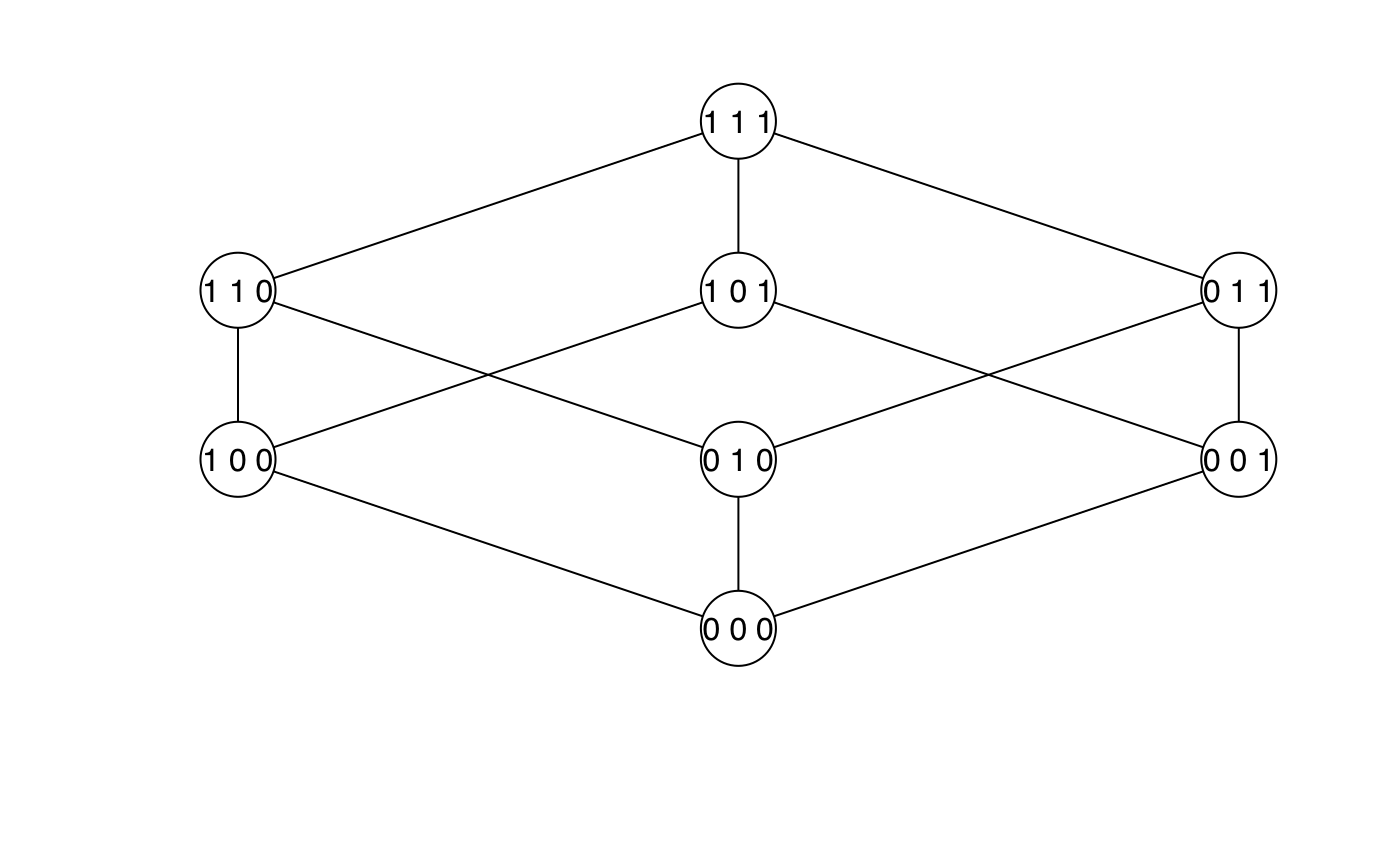
\includegraphics[width=12cm]{IMAGES/poset_4.png}
    \caption{Diagramma di Hasse.}
    \label{fig:roc}
\end{figure}

Si dice quindi che $(1,1,1)$ domina $(1,0,0)$ e si scrive $(1,0,0)\unlhd(1,1,1)$, invece $(1,1,0)$ e $(0,0,1)$ sono incomparabili e si scrive $(1,1,0)\parallel(0,0,1)$.
\\~\\
Risulta quindi chiarito che quando si ha a che fare con profili ordinali multidimensionali non si può avere un ordinamento completo, ma si adopera quello che vine chiamato \textit{ordinamento parziale}. Essendo questo tipo di dato naturalmente esprimibile secondo questo tipo di ordinamento è quindi da qui che verrà estratta l'informazione per poter generare i punteggi e quindi un ranking. Va precisato che la \textit{teoria degli ordinamenti parziali} è più generale e non è per forza legata alle variabili ordinali.


Viene ora definita in modo formale la \textit{relazione di ordine parziale} e di \textit{insieme parzialmente ordinato}.

\begin{definition}[Relazione di ordine parziale]
Sia $A$ un insieme, una \textit{relazione di ordine parziale} $\unlhd$ su $A$ è una relazione binaria (cioè un sottoinsieme del prodotto cartesiano $A\timesA$, che soddisfi le seguenti proprietà ($\forall x, y, z \in A$):
\begin{itemize}
  \item $x\unlhd x$ (\textit{riflessività})
  \item $x\unlhd y\; \& \;y\unlhd x \Rightarrow x=y $ (\textit{antisimmetria})
  \item $x\unlhd y \; \& \; y \unlhd z \Rightarrow x\unlhd z$ (\textit{transitività})
\end{itemize}
La coppia $\pi = (A, \unlhd)$ è detta \textit{insieme parzialmente ordinato} (in inglese \textit{partially ordered set} o, in breve, \textit{poset}).
\end{definition}

Per riprendere il discorso introdotto precedentemente, i poset sono rappresentabili attraverso il diagramma di Hasse, il quale si legge dall'altro verso il basso e gli elementi sono comparabili se uniti da una sequenza di discendente di link (dove l'elemento che sta più in alto \texit{domina} quello più in basso $b\unlhd a$) e al contrario se i due elementi non sono collegati da sequenze di link discendenti sono \texit{incomparabili} ($b\parallel a$). Quando due elementi sono collegati in modo diretto da un link, si dice che il superiore \textit{copre} l'inferiore. In un poset sono quindi presenti tre tipi di relazione tra gli elementi che lo compongono: \textit{copertura}, \textit{dominanza} e \textit{incomparabilità}. In un poset finito, come lo sono tutti quelli che verranno trattati, le dominanze sono ottenibili come concatenazioni delle relazioni di copertura; per esprimere questo concetto in maniera precisa diciamo che la relazione di ordine parziale è la chiusura transitiva della relazione di copertura, indicata con \prec.

\begin{figure}[H]
    \centering
    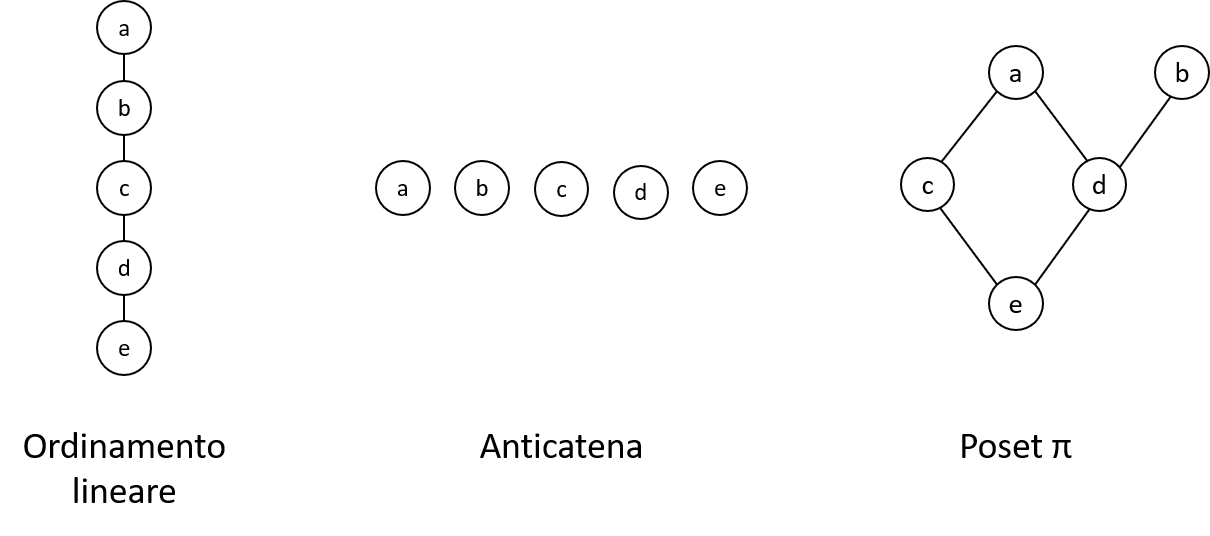
\includegraphics[width=12cm]{IMAGES/example_poset.png}
    \caption{Esempi poset.}
    \label{fig:roc}
\end{figure}

Come vediamo da figura (Figura 2.2), un poset non presenta necessariamente un \textit{massimo}, ovvero un elemento che domina tutti i restanti, e nemmeno un \textit{minimo}, ovvero un elemento dominato da tutti gli altri; tuttavia saranno sempre presenti elementi \textit{massimali}, ovvero che non sono dominati da nessun elemento, ed elementi \textit{minimali}, ovvero che non dominano nessun elemento. Sempre in figura vediamo come un poset in cui tutti gli elementi siano tra loro comparabili è chiamato \textit{lineare} (o totale, o completo, o catena), mentre un poset in cui gli elementi siano tutti incomparabili è detto \textit{anticatena}.

\section{Estensioni lineari di un poset}
Considerando i due poset presenti in figura (Figura 2.3), il $Poset\;2$ è ottenuto a partire dal $Poset\;1$ aggiungendo una comparabilità, ovvero rendendo comparabili una coppia di elementi che in partenza non lo erano. Si può quindi dire che $Poset\;1 \subset Poset\;2$.


Questa operazione di aggiunta di comparabilità è chiamata \texit{estensione} della relazione d'ordine, e consiste nel ampliare il sottoinsieme di dominanze che appartengono alla relazione, vista come sottoinsieme del cartesiano dell'insieme sul quale essa viene definita.

\begin{figure}[H]
    \centering
    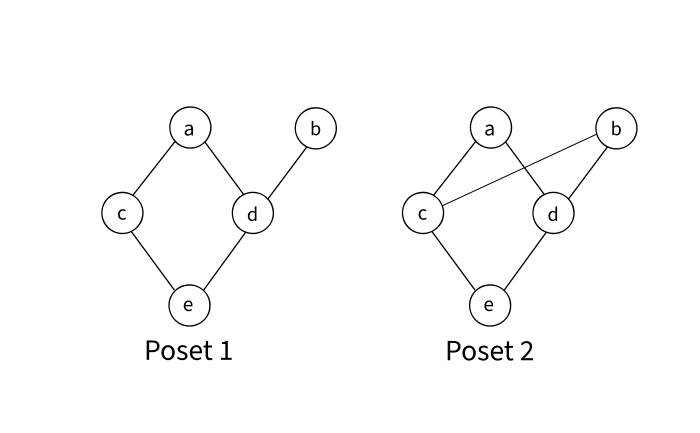
\includegraphics[width=10cm]{IMAGES/poset_5.jpg}
    \caption{Aggiunta di comparabilità.}
    \label{fig:roc}
\end{figure}


\begin{definition}[Estensione]
Dati due poset $\pi_1$ e $\pi_2$ sullo stesso insieme $X$, con i relativi ordinamenti $(X,\unlhd_1)$ e $(X,\unlhd_2)$, si dice che: 

\[ \pi_2 \;estende\; \pi_1 \Leftrightarrow \exists x,y: x\unlhd_1 y ,\; x\unlhd_2 y \land \exists p,q: p\parallel_1 q,\; p\unlhd_2 q .\]

Ovvero si dice che $\pi_2$ è un estensione di $\pi_1$ se e solo se $\pi_2$ contiene tutte le \texit{dominanze} di $\pi_1$ e c'è almeno una coppia di elementi comparabile in $\pi_2$ che in $\pi_1$ era incomparabile. 
\end{definition}

Si vede ora come perpetrando l'operazione di estensione, ovvero continuando ad aggiungere progressivamente dominanze ad un poset, si arrivi a non avere più alcuna incomparabilità, ottenendo un così detto \texit{ordinamento lineare}, come esplicitato in figura (Figura 2.4), il quale viene chiamato \texit{estensione lineare} del poset di input.

\begin{figure}[H]
    \centering
    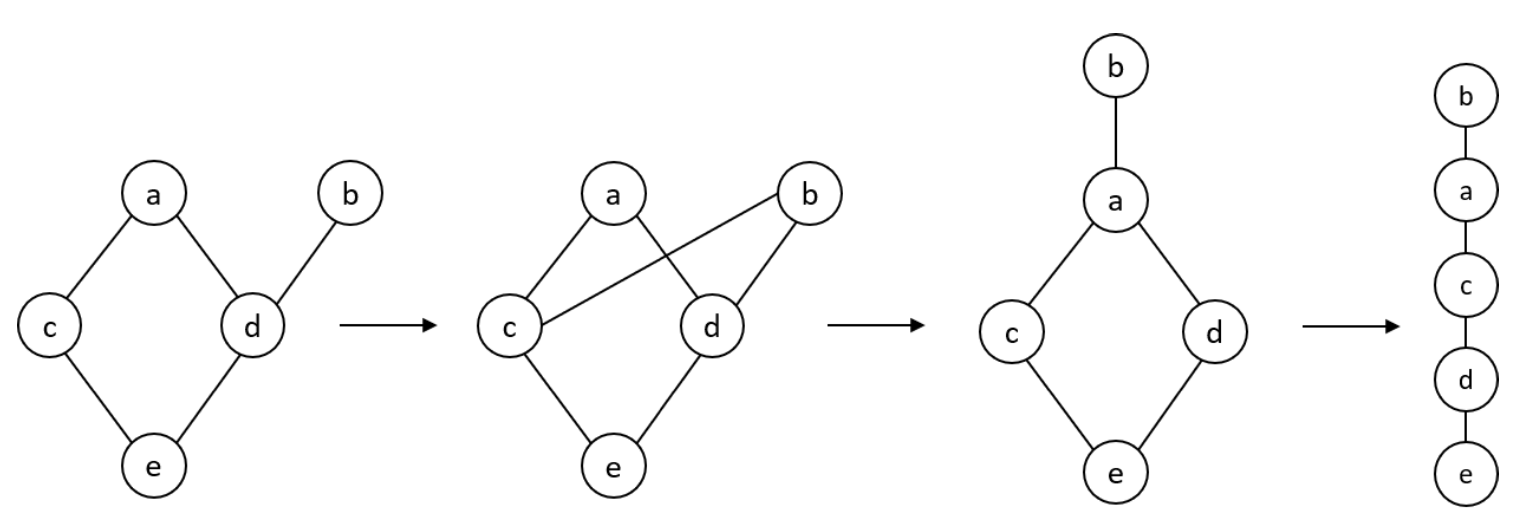
\includegraphics[width=10cm]{IMAGES/poset_6.png}
    \caption{Estensioni di un poset fino ad arrivare all'estensione lineare.}
    \label{fig:roc}
\end{figure}

Di fatto un'estensione lineare altro non è che una classifica degli elementi dal poset, che viene ottenuta compatibilmente con la struttura d'ordine, disambiguando le incomparabilità e mantenendo le dominanze. Risulta intuibile come le incomparabilità possano venire disambiguate in più modi, di conseguenza un poset non lineare é estendibile in modo lineare secondo diversi ordinamenti. Preso un poset $\pi$, la sua $i$-esima estensione lineare è indicata come $\ell_i$ e l'insieme delle estensioni lineari viene indicato come $\Omega(\pi)$.


Viene ora definita rapidamente cosa si intende per intersezione di due o più ordinamenti parziali, dato che sarà necessaria in seguito. 
\begin{definition}[Intersezione]
Per intersezione di due o più ordinamenti parziali sullo stesso insieme $A$ si intende la classica intersezione di sottoinsiemi di $A\times A$ i quali definiscono la relazione d'ordine. 
\[\unlhd_1 \bigcap_{\pi_1 \cap \pi_2} \unlhd_2 = \unlhd_n \;\vert\; \exists x,y\in \pi_1 \land \exists x,y\in \pi_2 : x \unlhd_n y \Leftrightarrow x \unlhd_1 y \land x \unlhd_2 y.\]
L’intersezione di due ordinamenti parziali sullo stesso insieme $A$ è un ordinamento parziale le cui dominanze sono tutte e sole quelle comuni agli ordinamenti parziali di input.
\end{definition}


Viene ora riportato il teorema sul quale risultato si baserà la procedura di calcolo dei punteggi e di conseguente estrazione di un ranking classica.\\

\begin{theorem}
Ogni poset finito $\pi$ coincide con l'intersezione di tutte le sue estensioni lineari.
\[\Omega(\pi)=\{\ell : \pi \subset \ell\}\Rightarrow \pi=\bigcap_{\ell \in \Omega(\pi)}\ell.\]
\end{theorem}

\renewcommand\qedsymbol{c.v.d.}
\begin{proof}
Siano $\ell_1, ..., \ell_m$ le estensioni lineari del poset $\pi$, se $x \unlhd_{\pi} y$ in $\pi$, allora $x \unlhd_{\ell_i} y$ in ogni estensione lineare $\ell_i$ e quindi $\ell_1 \cap ... \cap \ell_m$ è un'estensione di $\pi$. 
Invece ragionando per assurdo, se $x \unlhd_{\ell_i} y$, in ogni estensione lineare $\ell_i$, ovvero se la dominanza appartenesse a $\ell_1 \cap ... \cap \ell_m$, dovrebbe per forza essere $x \unlhd_{\pi} y$ in $\pi$, dato che se fosse $x \parallel y$ in $\pi$ esisterebbero due estensioni lineari $\ell_h$ e $\ell_k$ tali che $x \unlhd_{\ell_h} y$ e $x \unlhd_{\ell_k} y$, il che porta alla conclusione assurda che $y$ non dominerebbe $x$ in $\ell_1 \cap ... \cap \ell_m$. In conclusione il poset $\pi$ e l'intersezione delle sue estensioni lineari $\ell_1 \cap ... \cap \ell_m$ contengono le stesse dominanze e quindi coincidono.
\end{proof}


Non è quindi possibile che due poset $\pi_1$ e $\pi_2$, che siano diversi, abbiano esattamente lo stesso insieme $\Omega(\pi)$ di estensioni lineari.
\[\pi_1\neq\pi_2 \Leftrightarrow \Omega(\pi_1)\neq\Omega(\pi_2).\]
Questo risultato porta all'importante conclusione che lavorare sulle strutture "semplici" (ordinamenti lineari) coincide con il lavorare sul poset di input. La dimensione di un poset è quindi data dal numero minimo di estensioni lineari che sono necessarie per riottenere la struttura di input.


\section{Rappresentazioni matriciali di un poset finito}
L'obbiettivo ultimo della strutturazione delle variabili ordinali secondo i poset è quello, da un lato di preservare le informazioni derivanti da questo tipo di variabili e dall'altro di costruire degli indicatori sintetici, ovvero di costruire un ranking. Nonostante la relazione d'ordine sia un sottoinsieme del cartesiano dell'insieme sulla quale viene definita, e per questo rappresentata naturalmente dalla lista di coppie $(x, y)$ che appartengono alla relazione, ovvero per le quali vale $x \unlhd y$; per la costruzione di un ranking questa struttura risulta troppo complessa e poco manipolabile. 


Per poter ottenere gli indicatori sintetici si impongono delle rappresentazioni più semplici derivanti dal poset stesso, che lo descrivano algebricamente e che quindi permettano un estrazione facilitata dell'informazione ricercata. Le rappresentazioni in questione sono matrici che descrivono aspetti differenti della relazione di ordine parziale. 


Canonicamente le matrici usate per la descrizione di un poset sono tre, ma in questo resoconto ne verrà proposte anche altre tre, al fine di provare a superare i limiti che attualmente il sistema classico presenta. Le tre matrici "classiche" sono la \texit{matrice di incidenza}, la \texit{matrice di copertura} e la \texit{mutual ranking probability} (detta più semplicemente \texit{MRP}). Di fatto le prime due sono solamente una descrizione più compatta della relazione d'ordine, e sono tra di loro interscambiabili attraverso una formula di conversione, per quanto riguarda invece la MRP, quest'ultima rappresenta il punto chiave per l'estrazione canonica dei ranking.


Si vedono ora le proprietà fondamentali delle matrici appena introdotte. Gli esempi fatti faranno riferimento al poset raffigurato di seguito (Figura 2.5).

\begin{figure}[H]
    \centering
    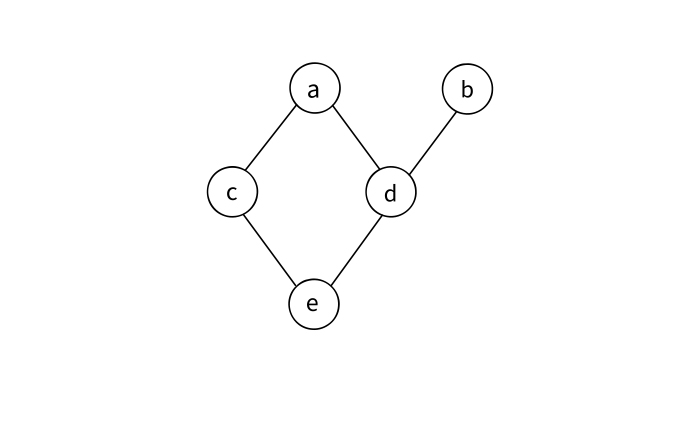
\includegraphics[width=8cm]{IMAGES/poset_7.jpg}
    \caption{Poset di esempio.}
    \label{fig:roc}
\end{figure}

\paragraph{Matrice di copertura.}
Come si è visto in precedenza, un poset è unicamente determinato dalla relazione di copertura $\prec$. Questa relazione è quella che crea la struttura per la rappresentazione grafica tramite diagrammi di Hasse. La relazione di copertura viene rappresentata tramite una matrice binaria C.
Indicando con $x_1, ..., x_n$ gli elementi dell'insieme $A$ sul quale viene definita la relazione d’ordine parziale $\unlhd$, la \texit{matrice di copertura} $C$ è una matrice $n\times n$ definita come segue:
\[C_{ij}=1\Leftrightarrow x_i \prec x_j,\]
\[C_{ij}=0 \;altrimenti.\]
Vediamo ora la rappresentazione matriciale $C$ del poset in Figura 2.5.

$C=$
\begin{blockarray}{ccccccccc}
& a & b & c & d & e  \\
\begin{block}{c(ccccccccc)}
  a & 0 & 0 & 0 & 0 & 0 \\
  b & 0 & 0 & 0 & 0 & 0 \\
  c & 1 & 0 & 0 & 0 & 0 \\
  d & 1 & 1 & 0 & 0 & 0 \\
  e & 0 & 0 & 1 & 1 & 0 \\
\end{block}
\end{blockarray}

La lettura per colonna di questa matrice $C$ indica quante volte un elemento copre gli altri, ad esempio nella matrice sopra riportata, l'elemento $c$ copre unicamente l'elemento $e$ . Invece la lettura per riga indica quanto un elemento é coperto e, sempre facendo riferimento alla matrice di sopra, l'elemento $c$ è coperto unicamente dall'elemento $a$.

\paragraph{Matrice di incidenza.}
In modo simile alla matrice di copertura, indicando con $x_1, ..., x_n$ gli elementi dell'insieme $A$ si definisce una matrice binaria $n\times n$, chiamata $Z$, che in pratica non è altro che la forma matriciale dell'elenco di coppie appartenenti alla relazione di ordine parziale $\unlhd$. Viene quindi definita come segue:
\[Z_{ij}=1\Leftrightarrow x_i \unlhd x_j,\]
\[Z_{ij}=0 \;altrimenti.\]
Come per la matrice di copertura vediamo ora la matrice $Z$ del poset in Figura 2.5.

$Z=$
\begin{blockarray}{ccccccccc}
& a & b & c & d & e  \\
\begin{block}{c(ccccccccc)}
  a & 1 & 0 & 0 & 0 & 0 \\
  b & 0 & 1 & 0 & 0 & 0 \\
  c & 1 & 0 & 1 & 0 & 0 \\
  d & 1 & 1 & 0 & 1 & 0 \\
  e & 1 & 1 & 1 & 1 & 1 \\
\end{block}
\end{blockarray}

In modo analogo alla matrice $C$ la lettura di $Z$ ha un duplice verso e senso. La lettura per colonna indica quali elementi un elemento domina, come ad esempio l'elemento $c$ domina solo se stesso ed $e$. Invece la lettura per riga indica quali elementi dominano un elemento, ad esempio l'elemento $c$ é dominato da se stesso e dall'elemento $a$. Come può risultare visibile, la relazione di copertura per la matrice $Z$ è riflessiva, ovvero un elemento copre sempre almeno se stesso, di conseguenza la diagonale della matrice di copertura sarà sempre composta da tutti 1.
\\~\\
Si riporta ora la relazione che sussiste tra le matrici $C$ e $Z$. Come anticipato in precedenza le due matrici in questione ottenibili una dall'altra, dato che la relazione di copertura di per sé determina l'ordinamento parziale e quindi la matrice di copertura implicitamente caratterizza la relazione d’ordine. Vengono ora mostrate le semplici operazioni algebriche che legano le due matrici. È necessario precisare che con $Bin(\cdot)$ si intende l'operatore che rende binarie le entrate della matrice a cui è applicato (ovvero pone uguali a 1 tutti gli elementi non nulli della matrice). 
Si riportano sotto le operazioni che legano la matrice di copertura e la matrice di incidenza:

\begin{itemize}
    \item $Z=Bin(I+C+C^2+...+C^{n-1})$, in alternativa $Z=Bin(I+C^{n-1})$.
    \item $C=Z-I-Bin((Z-I)^2)$.
\end{itemize}

Le matrici appena viste contengono tutta l’informazione necessaria a descrivere la relazione di ordine parziale, ma risultano troppo semplici quando l'intenzione è quella di costruire un ranking. La troppa semplicità di queste rappresentazioni si ha nel trattare elementi incomparabili, da qui nasce la necessità di un sistema più complesso e articolato rispetto a contare semplicemente le dominanze di un elemento.
Verrà quindi mostrata la matrice che riesce ad associate a un elemento del poset uno score che dica quanto quell'elemento è dominante. La matrice in questione non parte come quella di copertura o quella di incidenza dalla struttura base del poset ma, parte degli ordinamenti lineari che ne derivino, questo caratterizzerà la sua forza espressiva, ma anche la sua debolezza a livello computazionale.

\paragraph{Matrice Mutual Ranking Probability.}
Come detto in precedenza il motivo per cui nasce la matrice \texit{mutual ranking probability}, chiamata più semplicemente \texit{MRP}, è quello di costruire un ranking che sia in grado di porre a confronto anche quegli elementi incomparabili. Per fare un esempio dell'idea di partenza della MRP vediamo il poset sotto riportato (Figure 2.6) dove gli elementi $b$ ed $e$ sono incomparabili. Nonostante l'incomparabilità risulta possibile intuire empiricamente come in un eventuale ranking l'elemento $b$ dovrebbe trovarsi in una posizione più elevata rispetto a $e$, dato che è vicino al massimo del poset e al contrario $e$ è vicino al minimo. Intuitivamente il pensiero è che $b$ abbia qualche sorta i dominanza su $e$ che trascenda la loro incomparabilità. 

\begin{figure}[H]
    \centering
    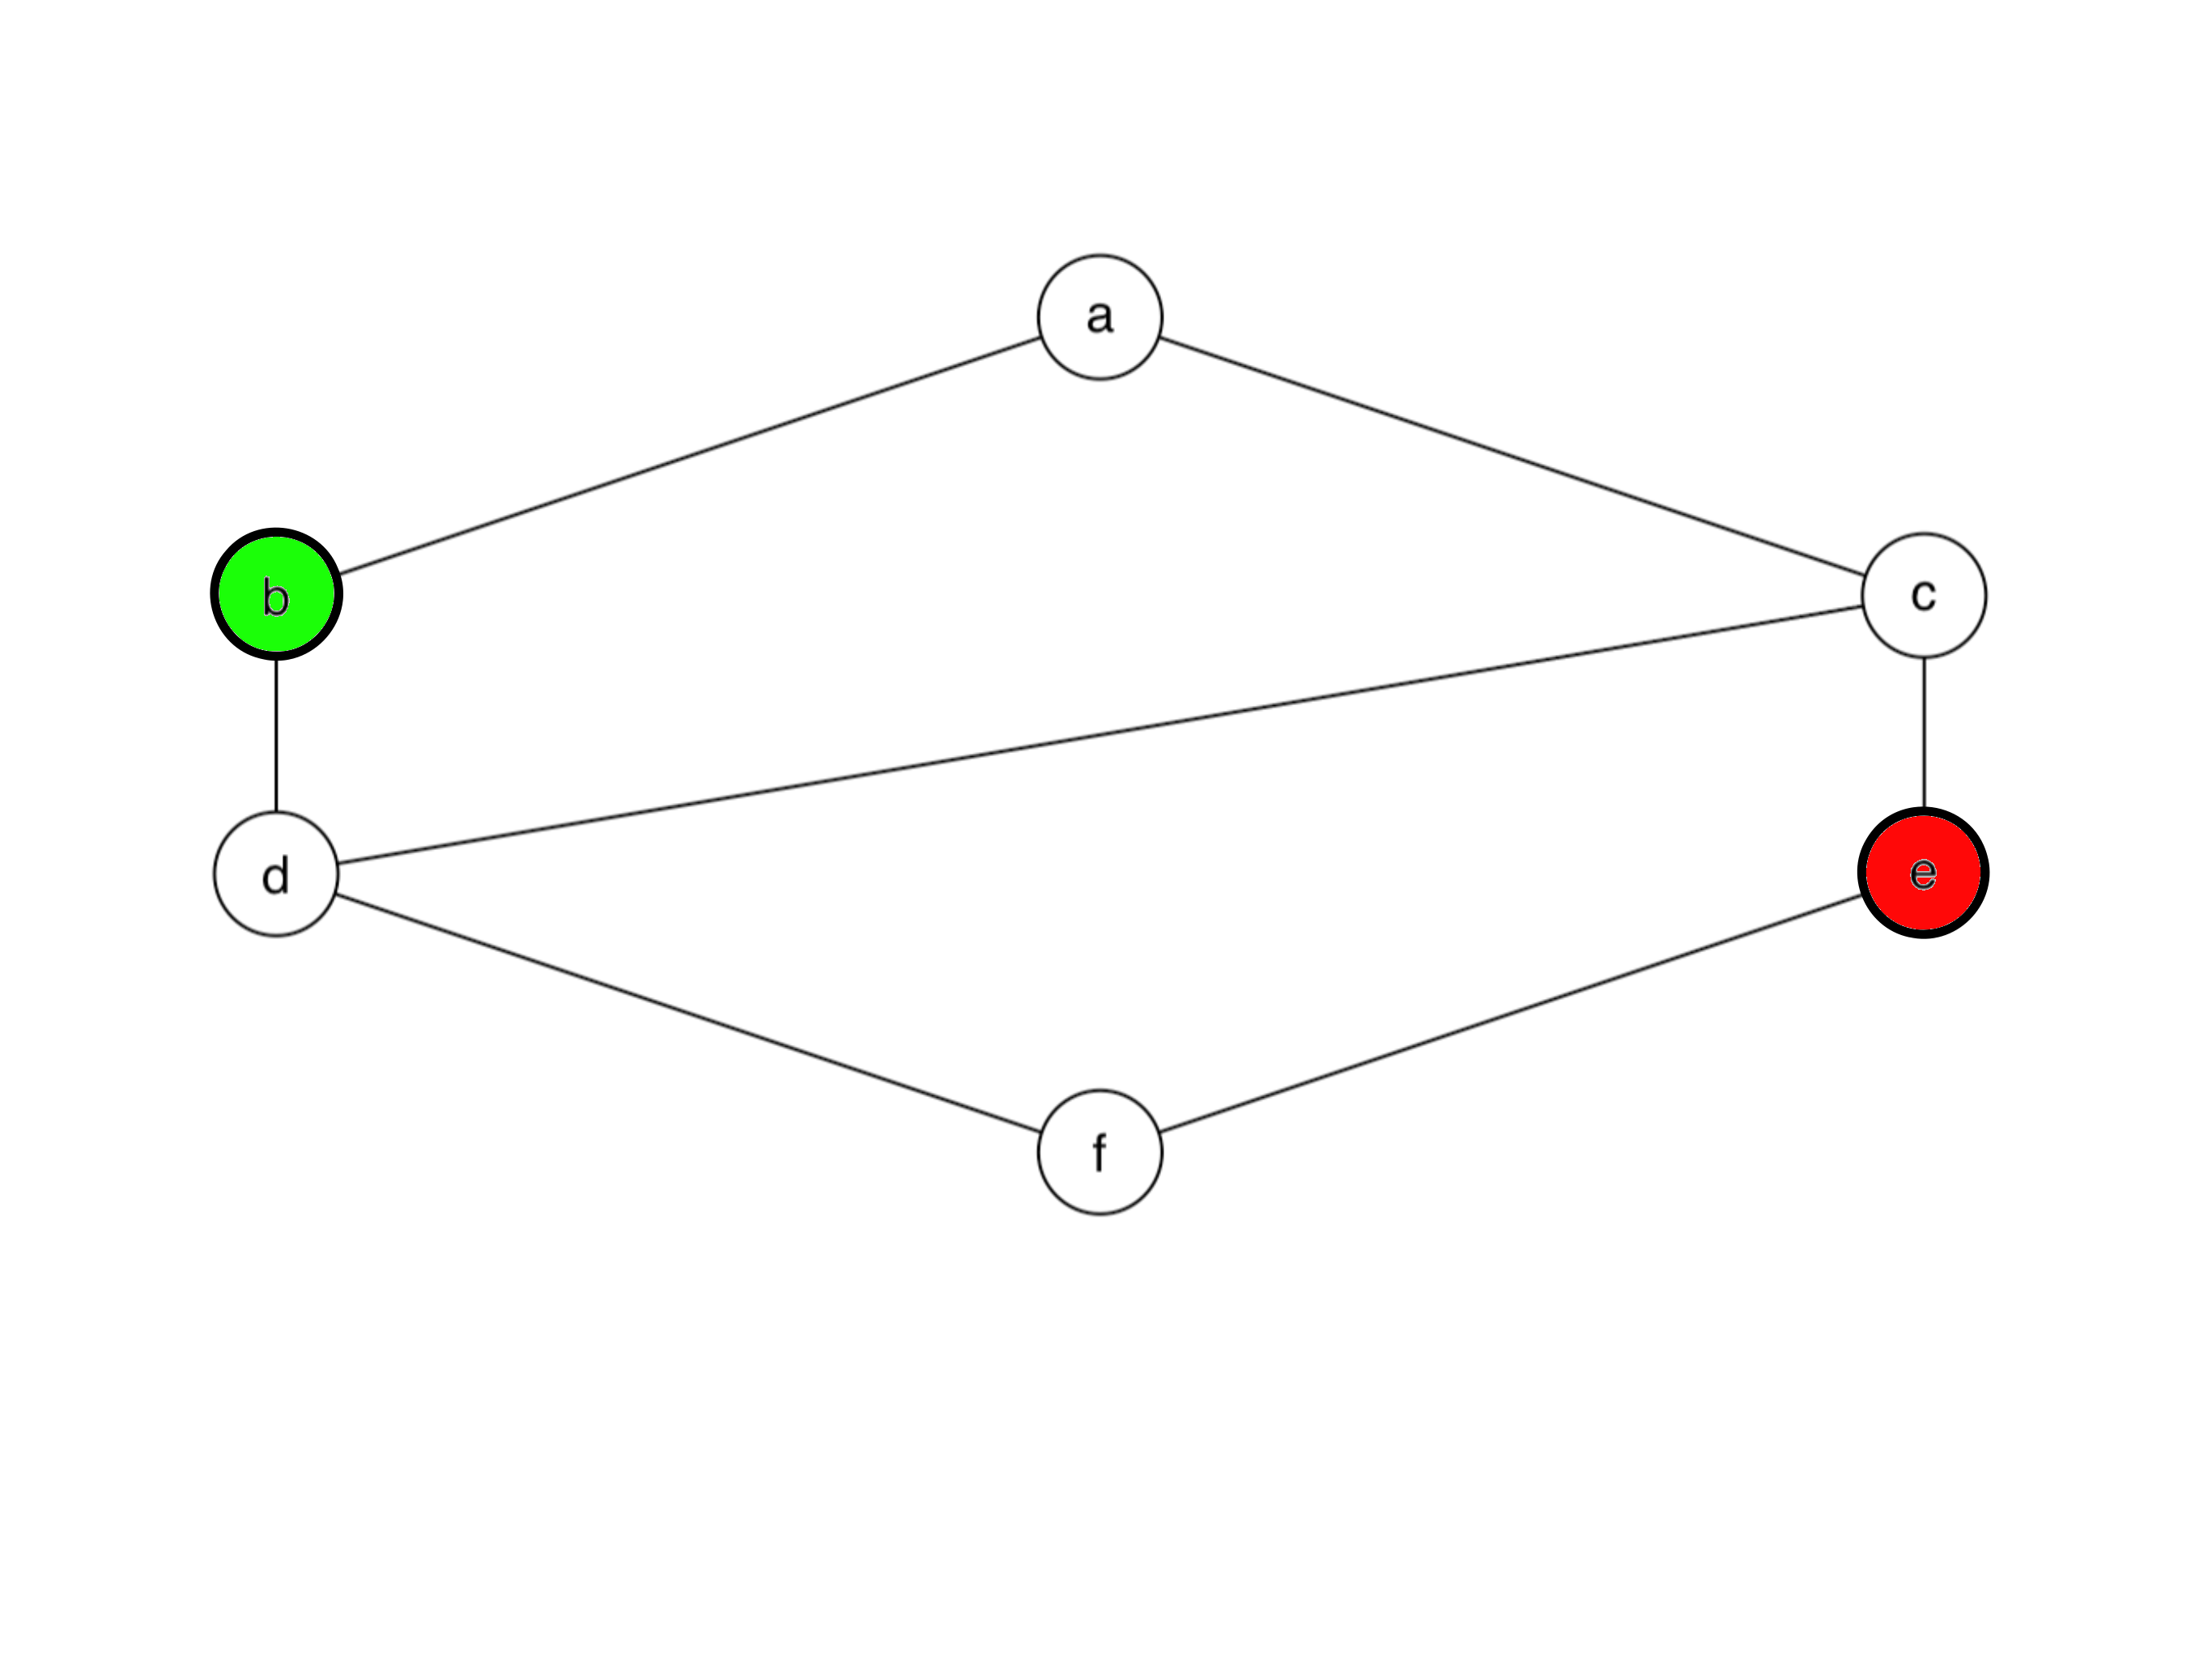
\includegraphics[width=10cm]{IMAGES/poset_8.5.png}
    \caption{Problema di incomparabilità per i ranking.}
    \label{fig:roc}
\end{figure}

Di fatto la forza della MRP è proprio quella di rendere oggettiva questa congettura. Nella matrice MRP il fatto che un elemento $x_j$ domini un elemento $x_i$ è dato dal fatto che nell'insieme di tutte le possibili estensioni lineari del poset, $x_j$ domina più volte l'elemento $x_i$, rispetto a quante volte accade il contrario.


Prima di procedere con definizione della matrice viene mostrato (Figura 2.7) il ragionamento appena fatto per l'esempio precedente. Si vede come nell'insieme delle estensioni lineari l'elemento $b$ effettivamente domini l'elemento $e$ più frequentemente di quanto accada per il contrario.
\begin{figure}[H]
    \centering
    \includegraphics[width=10cm]{IMAGES/poset_10.png}
    \caption{Estensioni lineari del poset in Figura 2.6.}
    \label{fig:roc}
\end{figure}

Il ragionamento perpetrato fino a questo momento trova una sua concretizzazione nella MRP, che è definita come di seguito:

\[M_{ij}=\frac{|\{\lambda \in \Omega(\pi): x_i \lhd_{\lambda} x_j\}|}{|\Omega(\pi)|}.\]
\\~\\
Questa definizione afferma che l'entrata $ij$-esima della matrice $M$ (MRP) è datata dal rapporto delle estensioni lineari in cui l'elemento $x_j$ domina l'elemento $x_i$ sull'insieme delle estensioni lineari del poset $\pi$.
Come succedeva per la matrice di incidenza e quella di copertura anche la MRP e la matrice di incidenza sono derivabili una dall'altra, in questo senso la matrice M è considerabile una rappresentazione matriciale del poset di input a tutti gli effetti.


Come per le matrici precedenti anche la matrice $M$ è in qualche modo derivabile dalle altre, o per meglio dire dalla matrice $Z$. Il legame che sussiste tra $Z$ ed $M$ è che dalla matrice di incidenza sono ricavabili le estensioni lineari del poset $\pi$ e quini è calcolabile la MRP con la formula appena vista. Risulta interessante notare come $M_{ij}$ sia uguale ad 1 solo se $x_i \lhd x_j$ ovvero se c'è una relazione di dominanza, quindi dove $Z_{ij}$ è uguale ad 1. Da questa relazione vediamo come sia immediato ottenere $Z$ da $M$, semplicemente ponendo a zero tutti gli elementi diversi da 1. Nel caso di un ordinamento lineare, la matrice $M$ coincide con la matrice $Z$, perché l'insieme delle estensioni lineari si riduce all'ordinamento lineare stesso, invece nel caso di un anticatena le estensioni lineari corrispondono a tutte le possibili permutazioni di tutti gli elementi e, per simmetria, ciascun elemento domina gli altri, ed è dominato dagli altri, con la stessa frequenza; per questo motivo, a parte la diagonale, tutti gli elementi sono pari a 0.5.


Si riporta ora la matrice MRP relativa al poset in Figura 2.5.

$M=$
\begin{blockarray}{ccccccccc}
& a & b & c & d & e  \\
\begin{block}{c(ccccccccc)}
  a & 1 & 2/5 & 0 & 0 & 0 \\
  b & 2/5 & 1 & 1/5 & 0 & 0 \\
  c & 1 & 4/5 & 1 & 2/5 & 0 \\
  d & 1 & 1 & 3/5 & 1 & 0 \\
  e & 1 & 1 & 1 & 1 & 1 \\
\end{block}
\end{blockarray}

Come è possibile osservare la matrice MRP è, tra le tre, quella che contiene più informazione e per questo è quella usata canonicamente per ottenere gli score e creare il ranking. Una procedura di score banalmente ottenibile consisterebbe nel sommare per colonna le entrate della matrice e cosi facendo si otterrebbero dei punteggi per costruire un ranking. Tuttavia la procedura tipicamente utilizzata è un pochino più complessa di così e il risultato punta ad avere degli score solidi e delle informazioni aggiuntive sull'incomparabilità.

\chapter{Estrazione dei punteggi e costruzione di ranking per i poset}
In questo paragrafo si affronterà il modo canonico che si adopera per ottenere un ranking da un sistema parzialmente ordinato. Come detto inizialmente, la struttura a ranking risulta particolarmente efficace se applicata a variabili ordinali, dato che in modo teorico gradi alti delle variabili corrispondono a punteggi maggiori, di conseguenza a valutazioni migliori e quindi a posizioni più elevate nel ranking. La procedura di estrazione del ranking da un poset consiste nell'estrarre quelle informazioni necessarie per associare un punteggio di dominanza degli elementi che lo compongono cosi da costruire il ranking basandosi su questi punteggi. Ovvero quello che si vuole ottenere è che elementi più vicini al massimo abbiano posizioni più elevate nel ranking.


Come introdotto in precedenza la matrice MRP riesce ad esprimere questa informazione e di conseguenza sarà la matrice di partenza per l'estrazione degli score e per la creazione di un ranking.
Quello che si vuole ottenere è una funzione $s(\cdot)$ detta \textit{funzione di scoring} che sia in grado di \textit{preservare strettamente l'ordine}.

\[s(\cdot): \pi \mapsto R^{+} \cup 0 \;|\; \forall x_i,x_j : x_i \lhd x_j \Rightarrow s(x_i) < s(x_j).\]

Ovvero si vuole ottenere una funzione tale per cui, dato il poset $\pi$, la funzione $s(\cdot)$ assegni punteggio maggiore all'elemento $x_j$, rispetto che all'elemento $x_i$, se valesse che $x_j$ domina $x_i$. La funzione di scoring da cui seguirà il ranking viene costruita a partire dalla matrice MRP.


Si vede ora come utilizzando la \textit{decomposizione a valori singolari} sia possibile utilizzare l'autovettore relativo all'autovalore maggiore della matrice come funzione per ottenere uno score robusto.  Naturalmente è possibile usare altri tipi di score e generare altri indicatori alternativi di dominanza, come ad esempio può esserci una funzione di scoring che lavora semplicemente sommando le colonne di M ma, queste altre funzioni, risultano meno efficaci. La funzione di scoring che verrà mostrata è detta \texit{average rank} di $x_i$ e corrisponde alla media delle posizioni di $x_i$ nell'insieme $\Omega(\pi)$ delle estensioni lineari del poset $\pi$.

\begin{definition}[Average rank]
Dato un poset finito $\pi$ composto da $n$ elementi, prendendo la matrice $M$, ovvero la matrice MRP relativa, se ne applica la decomposizione a valori singolari (decomposizione SVD) e, cosi facendo, si ottiene $M=UDV^T$.
Prendendo la prima colonna di $V$, $ \textbf{v} = (v_1, ...,v_n)$, ovvero l'autovettore della matrice MRP relativo all'autovalore maggiore, si definisce la funzione di scoring tale che $s(x_i) = v_i$.
\end{definition}

\renewcommand \qedsymbol{c.v.d.}
\begin{proof}
La definizione, affermando che la prima colonna di $V$, $ \textbf{v}$, sia una funzione di scoring, afferma che le componenti del primo autovettore di $M^TM$ associate agli elementi $x_1, ...,x_n$ preservano strettamente l'ordine e sono non negative.
Il \texit{Teorema di Perron-Frobenius} garantisce la non negatività delle componenti dato che la matrice di input è non negativa. Si procede ora a provare che l'ordine sia preservato strettamente, ovvero che  $x_i \lhd x_j \Rightarrow s(x_i) < s(x_j)$. 
Si vede come la prima colonna di $V$ sia una combinazione lineare delle colonne di $M^T$, con coefficienti dati dalla prima colonna di $U^T$ moltiplicata per il primo elemento della diagonale di $D^{-1}$. Questo si ottiene avendo applicato la scomposizione SVD alla matrice $M$ e da cui si ottiene la relativa scomposizione $M=UDV^T$, ed esplicitando $V$ si ha che $V=M^TUD^{-1}$.
Sempre per il \texit{Teorema di Perron-Frobenius} i coefficienti ottenuti sono non negativi, da cui segue che la prima colonna di $V$, $ \textbf{v}$, è il vettore delle somme pesate del vettore delle mutual ranking probability degli elementi $x_1, ...,x_n$. Ovvero presa $i$-esima componente $v_i$ essa altro non è che una somma pesata del vettore delle mutual ranking probability del $i$-esimo elemento $x_i$, ovvero informazione del suo livello di dominanza contenuto nella $i$-esima colonna della matrice MRP.
Fatta questa specificazione, è ora possibile mostrare come queste componenti preservino l'ordine, confrontando la colonna $i$-esima e la colonna $j$-esima di M quando vale che $x_i \lhd x_j$.
Si osserva che dato, il poset $\pi$ e $i\neq j \neq h$, se $x_i \lhd_{\pi} x_j$ e se $x_h \lhd_{\lambda} x_i$ nell'estensione lineare $\ell$, allora vale che $x_h \lhd_{\ell} x_j$. Da questo si ottiene che $x_j$ domina $x_h$ con un grado maggiore rispetto a quanto $x_i$ domini $x_h$, ovvero che $M_{hi} \leq M_{hj}$. Inoltre dato che $x_i \lhd x_j$ vale che $M_{ij}=1$ e $M_{ji}=0$ e si sa che per costruzione $M_{ii}=M_{jj}=1$. Da questi aspetti deriva che $v_i<v_j$, dato che ogni elemento della colonna $j$-esima di $M$ è maggiore o uguale al corrispondente elemento della colonna $i$-esima e almeno un elemento è maggiore in senso stretto; quindi la somma pesta degli elementi della colonna $j$-esima è strettamente maggiore della somma pesata degli elementi della colonna $i$-esima.
Cosi facendo si è dimostrato che  $s(x_i) = v_i$ è una funzione di scoring che preserva strettamente l'ordine ed è non negativa.
\end{proof}

Si è appena visto che basta considerare le componenti del primo vettore singolare destro, che di fatto non sono altro che somme pesate dei gradi di dominanza delle singole variabili, per poter generare una misura sintetica che, una volta ottenuti i punteggi, verrà poi espressa sotto forma di ranking considerando la classifica che ne deriva.
\\~\\
Quando si ha a che fare con sistemi multi dimensionali di indicatori, spesso succede che due unità statistiche abbiano lo stesso profilo e per questo motivo vengano classificate pari-merito. In questo caso, quindi, l'insieme delle unità non è più considerabile un sistema parzialmente ordinato, poiché non vale più l'\textit{antisimmetria} (una delle tre condizioni che definiscono la struttura di poset). Per quanto riguarda invece le proprietà di \textit{riflessività} e \textit{transitività}, esse continuano a valere. La struttura matematica in questione è chiamata \textit{quasi-ordine}. In questo caso per ottenere gli score, per poi costruire il ranking, si assegna ad ogni coppia di elementi la matrice MRP dei relativi profili e si costruisce una matrice in cui a unità statistiche di uguale profilo corrispondono righe e colonne di MRP identiche.
La matrice che si ottiene così facendo è singolare e si procede con la SVD come in precedenza per calcolare gli score di dominanza, attuando questo cambiamento si fa si che unità statistiche con stesso profilo abbiano lo stesso score e quindi stessa posizione nel ranking. Il procedimento è analogo anche nel caso di poset con assegnati pesi, ovvero dove ad ogni elemento è associata una frequenza.




\\~\\
Viene ora riportato un esempio della procedura di ranking su un poset.
Il poset in questione è un poset semplice con un elemento incomparabile da tutti gli altri, come visibile in figura (Figura 3.1).

\begin{figure}[H]
    \centering
    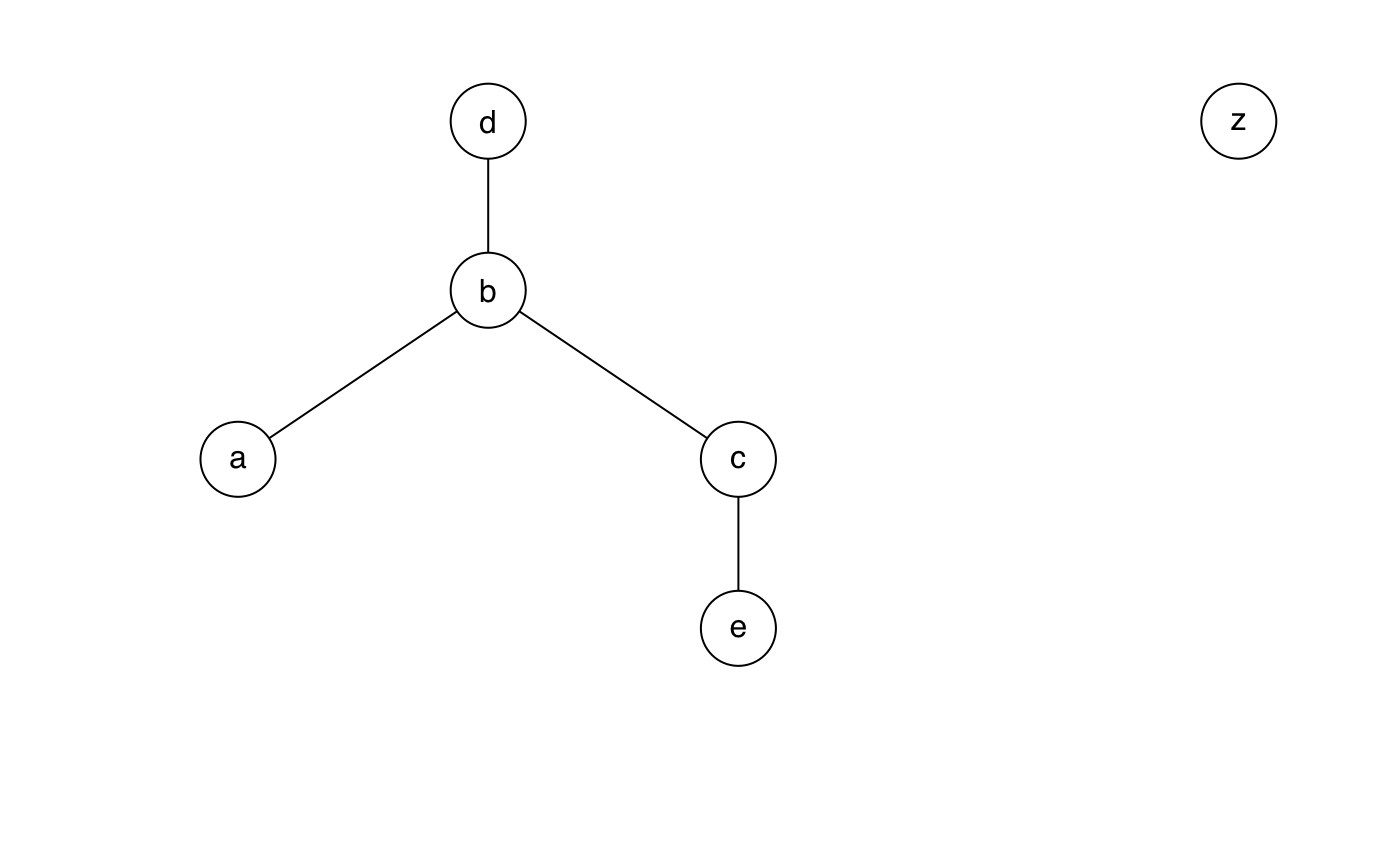
\includegraphics[width=8cm]{IMAGES/poset_11.png}
    \caption{Poset di esempio.}
    \label{fig:roc}
\end{figure}

Si procede mostrando la matrice MRP relativa al poset, ottenuta come spiegato in precedenza, ovvero valutando le estensioni lineari.

$M$ =
\begin{blockarray}{ccccccc}
& a & b & c & d & e & z \\
\begin{block}{c(ccccccccc)}
  a & 1.00 & 1.00 & 0.67 & 1.00 & 0.33 & 0.67 \\
  b & 0.00 & 1.00 & 0.00 & 1.00 & 0.00 & 0.33 \\
  c & 0.33 & 1.00 & 1.00 & 1.00 & 0.00 & 0.56 \\
  d & 0.00 & 0.00 & 0.00 & 1.00 & 0.00 & 0.17\\
  e & 0.67 & 1.00 & 1.00 & 1.00 & 1.00 & 0.78\\
  z & 0.33 & 0.67 & 0.44 & 0.83 & 0.22 & 1.00\\
\end{block}
\end{blockarray}

Dalla matrice $M$ si ottengono gli score, sempre come visto in precedenza, attraverso l'autovettore relativo all'autovalore maggiore. Dai punteggi di score ottenuti ne deriva poi, ponendo gli elementi in ordine decrescente, il ranking degli elementi del poset di input (Tabella 3.1).

\begin{table}[H]
\centering
	\begin{tabular}{l c c}
	& Elementi & Score & Ranking \\
	\hline
    \ang{1} &	d &	0.5720778 \\		
    \ang{2} &	b &	0.5155088 \\		
    \ang{3} &	z &	0.3807146 \\		
    \ang{4} &	c &	0.3753416 \\		
    \ang{9} &	a &	0.2850330 \\		
    \ang{6} &	e &	0.1997720 \\		
    \hline
    \end{tabular}
    \caption{Ranking con score. \label{t:table}}
\end{table}

Nell'esempio appena proposto si vuole osservare in particolare l'elemento $z$. Questo elemento risulta incomparabile con tutti gli altri elementi, dunque empiricamente se si dovesse pensare ad un ranking (senza fare la procedure MRP) si avrebbe difficoltà a valutare in che posizione piazzarlo. Come si nota l'elemento $z$ viene posizionato più o meno a metà classifica, questo succede perché essendo slegato di fatto dall'ordinamento ogni estensione lineare che ci sarebbe senza l'elemento $z$ vede una propria variante dove quest'ultimo ricopre, di volta in volta, tutte le posizioni dalla prima all'ultima.

\\~\\
L'esempio chiarisce come gli score di dominanza e il relativo ranking siano delle sintesi che, di fatto, forzano la complessità del poset di input in uno struttura di output semplificata (essendo appunto delle sintesi). Queste forzature risultano più o meno inficianti ma la cosa importante è il riuscire a riconoscerle e poterle valutare.
Per fare ciò esistono degli strumenti specifici che servono appunto a valutare il grado di queste forzature.


Per valutare il grado di forzatura nel ranking derivanti da un poset, viene ora introdotta la \textit{matrice di incomparabilità} $I$:
\[I_{ij}=min(M_{ij},M_{ji}).\]
Ovvero una matrice dove l'elemento $ij$ rappresenta il grado di incomparabilità fra $x_i$ e $x_j$, è quindi per definizione una matrice simmetrica che fornisce informazione su quanto i singoli elementi siano comparabili con gli altri.
Il grado di incomparabilità tra due elementi, identificato dalla matrice $I$, varia tra 0 e 0,5, ed è tanto più vicino a 0.5 quanto più simili sono i gradi di dominanza tra i due elementi vicendevolmente. Chiaramente più incomparabilità saranno presenti in un poset più lo scoring e di conseguenza i ranking saranno una forzatura. 


Per ottenere una misura sintetica che misuri l'incomparabilità di ogni elemento del poset si procede considerando le componenti del primo autovettore di $I$ che per il \textit{Teorema di Perron-Frobenius} è ad entrate non negative. 

\begin{definition}[score di incomparabilità]
Dato un poset finito $\pi$ composto da $n$ elementi, prendendo la matrice $I$ (che per il \textit{Teorema di Perron-Frobenius} è ad entrate non negative), ovvero la matrice di incomparabilità relativa, se ne applica la decomposizione a valori singolari, che essendo la matrice simmetrica corrisponde ad una decomposizione spettrale.
Prendendo quindi le componenti del primo autovettore di $I$, $ \textbf{i} = (i_1, ...,i_n)$, si definisce la funzione per valutare l'incomparabilità, di ogni elemento del poset, tale che: 
\[inc(x_j) = i_j.\]
\end{definition}

Ottenuto anche il punteggio di incomparabilità ad ogni unità statistica si assoceranno quindi due punteggi, uno di dominanza e uno di incomparabilità, i quali possono essere utilizzati per costruire visualizzazioni bidimensionali dei dati. 
Solitamente la forma che caratterizza queste rappresentazioni è simile a quella in figura (Figura 3.2) dove gli elementi che occupano le posizioni centrali del ranking sono quelli con uno score di incomparabilità, mentre più ci si avvicina ai vertici più gli elementi sono comparabili.

\begin{figure}[H]
    \centering
    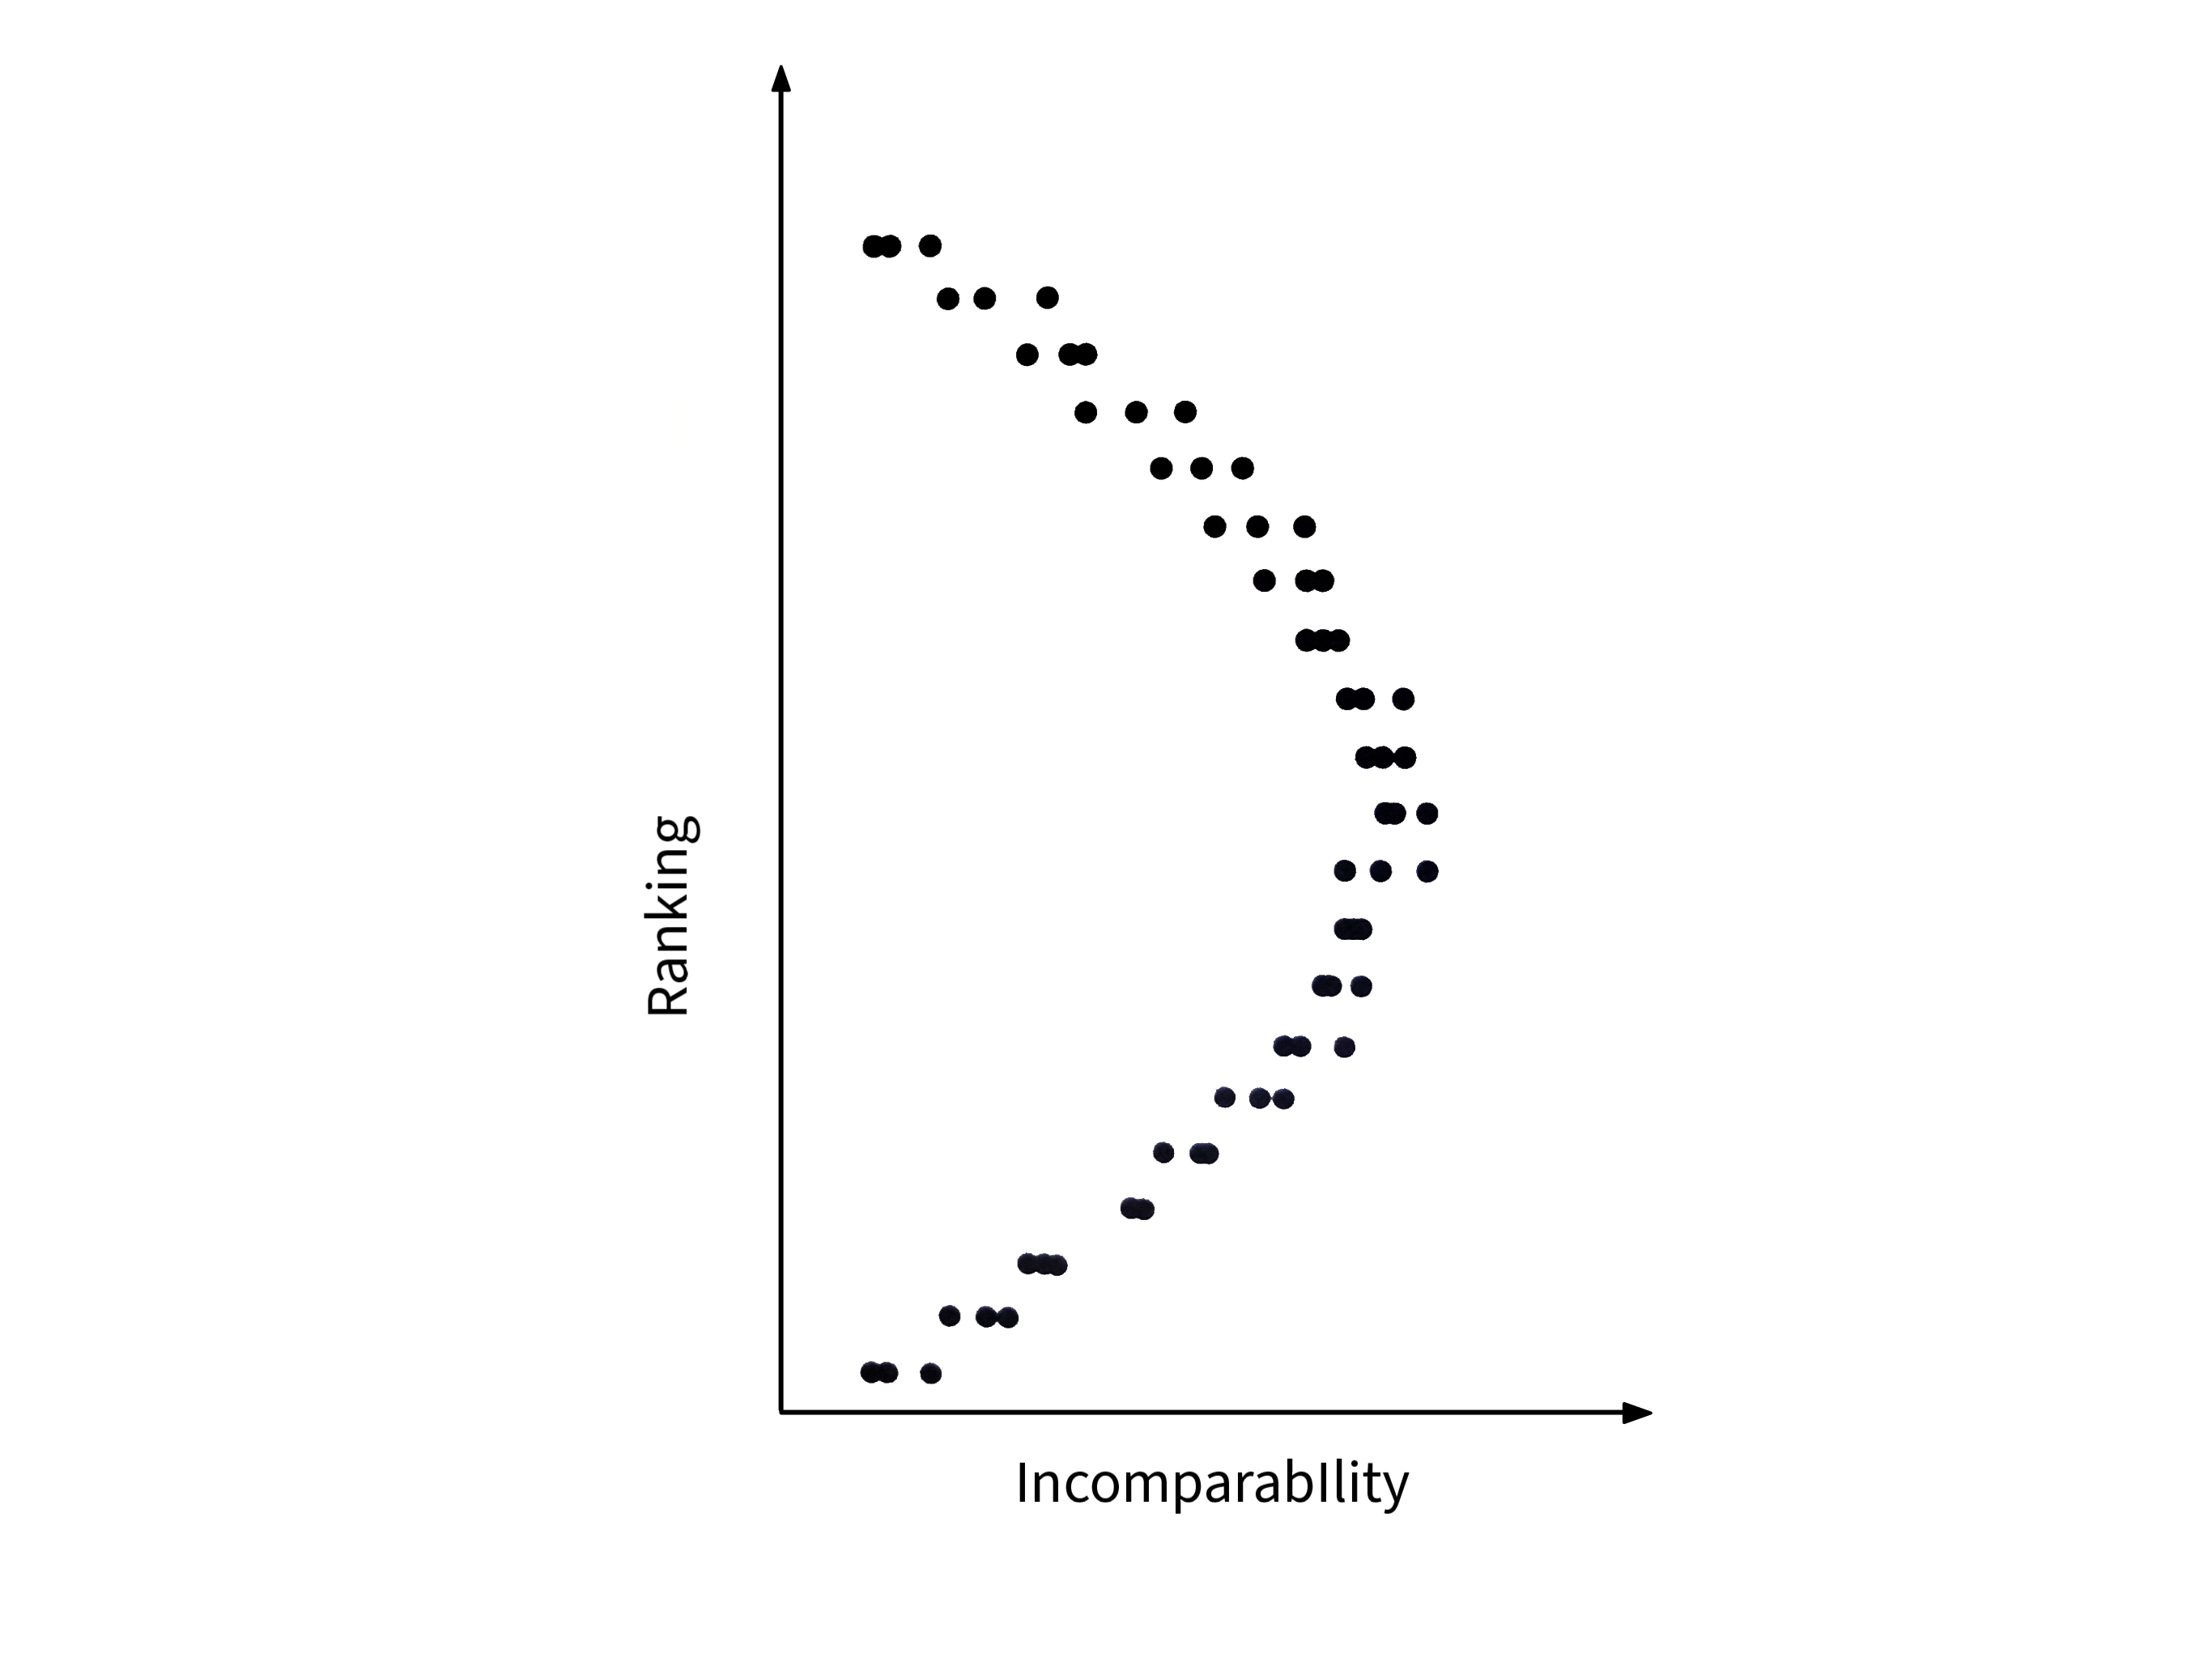
\includegraphics[width=8cm]{IMAGES/image ranking.png}
    \caption{Forma tipica del grafico di ranking e incomparabilità.}
    \label{fig:roc}
\end{figure}

Per completezza viene mostrata anche una rappresentazione analoga per poset, in Figura 3.1, preso in considerazione per gli esempi fino ad ora (Figura 3.3).

\begin{figure}[H]
    \centering
    \includegraphics[width=8cm]{IMAGES/Schermata 2022-07-01 alle 10.05.23.png}
    \caption{Ranking e incomparabilità del poset di esempio.}
    \label{fig:roc}
\end{figure}

Si vede chiaramente come l'elemento $z$ si discosti da gli altri rappresentando una forzatura, tuttavia anche elementi collegati al nodo centrale, come l'elemento $a$ possono risultare scostati. In generale il poset in questione è piccolo e diramato subito e in questo troviamo la causa di tali forzature.
\\~\\
Il sistema di ranking costruito fino a questo momento risulta una sintesi particolarmente solida ed efficace a livello visivo e concettuale. Un output di questo genere è necessario quando si ha che fare con i sistemi parzialmente ordinati per poter fare chiarezza sulle informazioni intrinseche di un poset. Come detto precedentemente avere una classifica, sopratutto quando abbiamo a che fare con variabili ordinali, risulta un punto chiave, per questo motivo queste strutture matematiche risultano così importanti e altrettanto importante risulta il generare un output chiaro e leggibile che produca una classifica degli elementi su cui poi fare le dovute analisi.

\chapter{Il problema computazionale della MRP}
Il sistema di ranking e di valutazione costruito a partire dalla matrice MRP risulta molto solido e particolarmente espressivo, tuttavia questa procedura è affetta da un grave onere computazionale, che risulta in tempi di elaborazione molto lunghi specialmente all'aumento della complessità del poset di input. Il problema computazionale si verifica per il calcolo della matrice MRP, la complessità si trova nel calcolo delle estensioni lineari del poset di input, poiché oltre a richiedere una tempistica non indifferente per l'estrazione di una singola, la quantità delle estensioni lineari per poset un minimo involuti è enorme. Anche il calcolo del numero di estensioni lineari di un poset risulta complesso. Per l'appunto il calcolare il numero di estensioni lineari di un poset è un problema P-completo \citep{brightwell1991} e per questo motivo non è possibile trovargli una soluzione ottimale nel caso generale. Per poter comprendere la complessità del problema in questione e il perché, come vedremo in seguito, sia stato necessario trovare delle approssimazioni per il calcolo, è necessario portare un esempio. L'esempio in questione viene ripreso da \citet{fattore2018}.


Si considera ora il poset riportato in Figura 1, esso fa parte della classe di poset $\{2^k\} (k=1, 2, 3, ...)$, ovvero quei poset generati da $k$ catene di due elementi. Il poset in questione in particolare è $2^3$. Ovviamente aumentando il valore di $k$ il numero di elementi del poset aumenta, per esempio $2^2$ ha 4 elementi, $2^3$ ha 8 elementi e $2^4$ ne ha 16. Come detto in precedenza non esiste una soluzione standardizzata per il calcolo del numero di estensioni lineari, per questo motivo risulta anche difficile il capire la complessità del problema. 
Non essendo quindi possibile fare riferimento al numero esatto di estensioni lineari, se non per i poset più semplici per cui è possibile calcolarle in tempi brevi, si sceglie di considerare il limite inferiore, in modo che comunque si possa avere una visione della grandezza della problematicità computazionale.
Il numero di estensioni lineari del poset $2^k$, esponente di questa famiglia di poset, viene indicato come $|\Omega(2^k)|$. Il limite inferiore per il numero di estensioni lineari di $2^{k+1}$ è dato da:
\[|\Omega(2^{k+1})|>(k+1)\cdot |\Omega(2^k)|^2 + \prod_{s=1}^{k+1}\left[ \left( \begin{array}{c} k+1 \\ s \end{array} \right)! \right].\]

Come appena detto quindi non si considera il numero preciso di estensioni lineari $|\Omega(2^k)|$ ma, piuttosto, il suo limite inferiore. Osservando il risultato riportato in tabella (Tabella 4.1) si nota come, aumentando di poco il numero di elementi, il numero di estensioni lineari diverse possibili diventi enorme.


\begin{table}[H]
\centering
	\begin{tabular}{l c c}
	& Elementi & Estensioni lineari & Poset \\
	\hline
	2^1 & 1 & 1 \\
	2^2 & 4 & 2	\\
	2^3 & 8 & 48 \\
	2^4 & 16 & $>423,936$ \\
	2^5 & 32 & $>1.8\times10^{17}$ \\
	\hline
	\end{tabular}
\caption{Numero di estensioni lineari.\label{t:table}}
\end{table}

La tabella mette alla luce l'enorme onere computazionale che la macchina deve affrontare per il calcolo della matrice MRP.


Come si è appena visto, già a partire da poset di "semplice" costruzione, come quelli della famiglia $\{2^k\}$ il numero di estensioni lineari esplode. Nella realtà, a meno di problemi particolari, capita spesso che i poset abbiano attributi non solo binari, ma con un numero di gradi più elevato, questo porta a risultati estremamente più complessi con numeri estremamente maggiori di quelli appena visti. In conclusione la matrice MRP, nonostante sia fondamentale per i ranking non è calcolabile in tempi utili, per questo motivo, come viene riportato nel prossimo capitolo, è necessario ricorrere ad approssimazioni o a soluzioni alternative.

\chapter{Soluzioni standard per il problema computazionale della MRP}
Per la tecnologia ad oggi esistente e per la capacità di calcolo di cui le macchine moderne sono capaci il calcolo della matrice MRP, su poset non "banali", risulta troppo complesso a causa della necessita di generare un numero immenso di estensioni lineari. È quindi chiaro come sia necessaria una soluzione per avere dei risultati attendibili in tempi utili. 


Vengono ora presi in rassegna i due apporci principali, in modo da presentare le metodologie secondo le quali odiernamente si procede per questo calcolo. Gli apporci presentati sono, l'\textit{approccio completo}, ovvero la stima della MRP per la sua interezza attraverso algoritmi il più efficienti possibili che, come già anticipato, risulta molto oneroso e di una pesantezza computazionale estrema; e l'\textit{approccio campionario}, ovvero il metodo classici di "risoluzione" di questo problema che fa fronte ad algoritmi di campionamento in modo da poter ottenere una stima verosimile della matrice MRP, estraendo solamente un sottoinsieme di $\Omega(\pi)$. In generale quindi le soluzioni esistenti per trovare una risposta al problema puntano alla ricerca di algoritmi sempre più efficienti per la ricerca o di tutte le estensioni lineari o del campionamento migliore. Oltre a dare una visione su questi due approcci, li si confronterà e si metteranno in luce le debolezze di entrambi.


Risulta ora necessario precisare che i poset non sono strutture adoperate nella Big Data anlysis. I problemi computazionali come si è visto sono presenti anche per poset con meno di 20 elementi, questo fa si che per la Big Data anlysis la risoluzione di questo problema sia pressoché impossibile. Oltre al mero fatto computazionale, i problemi reali in cui risulta utile l'utilizzo di queste strutture matematiche sono problemi numericamente contenuti. Come citato nel primo capitolo, i poset sono spesso usati per problemi di natura socio-economica, ed in questi casi il numero di elementi molto raramente supera le 100 elementi; in generale non ci sono problemi reali (se non per studio del comportamento matematico delle strutture) in cui gli elementi si avvicinino e superino 1000 elementi. 


Come sopra precisato, vengono presi in rassegna i due metodi e, per presentarli, vengono citati due algoritmi che si adoperano nella pratica. In particolare vengono usate come esempio gli algoritmi implementati nella funzione \texttt{LEapply} nel pacchetto \texttt{R} chiamato \texttt{POSetR}. La funzione in questione è una delle più efficaci odiernamente implementate e comprende un algoritmo per la generazione completa delle estensioni lineari e un algoritmo MCMC per il campionamento quasi-uniforme delle estensioni lineari, permettendo di poter scegliere tra i due.


\section{Approccio completo.}
Come in parte è già stato introdotto in precedenza, il numero di estensioni lineari per poset non banale è enorme e quindi, nonostante l'efficacia degli algoritmi trovati per la generazione della MRP nella sua completezza, il problema persiste ancora. L'algoritmo usato vien discusso da \citet{habib2001efficient}.


I diversi algoritmi presentati sono efficienti con la migliore complessità temporale possibile, fino a fattore costante. Purtroppo però gli algoritmi funzionano a tempo costante per alcune classi speciali di poset, il trovare un algoritmo a tempo ammortizzato costante rimane ancora un problema per il caso generale. Quindi, in generale, produrre tutte le estensioni lineari di un poset rimane fattibile solo per esempi banali. Sono perciò necessarie soluzioni diverse per poter utilizzare queste strutture nella pratica. 

Prendendo in esempio i poset in figura (Figura 5.1) tra cui, i poset della famiglia $2^k$, si osservano le tempistiche di computazione su una macchina dalle medie capacità di calcolo con un processore "2.8 GHz Intel Core i7 quad-core".
\begin{figure}[H]
    \centering
    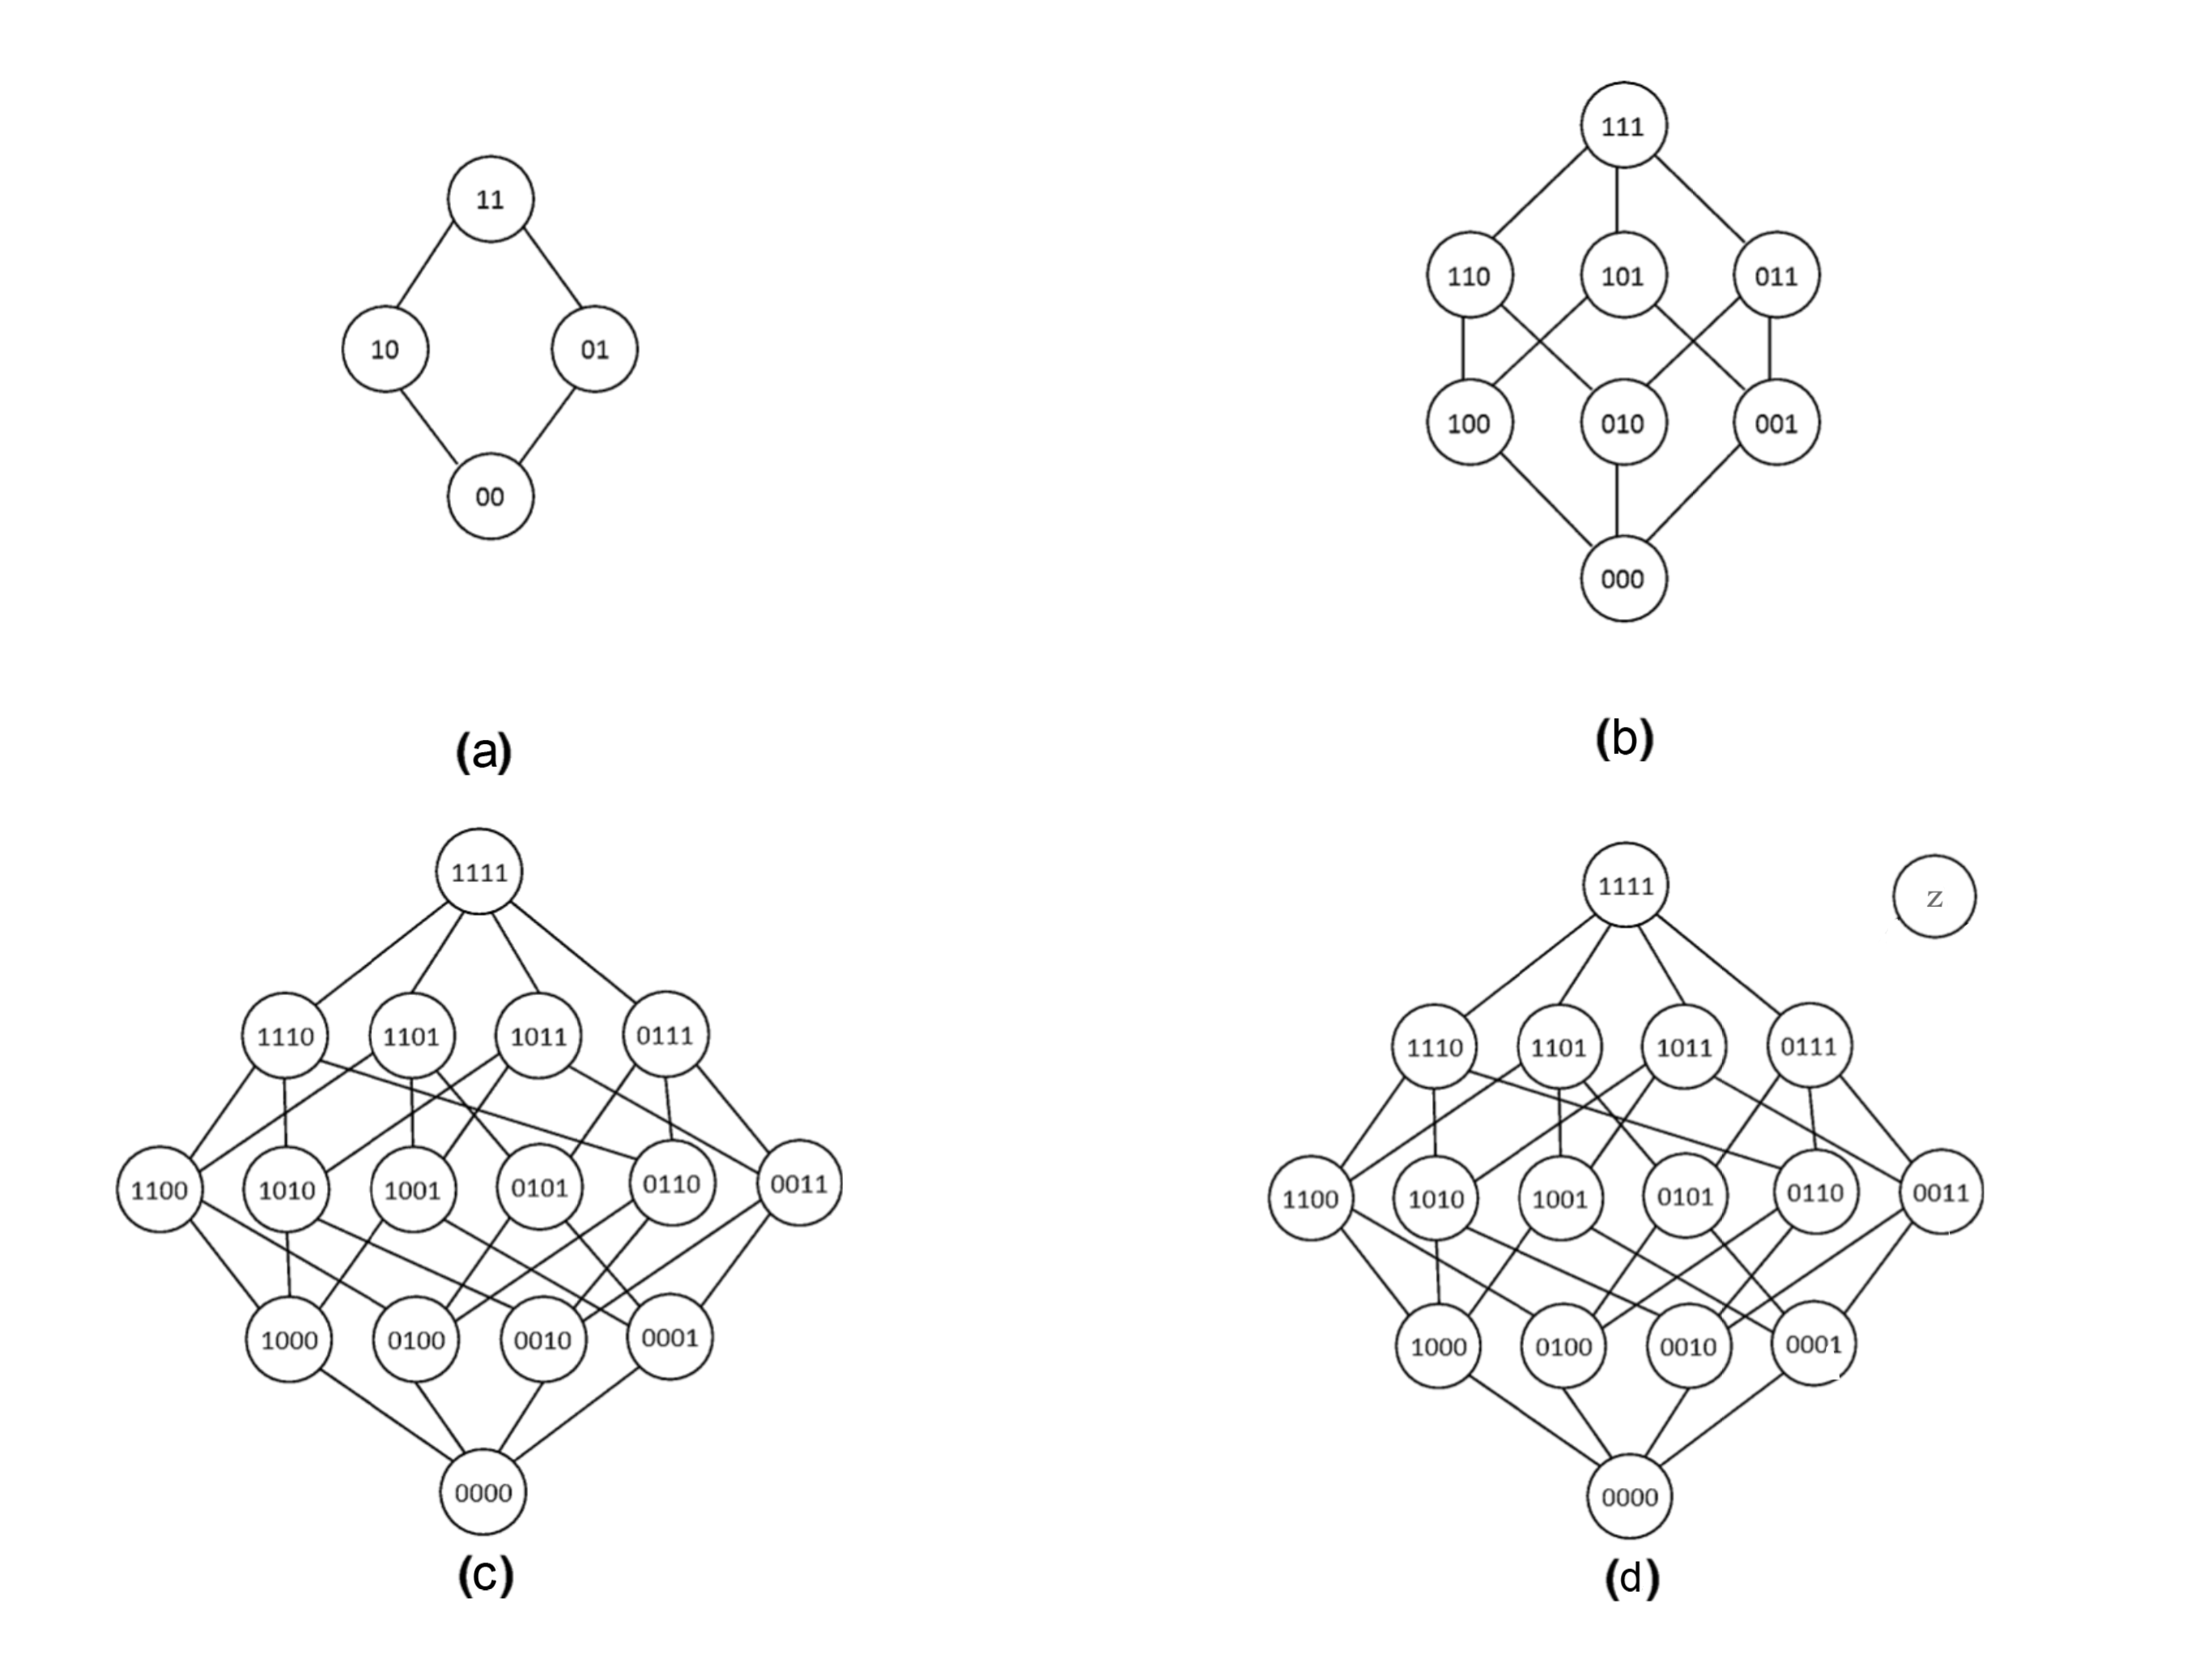
\includegraphics[width=10cm]{IMAGES/poset_12.png}
    \caption{Poset $2^2$ (a), $2^3$ (b), $2^4$ (c), $2^4$ con elemento incomparabile (d).}
    \label{fig:roc}
\end{figure}

Vengono ora riportati i tempi di computazione della matrice MRP per i poset appena citati. Ci si aspetta che il tempo di calcolo cresca al cresce del numero di elementi e del numero di incomparabilità tra essi.

\begin{table}[H]
\centering
	\begin{tabular}{l c}
	& Tempo di calcolo & Poset \\
	\hline
	a & 0.01 sec.  \\
	b & 0.013 sec.  \\
	c & 10.94 sec. \\
	d & 3.77 min. \\
	\hline
	\end{tabular}
\caption{Tempistiche di estrazione delle estensioni lineari con l'approccio completo.\label{t:table}}
\end{table}

Come si può notare l'aggiunta dell'elemento $z$ dal poset c al poset d, che porta con se molte incomparabilità, fa si che il tempo di computazione oltre 20 volte superiore.


Si riporta ora un quinto poset di esempio caratterizzato da molte incomparabilità (Figura 5.2).
\begin{figure}[H]
    \centering
    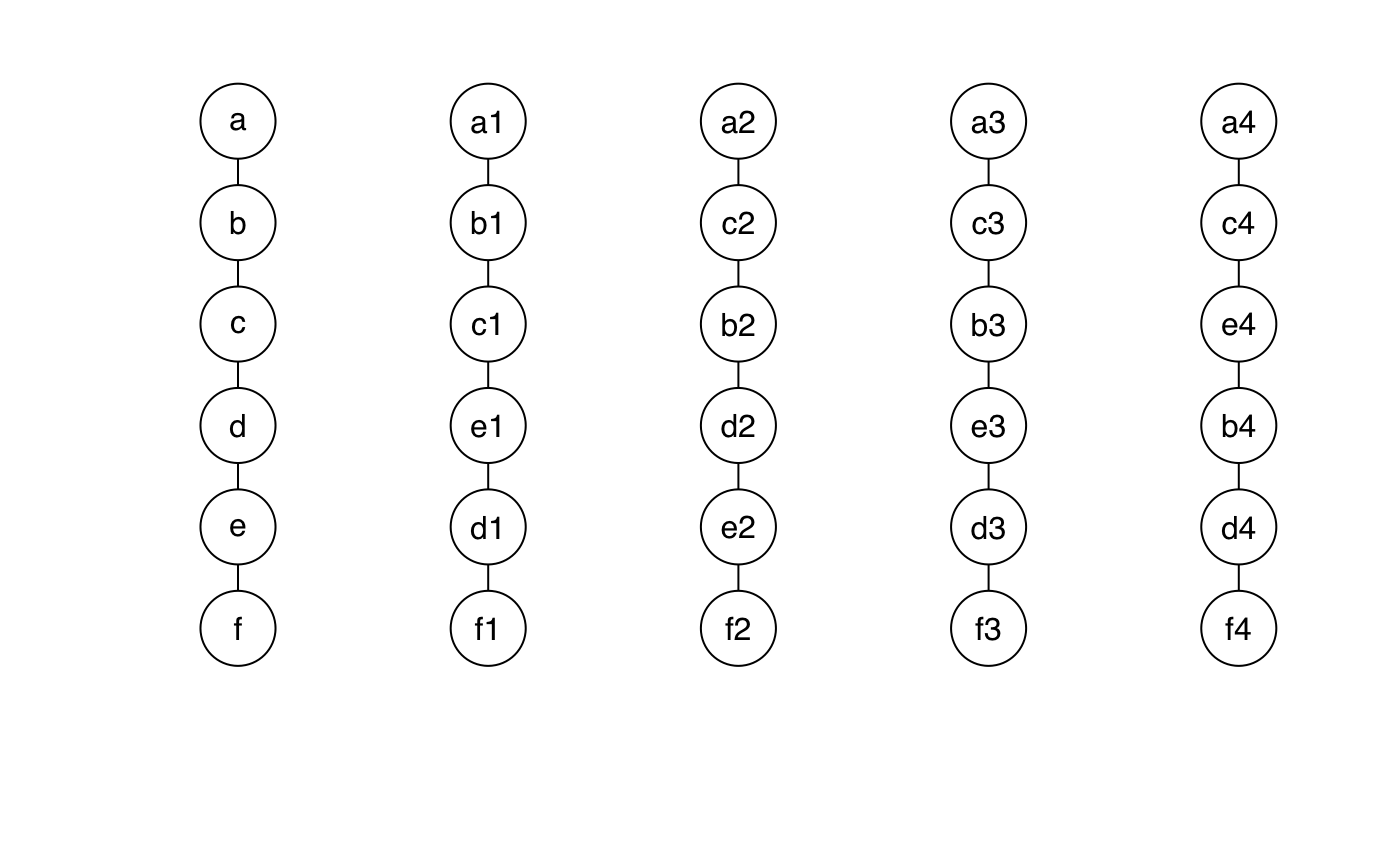
\includegraphics[width=10cm]{IMAGES/poset_13.png}
    \caption{Poset anticatena di catene.}
    \label{fig:roc}
\end{figure}

Il poset in questione è costituito da un anticatena di 5 catene che contano ognuna 6 elementi, per un totale di 30 elementi.
Questo poset, il quale in realtà non è poi cosi vasto e nemmeno troppo complesso, da un'idea del problema computazionale per la matrice MRP.
Il tempo di calcolo per ottenere tutte le estensioni lineari risulta $> 35 \;min.$, sulla macchina sopra citata.


Risulta quindi chiaro come nonostante lo studio per algoritmi sempre più efficienti per il calcolo della matrice MRP, non sia possibile procedere con l'approccio completo ed estrarre tutte le estensioni lineari. Anche con macchine più performanti il problema di tempistiche estreme rimane e il tempo di computazione tende ad esplodere con l'aumento di complessità delle strutture. L'approccio completo è quindi utilizzabile solo su poset molto banali e rimane escluso dai problemi reali. 

\section{Approccio campionario.}
Per poter aggirare il problema di tempistiche che l'approccio completo richiede per generare la MRP, è possibile ricorrere a processi di campionamento che stimino la matrice a partire da un sottoinsieme di estensioni lineari. L'algoritmo di campionamento utilizzato è l'algoritmo Bubley–Dyer \citep{bubley} il quale risulta ad oggi uno dei più efficienti disponibili in letteratura.


L'algoritmo è costruito in modo tale che la distribuzione asintotica del campionamento sia uniforme, questo fa si che nella pratica, dopo un certo numero (abbastanza elevato) di run dell'algoritmo, la probabilità di estrazione dall'insieme delle estensioni lineari diventi uniforme.


Utilizzando delle macchine con una potenza di calcolo standard, come ad esempio quella sopra citata, l'algoritmo permette di applicare la procedura di valutazione a poset con un massimo di alcune centinaia di profili, prima che il tempo di computazione esploda. Vediamo infatti da tabella (Tabella 5.2) come migliorino i tempi di sui poset rispetto all'approccio completo.

\begin{table}[H]
\centering
	\begin{tabular}{l c}
	& Tempo di calcolo & Poset \\
	\hline
	a & 0.01 sec.  \\
	b & 0.01 sec.  \\
	c & 0.06 sec. \\
	d & 0.09 sec. \\
	\hline
	\end{tabular}
\caption{Tempistiche di estrazione delle estensioni lineari con l'approccio campionario.\label{t:table}}
\end{table}

Risulta immediatamente visibile come il tempo di calcolo sia estremamente più breve con questo approccio. Si riporta inoltre come, usando l'algoritmo Bubley–Dyer per il poset in Figura 12 si passi da un tempo di calcolo superiore a $35 \;min.$ ad un run che dura $3.96 \; sec.$. 


Tuttavia anche questo approccio presenta dei punti deboli. Capita spesso nei poset che ci si trova davanti avendo a che fare con problemi reali sono più ampi di quelli usati come esempio. Come accennato in precedenza anche questo algoritmo tende a rallentarsi estremamente al crescere della complessità delle strutture ed in questi casi, la procedura di campionamento delle estensioni lineari soffre di problemi computazionali e non può essere messa in atto facilmente.


Per dare un'idea della persistenza del problema si fa riferimento alla tabella (Tabella 5.3) usata \citep{fattore2018}, dove attraverso una formula per determinare il numero di run necessario per arrivare ad avere una distribuzione uniforme (dato un errore). La tabella riporta il numero di run per alcuni poset della famiglia $2^k$.

\begin{table}[H]
\centering
	\begin{tabular}{l c c}
	& Numero elementi & Run & Poset \\
	\hline
	$2^4$ & 16 & 3,359,977\\
	$2^5$ & 32 & 123,534,1006\\
	$2^6$ & 64 & 4,581,459,610\\
	$2^7$ & 128 & 168,568,776,870\\
	\hline
	\end{tabular}
\caption{Numero di run necessari per l'uniformità.\label{t:table}}
\end{table}

Risulta chiaramente intuibile come calcoli di questa portata non siano attuabili da macchine standard. Come detto in precedenza, nonostante il miglioramento di questo approccio, il problema computazionale persiste.


Un altro problema che può emergere utilizzando un approccio campionario è quello della gestione delle simmetrie. Nel caso in cui un poset possieda delle simmetrie, capita che gli elementi in questione abbiano fra loro il punteggio della MRP pari a 0.5, tuttavia, dato che con questo approccio si estrae solo un sottoinsieme di tutte le estensioni lineari possibili, potrebbe risultare che i punteggi della MRP non siano entrambe 0.5 ma diversi. Questo fa si che due elementi, in realtà equivalenti e che nel ranking dovrebbero finire pari-merito con lo stesso score, nella pratica vengano ordinati. Per meglio specificare il problema appena visto, si dice che usando le procedure di campionamento, per approssimare la MRP, può entrare in conflitto con la proprietà di simmetria, creando un ordinamento artificiale.
\\~\\
In conclusione, nonostante lo sforzo continuo per adottare algoritmi sempre più efficienti, risulta comunque chiaro come sia necessario un cambio di approccio per poter risolvere il problema computazionale. Come si è visto, al crescere degli elementi nei poset il numero di estensioni lineari esplode, dunque gli approcci standard, per la risoluzione del problema computazionale della MRP, sono utilizzabili solamente in casistiche di poset contenuti. Dato che problema computazionale risulta al momento ancora irrisolvibile, ci si interroga sull'esistenza di una possibile soluzione alternativa per generare dei ranking da dati ordinali multi-variati.

\chapter{Q: matrice down-sets}
Fino a questo momento si è presa in rassegna la struttura dei sistemi parzialmente ordinati e si è visto come nella teoria siano strumenti efficaci per creare dei ranking ma come collassino nella pratica sotto problemi computazionali. I problemi visti fino a questo momento fanno capire chiaramente come sia necessario un cambio di approccio al fine di ottenere dei ranking in tempi computazionali accettabili. A questo fine viene proposta e valutata una matrice sostitutiva alla MRP, con proprietà diverse ma che si pensa possa portare a dei ranking paragonabili.


Prima di poter introdurre adeguatamente la matrice in questione è necessario definire alcune sotto-strutture dei poset, sulle quali si basa l'idea e la costruzione del nuovo approccio.
La struttura in questione è il \textit{down-set}. Per completezza (e per necessità in seguito) viene definita anche la struttura "opposta", ovvero l'\textit{up-set}.

\begin{definition}[Down-set]
Sia $A$ un insieme su cui è vale una relazione di ordine parziale $\unlhd$, allora il sottoinsieme $D \subset A$ definito come $D=\{x\in A:x\unlhd d\}$ è un down-set generato da $d$.\\
Allora un down-set $D \in A$ soddisfa che $x\unlhd y\in D\Rightarrow x\in D$.
\end{definition}

Di fatto il down-set è un sottoinsieme di elementi chiusi verso il basso. Un down-set può essere generato da più elementi, al patto che siano incomparabili, questo fa si che l'anticatena di elementi incomparabili che genera il sottoinsieme definisca un bordo superiore.

Si definisce prima l'elemento che genera il sottoinsieme.

\begin{definition}[Elemento generante del down-set]
Se $D$ è un down-set del poset $(A,\unlhd)$ allora gli elementi generanti del down-set sono $\uparrow d=\{d\in A:x\in D\unlhd d\}$. Gli elementi generanti sono per definizione incomparabili tra di loro e per questo formano un anticatena. Inoltre $\uparrow d\in D$.
\end{definition}

Esistono due definizioni alternative, una in cui l'elemento generante fa parte del down-set e una in cui non ne fa parte. Per i fini dello studio si è preferita la definizione che comprende anche l'elemento generante nel down-set, anche se va precisato che non ci sarebbero state differenze sostanziali nell'altro caso.
Partendo ora dalla definizione di questi elementi risulta chiaro come i down-set siano dotati di un bordo superiore, creato dall'anticatena degli elementi generanti.

\begin{definition}[Bordo superiore]
Dato il poset $(A,\unlhd)$ e il down-set $D\subset A$, allora, il bordo superiore del down-set è l'insieme $X^{\uparrow}=\bigcup_{d\in D} \uparrow d$, ovvero l'insieme contenente l'anticatena degli elementi generanti.
\end{definition}

Tutte le definizione fornite fino ad ora valgono in maniera opposta per l'\textit{up-set}, il quale è un sottoinsieme di elementi chiusi verso l’alto, per questo motivo viene fornita solamente la definizione generale di questo sottoinsieme.

\begin{definition}[Up-set]
Sia $A$ un insieme su cui è vale una relazione di ordine parziale $\unlhd$, allora il sottoinsieme $U \subset A$ definito come $U=\{x\in A:u\unlhd x\}$ è un up-set generato da $u$.\\
Allora l'up-set $U \in A$ soddisfa che $y\in U\unlhd x\Rightarrow x\in U$.
Inoltre $\downarrow u$ è l'elemento generante dell'up-set, e $X^{\downarrow}$ è il bordo inferiore.
\end{definition}

Per meglio poter comprendere le sotto strutture appena definite si riportano gli elementi nell'immagine (Figura 6.1), dove è possibile osservare oltre alle strutture i bordi superiore ed inferiore.

\begin{figure}[H]
    \centering
    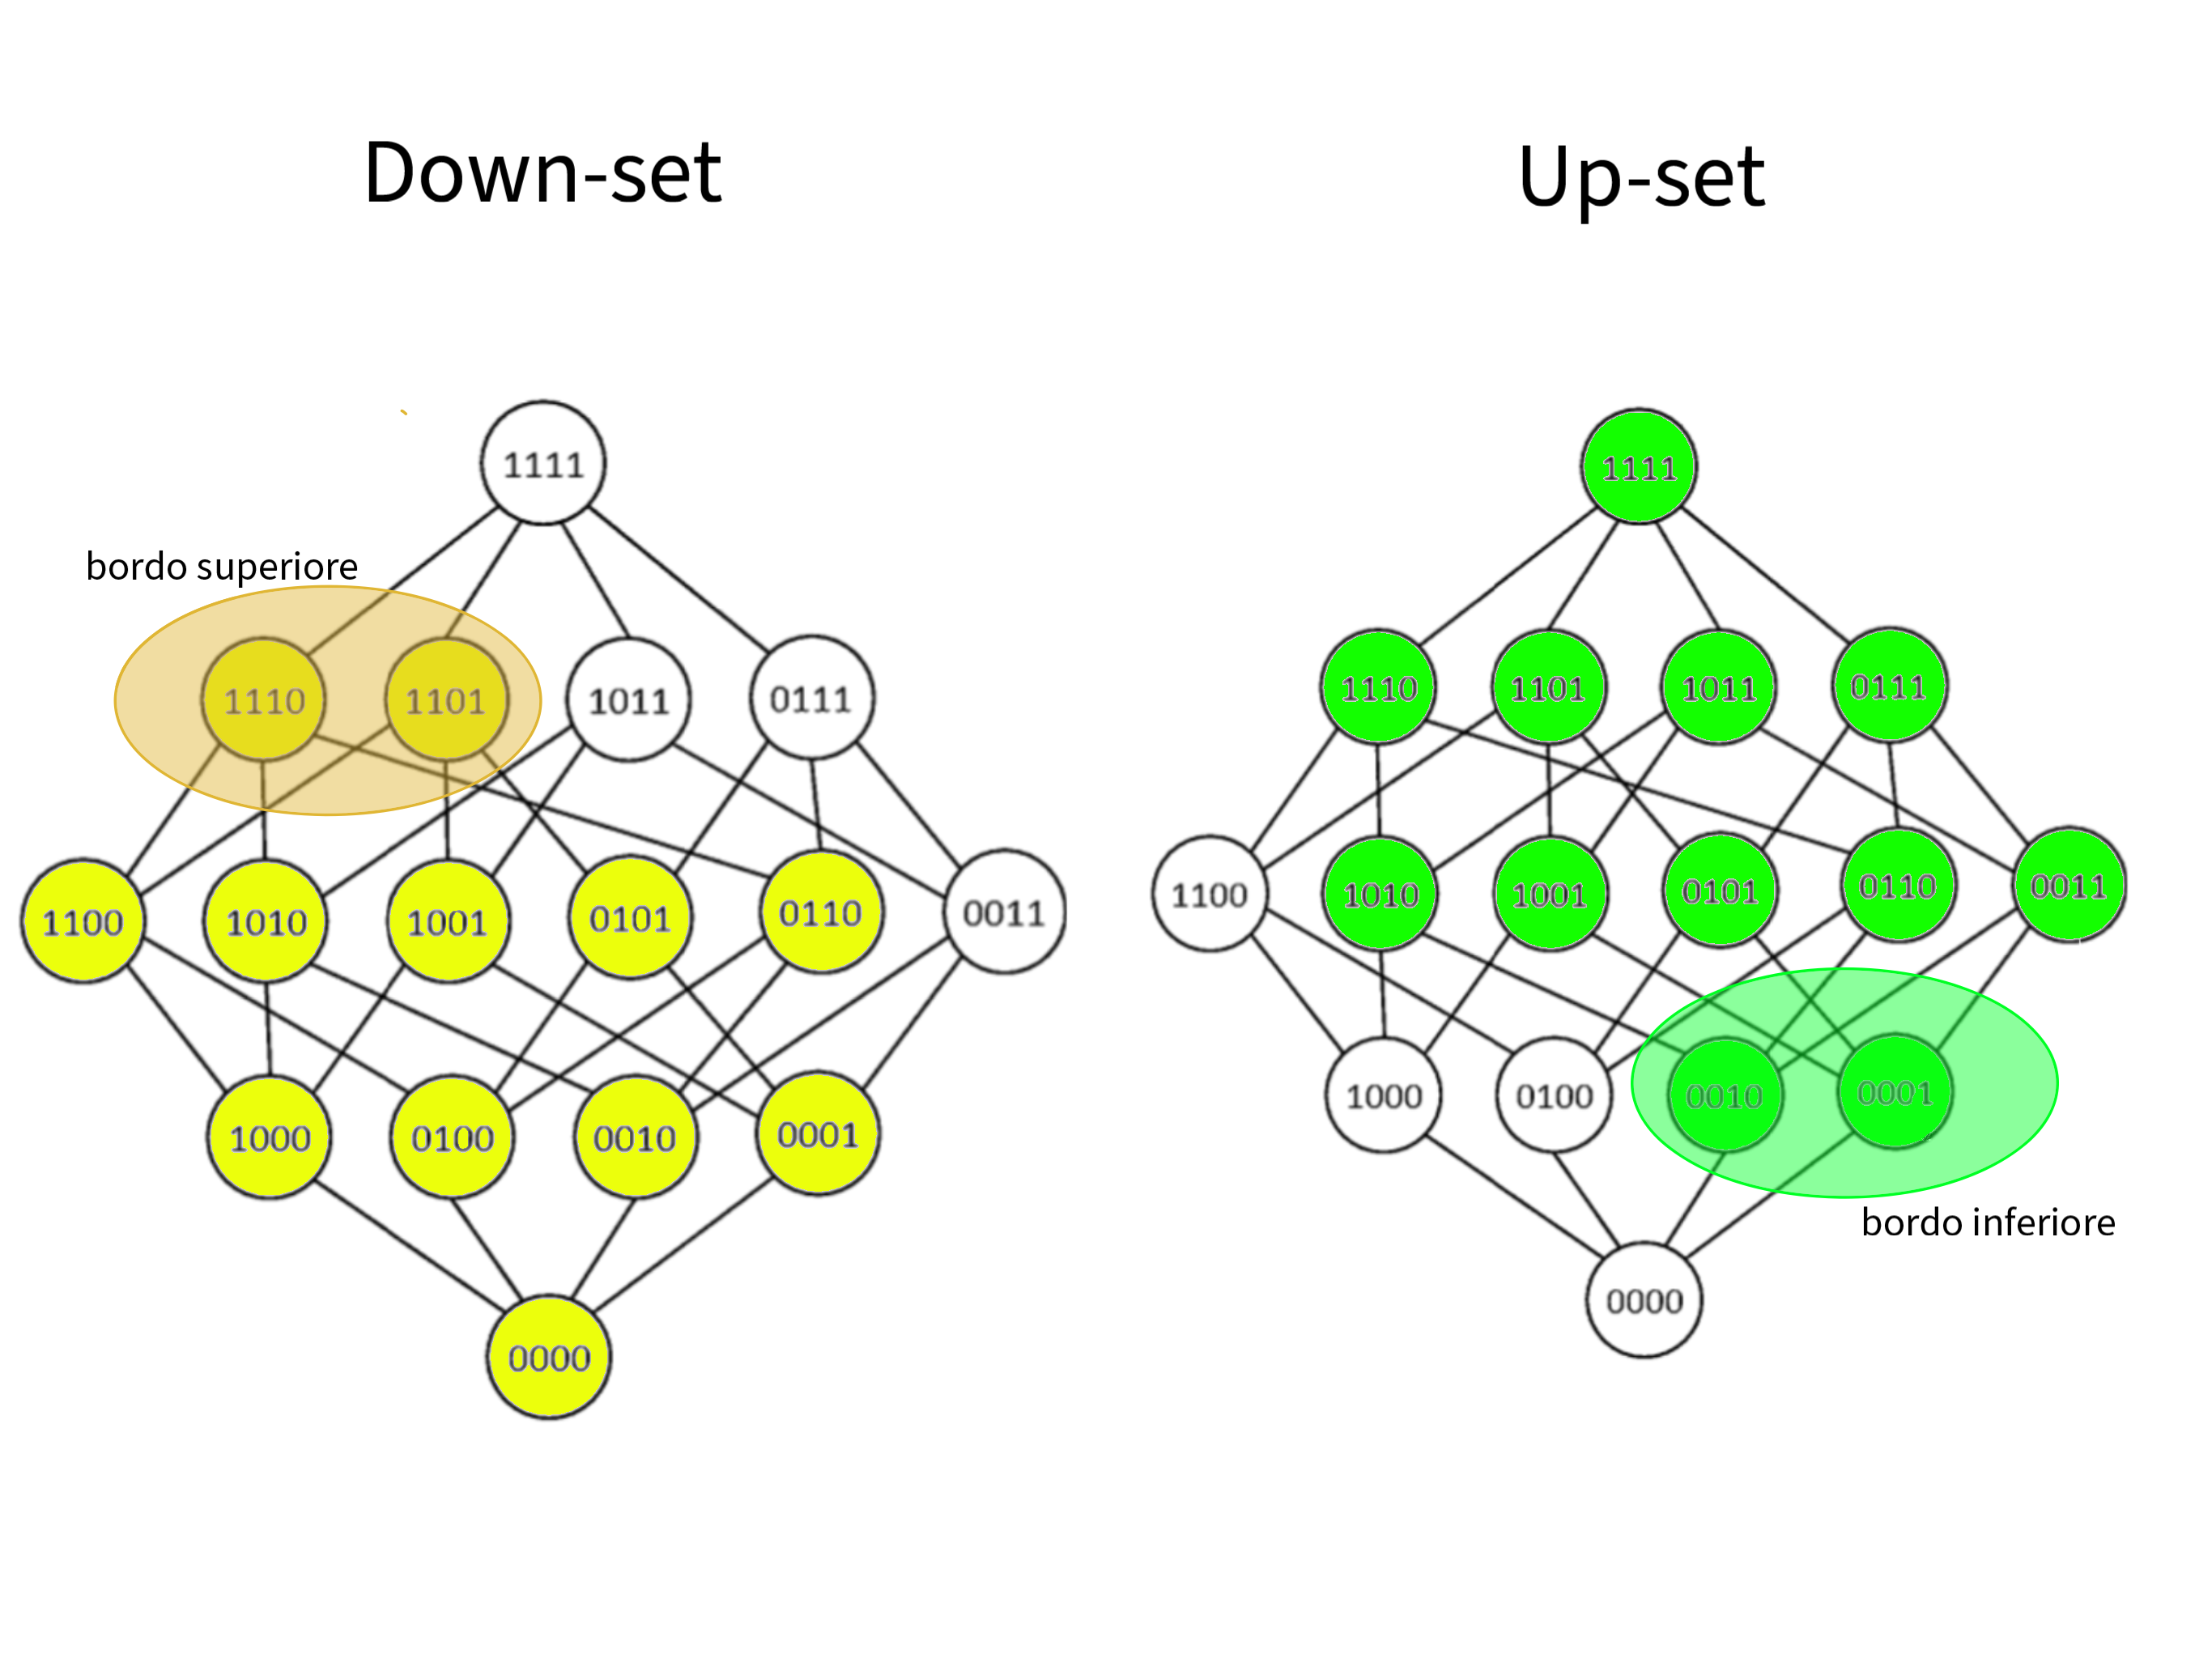
\includegraphics[width=10cm]{IMAGES/poset_14.png}
    \caption{Down-set e up-set con i relativi bordi.}
    \label{fig:roc}
\end{figure}
\\~\\
Avendo definito tutte le strutture necessarie, si procede ora con l'introduzione della matrice punta a sostituire la MRP nella creazione di ranking. L'idea di base parte dal fatto che gli elementi del poset che dominano di più rispetto ad altri avranno verosimilmente posizioni più alte nei ranking prodotti dalla MRP. Si ricorda ora che l'obbiettivo è riuscire ad emulare il più accuratamente possibile il sistema di ranking della MRP, il quale di per se sarebbe perfetto se non fosse così oneroso da calcolare. Viene per questo introdotta la matrice \textit{down-sets} (DS).

\paragraph{Matrice down-sets}
La matrice down-sets come detto in precedenza parte dall'idea che gli elementi che occupano le posizioni più elevate nel ranking siano quelli che dominano di più. Inoltre la matrice è costruita per essere facilmente calcolabile, i tempi di computazione sono paragonabili a quelli per le matrici di incidenza e di dominanza, quindi non esiste un problema computazionale. 


Indicando con $x_1, ..., x_n$ gli elementi dell'insieme $A$ sul quale viene definita la relazione d’ordine parziale $\unlhd$, la matrice di down-sets, che verrà indicata come $Q$ (per non confonderla con altre matrici), è una matrice $n\times n$ definita come segue:

\[Q_{ij} = \frac{|\{x_s\in A:x_s\unlhd x_i \land x_s\unlhd x_j\}|}{|\{x_s\in A:x_s\unlhd x_i\}|}.\]

Questo vuol dire che $Q_{ij}$ è dato dal numero di elementi che il down-set dell'elemento di riga condivide con il down-set dell'elemento di colonna fratto il numero di elementi del down-set dell'elemento di riga. In altre parole $Q_{ij}$ è la percentuale del down-set di $x_i$ contenuta nel down-set di $x_j$.


Si fa ora attenzione al fatto che se $x_i\unlhd x_j$, ovvero se l'elemento di colonna domina l'elemento di riga, chiaramente il down-set di quest'ultimo sarà contenuto interamente nel down-set del primo; questo implica che dove la matrice di dominanza $Z$ vale 1, anche la matrice DS varrà 1 e viceversa.
La facilità dei calcolo della nuova matrice dipende dal fatto che essa è facilmente derivabile a partire dalla matrice $Z$. Come si può notare, osservando una matrice di dominanza per colonna, si osservano i down-set generati dagli elementi per colonna. Questo fa si che gli elementi contenuti in tutti e due i down-set saranno gli elementi per entrambe le colonne la matrice $Z$ vale 1 e il numero di elementi del down-set sarà il numero di 1 nella colonna. Da questa relazione tra le due matrice deriva la formula per calcolare facilmente la matrice DS partendo dalla matrice $Z$.

\[Q_{ij} = \frac{|Z_{\cdot j}=1 \land Z_{\cdot i}=1|}{|Z_{\cdot i}=1|}.\]

Al contrario per ottenere la matrice di dominanza $Z$ da quella di down-sets $Q$ basta porre a 0 tutte le entrate diverse da 1.


Come ultima nota prestiamo attenzione sui tempi di computazione di questa nuova matrice. Le tempistiche di calcolo, come detto in precedenza e come intuibile dalla costruzione della matrice stessa, non sono distanti da quelle necessaire per le matrici $C$ e $Z$ dato che, per calcolarla, è semplicemente necessario un ciclo che prenda in rassegna le colonne di $Z$. Per precisione si riportano i tempi di computazione dei poset usati in precedenza (Figura 5.1).

\begin{table}[H]
\centering
	\begin{tabular}{l c}
	& Tempo di calcolo & Poset \\
	\hline
	a & 0.01 sec. \\
	b & 0.02 sec. \\
	c & 0.09 sec. \\
	d & 0.10 sec. \\
	\hline
	\end{tabular}
\caption{Tempistiche di estrazione della matrice down-sets.\label{t:table}}
\end{table}

Come ci si aspettava i tempi di calcolo sono molto contenuti. Inoltre anche la matrice per il poset in Figura 12 viene calcolata in tempistiche simili ($0.71\;sec.$). Si precisa che anche in poset con migliaia di elementi i tempi di calcolo sono brevi, diversamente che per la MRP che, con entrambi gli approcci, con numeri elevati di elementi fa esplodere il tempo computazionale.
Si intuisce come il problema di computazione non persista nella matrice $Q$, rimane ora il comprendere l'efficacia o meno del sistema di ranking che ne deriva e se esso possa effettivamente sostituire quello prodotto con la MRP.
\\~\\
Al fine di comprendere a pienamente la struttura della DS si riporta lo stesso poset usato come esempio per le altre matrici (Figura 2.5) e se ne osserva la matrice down-sets.

$Q=$
\begin{blockarray}{ccccccccc}
& a & b & c & d & e  \\
\begin{block}{c(ccccccccc)}
  a & 1 & 1/2 & 1/2 & 1/2 & 1/4 \\
  b & 2/3 & 1 & 1/3 & 2/3 & 1/3 \\
  c & 1 & 1/2 & 1 & 1/2 & 1/2 \\
  d & 1 & 1 & 1/2 & 1 & 1/2 \\
  e & 1 & 1 & 1 & 1 & 1 \\
\end{block}
\end{blockarray}

Si può osservare come la matrice DS contenga un'informazione maggiore rispetto alle matrici di dominanza e di incidenza, ci si domanda quindi se lo score che si ottiene da questa matrice possa portare a dei ranking solidi.


La procedura di score per ottenere il ranking, come viene ora esplicitato, non è dissimile da quella utilizzata per la matrice MRP usando l'average rank. Semplicemente si applica la decomposizione a valori singolari alla matrice $Q$, ottenendo così $Q=UDV^T$, come in precedenza prendendo l'autovettore della matrice DS relativo all'autovalore maggiore (ovvero la prima colonna di V), si definisce la funzione di scoring in modo che $s(x_i)=v_i$.


Si riporta ora in Tabella 6.2 il ranking estratto dal poset adoperando la nuova matrice proposta.

\begin{table}[H]
\centering
	\begin{tabular}{l c c}
	& Elementi & Score & Ranking \\
	\hline
    \ang{1} &	a &	0.5469472 \\		
    \ang{2} &	b &	0.4789603 \\		
    \ang{3} &	d &	0.4467444 \\		
    \ang{4} &	c &	0.4054582 \\		
    \ang{9} &	e &	0.3278244 \\		
    \hline
    \end{tabular}
    \caption{Ranking con score estratto usando la DS. \label{t:table}}
\end{table}

Il ranking ottenuto sembra funzionare, nei capitoli seguenti si descriveranno i comportamenti peculiari della matrice davanti a diverse strutture di poset e si valuterà in seguito l'efficacia di questa nuova procedura attraverso un confronto diretto con i ranking prodotti dalla MRP.

\chapter{Proprietà della matrice DS e confronto con la matrice MRP}
In questa sezione verrà affrontato il comportamento dei ranking prodotti dalla matrice DS. L'obiettivo finale è quello di testare l'efficacia o meno di questa matrice nel riuscire a produrrei dei ranking sensati e che non si discostino troppo da quelli prodotti dalla matrice MRP, i quali vengono presi come modello ideale. Ovviamente quello che ci si aspetta è che, essendo le due matrici costruite su informazioni diverse dei poset e avendo avendo informazioni intrinseche diverse, ci sia una qualche differenza nei ranking che si andranno a produrre. Lo scopo quindi è quello di valutare tale differenza e, nel caso la diversa logica di ordinamento della nuova matrice risulti "sensata", valutarne e annotarne le differenze, i comportamenti e le proprietà. Al fine di valutare la differenza tra i ranking che vengono prodotti dalle matrici si introducono due metriche di confronto, una numerica ed una visiva.
\\~\\
La prima delle due metriche proposte è il \textit{coefficiente di correlazione tra ranking di Kendall} o più semplicemente $\tau$ \texit{di Kendall}.

\begin{definition}[$\tau$ di Kendall]
Sia $(x_1,y_1), ...,(x_n,y_n)$ un insieme di osservazioni di due variabili casuali congiunte $X$ e $Y$, tale che tutti i valori $x_i$ e $y_i$ sono unici. Ogni coppia di osservazioni $(x_i,y_i)$ e $(x_j,y_j)$, dove $i<j$, sono dette \textit{concordanti} se concorde con l'ordinamento di $(x_i,x_j)$ e di $(y_i,y_j)$: questo vale se, valgono entrambe $x_i>x_j$ e $y_i>y_j$, o entrambe $x_i<x_j$ e $y_i<y_j$; altrimenti sono dette \texit{discordanti}.
Il $\tau$ di Kendall è definito come:
\[\tau = \frac{(\textrm{numero di coppie concordanti})-(\textrm{numero di coppie discordanti})}{\left( \begin{array}{c} n\\ 2 \end{array} \right)}.\]
Dove $\left( \begin{array}{c} n\\ 2 \end{array} \right)=\frac{n(n-1)}{2}$ è il coefficiente binomiale del numero di modi in cui è possibile estrarre due oggetti da $n$ oggetti.
\end{definition}

Quella appena fornita è la definizione base della metrica, in realtà ne esistono più versioni. La metrica base, riportata sopra, è chiamata \textit{tau-a}. Per gli scopi di comparazione, necessari per gli scopi di questa tesi, viene usata la metrica \textit{tau-b} (ne esiste una terza versione chiamata \textit{tau-c}, che non verrà riportata).

\begin{definition}[$\tau_b$]
La metrica tau-b, è una forma alternativa della metrica tau-a che prevede un aggiustamento per i valori pari merito (con stesso punteggio nel ranking). In modo uguale alla metrica base, anch'essa varia tra -1 e +1 e questi valori vengono interpretati in modo identico.
Il coefficiente tau-b è definito come:
\[\tau_b = \frac{n_c - n_d}{\sqrt{(n_0 - n_1)(n_0 - n_2)}},\]
dove:
\begin{enumerate}
  \item[] $n_0 = n(n-1)/2$
  \item[] $n_1 = \sum_i t_i(t_i -1)/2$
  \item[] $n_2 =\sum_j uj(uj-1)/2$
  \item[] $n_c = \text{Numero di coppie concordanti}$
  \item[] $n_d = \text{Numero di coppie discordanti}$
  \item[] $t_i = \text{Numero di valori pari merito nel gruppo $i$-esimo per la prima quantità}$
  \item[] $u_j = \text{Numero di valori pari merito nel gruppo $j$-esimo per la prima quantità}$
\end{enumerate}
\end{definition}

A partire da questo punto in avanti, si farà riferimento alla metrica tau-b chiamandola semplicemente \textit{tau}.
Nel nostro caso le coppie di variabili sono gli elementi in una determinata posizione nei ranking prodotti dalle matrici.
Essendo il denominatore il numero totali di combinazioni, il coefficiente varia nel range di $-1\leq \tau \geq 1$. L'interpretazione di questo coefficiente è che se i due ranking sono perfettamente coincidenti assume valore 1, se i due ranking sono perfettamente dissimili (uno è l'inverso dell'altro) assume valore -1. In aggiunta si riporta che il coefficiente assume valore 0 se i due ranking sono indipendenti, scenario che non dovrebbe succedere dato che, nonostante la diversa informazione racchiusa nelle matrici, il poset di partenza per gli ordinamenti rimane lo stesso.
\\~\\
La seconda metrica che viene introdotta, al fine di valutare le differenze tra i ranking prodotti dai due diversi approcci, consiste nella costruzione di un poset partendo dall'ordinamento prodotto dei ranking.
Prima di procedere alla spiegazione del funzionamento di questa metrica si definisce brevemente l'ordinamento prodotto.

\begin{definition}[Ordinamento prodotto]
Dati due ordinamenti $\unlhd_x$ e $\unlhd_i$, l'ordinamento prodotto è un ordinamento parziale del cartesiano, tale che: 
\[x_i\unlhd_x x_j \Leftrightarrow p_{s}(i)\unlhd_i p_{s}(j) \land \exists t:p_t(i) \lhd p_t(j),\]
per $p=1, ...,k$. Dove $\unlhd_x \subset \unlhd_i$ con $\unlhd_i$ rilevanza delle variabili o configurazione dei punteggi.
\end{definition}

Per questo motivo vale che tutti gli ordinamenti sono un sottoinsieme di quello prodotto.
Nel nostro caso l'ordinamento deriverà dalle posizioni del ranking, in modo che posizioni più elevate valgano di più e così facendo si estrae la metrica di confronto come illustrato di seguito.

Per mostrare il funzionamento di questa metrica vengono presi due ranking fittizi fatti sullo stesso poset.
\begin{table}[H]
\centering
	\begin{tabular}{l c c}
	& MRP & DS & Ranking \\
	\hline
    \ang{1} &	a &	b \\		
    \ang{2} &	b &	a \\		
    \ang{3} &	c &	c \\		
    \ang{4} &	d &	d \\		
    \hline
    \end{tabular}
\end{table}

Prendendo ora in esame solamente uno dei due ranking, ad esempio quello della MRP, si immagina un ordinamento prodotto che ne segua la logica, ovvero in questo caso $d\unlhd c \unlhd b \unlhd a$. In seguito si prende in rassegna il secondo ranking e si usa lo stesso procedimento, per ottenere in questo caso $d\unlhd c \unlhd a \unlhd b$. Una volta ottenuti i due ordinamenti li si confronta e si tengono solamente le dominanze comuni ad entrambi. Questo significa che elementi con dominanze che si contraddicono saranno incomparabili, in questo caso, dato che nel primo ranking $b \unlhd a$, mentre nel secondo $a \unlhd b$, ne consegue quindi che $a\parallel b$. Così facendo si definisce l'ordinamento prodotto $\unlhd_i$ sulla rilevanza degli elementi. In questo caso l'ordinamento prodotto è tale da avere le seguenti relazioni di dominanza: 
\begin{itemize}
    \item[] $c \unlhd a$
    \item[] $c \unlhd b$
    \item[] $d \unlhd c$
\end{itemize}

Da questo ordinamento prodotto si mappa il diagramma di Hasse relativo per comprendere la similarità tra i ranking.

\begin{figure}[H]
    \centering
    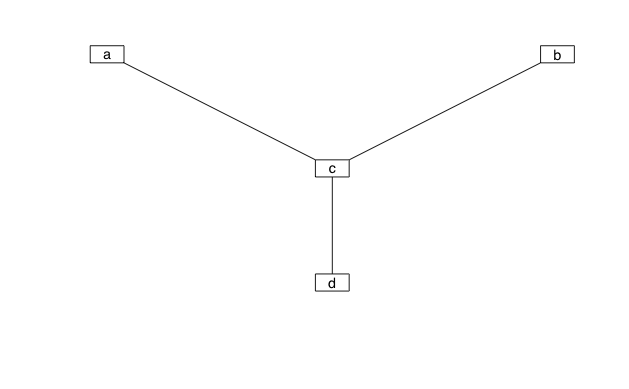
\includegraphics[width=10cm]{IMAGES/poset_15.png}
    \caption{Diagramma di Hasse dell'ordinamento prodotto.}
    \label{fig:roc}
\end{figure}

L'interpretazione di questa metriche è che, più il diagramma di Hasse è lineare (meno incomparabilità ci sono), più i ranking sono simili, al contrario più il diagramma si allontana da una forma lineare più i ranking sono diversi tra loro. Per poter distinguere il diagramma di Hasse dell'ordinamento prodotto dato dai due ranking da quello del poset di input, come da immagine gli elementi sono rappresentati in modo rettangolare al posto del classico cerchietto.


È necessario precisare, che a scopo puramente grafico, gli elementi che nel ranking hanno stessa posizione pari merito, nel diagramma di Hasse vengono comunque ordinati (in modo casuale), poiché lo scopo di questa metrica è quello di confronto tra i ranking e altrimenti si complicherebbe l'interpretazione visiva.
\\~\\
Avendo definito queste due utili metriche di confronto, che saranno fondamentali per la valutazione della DS, è ora possibile procedere nel prendere in rassegna le varie strutture dei poset e valutarne i comportamenti della matrice $Q$ e le differenze di produzione di ranking dalla matrice $M$.

\section{Gestione incomparabilità}
Come prima questione vediamo una differenza sostanziale tra i ranking generati dalla DS e quelli generati dalla MRP, ovvero la gestione delle incomparabilità. Per gestione delle incomparabilità si intende il modo di classificare quegli elementi che più degli altri sono affetti da incomparabilità.


Precedentemente si è visto come i ranking derivati dalla MRP abbiano la tendenza di posizionare gli elementi più incomparabili al centro della classifica, proprietà che rende di fatto necessaria la metrica score di incomparabilità al fine di riconoscere questi elementi.


Diversamente la matrice down-sets, per costruzione, tende ad attribuire punteggi di score bassi agli elementi con più incomparabilità, facendo si che essi "cadano" verso il fondo del ranking.

Si riportano ora degli esempi al fine di comprendere questo comportamento differente. Si vuole comunque precisare, che questa differenza che caratterizza il ranking della matrice $Q$ non viene vista come una differenza "negativa" (dato che precedentemente si è detto che il ranking ideale a cui si punta è quello della matrice MRP), quanto più una differenza strutturale che può aiutare ad individuarne quegli elementi più incomparabili in modo più veloce.
In generale, in qualunque posizione venga piazzato, un elemento fortemente incomparabile all'interno di un ranking risulta comunque una forzatura. La questione fondamentale è il riuscire ad individuare questi elementi per poterne valutare la posizione in maniera empirica.

\begin{figure}[H]
    \centering
    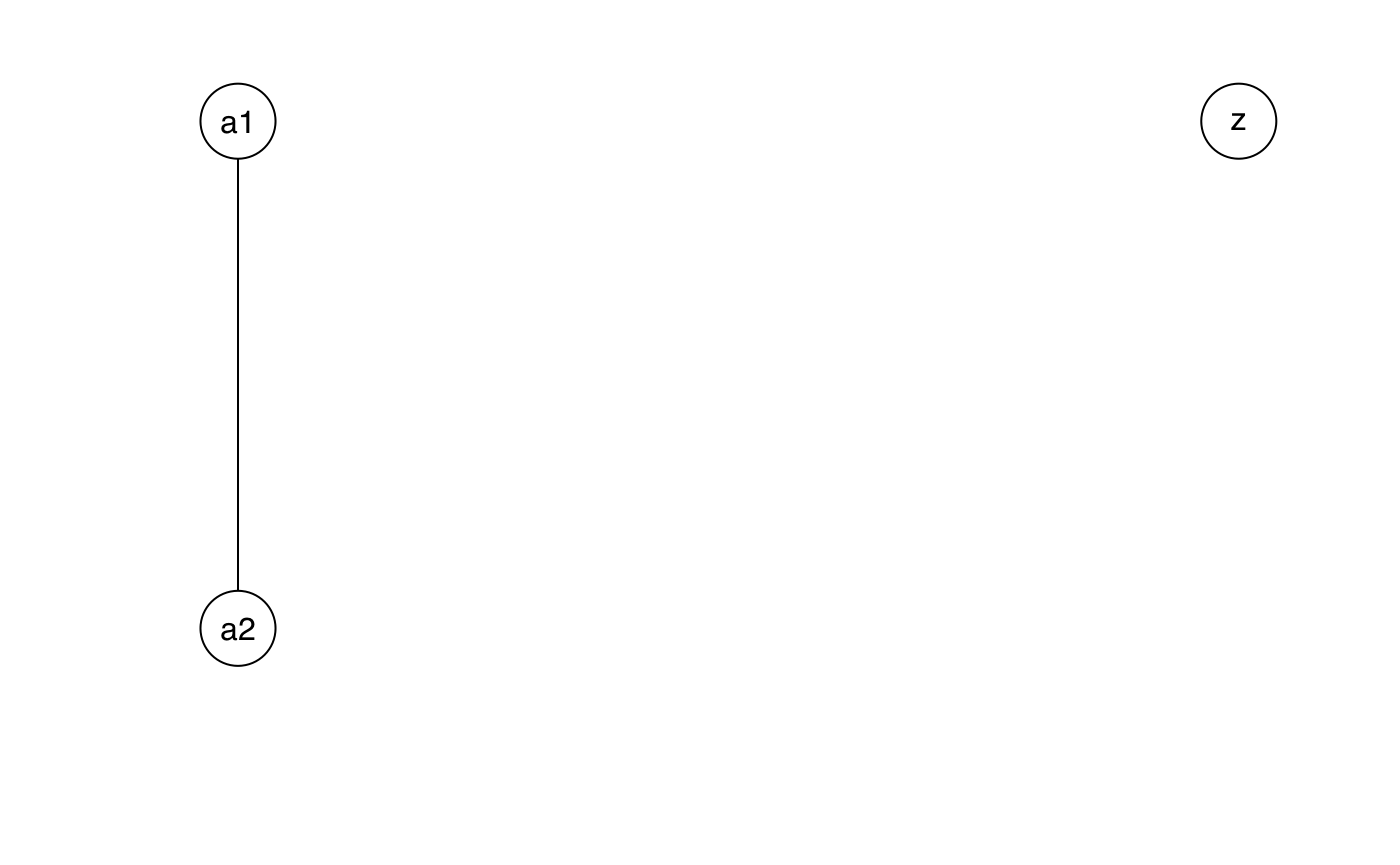
\includegraphics[width=10cm]{IMAGES/poset_1.png}
    \caption{Poset con incomparabilità.}
    \label{fig:roc}
\end{figure}

Osservando il poset (Figura 7.2), semplicemente composto da tre elementi di cui due comparabili ed un terzo totalmente incomparabile notiamo le differenze di comportamento nel ranking per i due approcci.

\begin{table}[H]
\centering
	\begin{tabular}{l c c c c}
	& Ranking MRP & Score MRP & Ranking DS & Score DS & Posizione \\
	\hline
	\ang{1} &  a1 & 0.7145692 & a1 & 0.7882054	 \\
	\ang{2}  & \textbf{z} & 0.5551806 & a2 & 0.6154122	 \\
	\ang{3} & a2 & 0.4256352 & \textbf{z} & 0.0000000	 \\
	\hline
	\end{tabular}
\caption{Ranking con score delle prodotti dalle due matrici $M$ e $Q$.\label{t:table}}
\end{table}

È possibile notare, come preannunciato, la differenza di posizionamento dell'elemento $z$. Lo score di questo elemento ottenuto dalla matrice $Q$ è 0, poiché, non essendo comparabile con nessun altro elemento non contiene il down-set di nessun elemento e non fa parte del down-set di nessun elemento; per questo motivo la colonna e la riga $z$ della matrice $Q$ sono composte solo da zeri (a parte un 1 dove per $Q_{zz}$). In realtà lo score di questo dell'elemento $z$ è nullo per un altro comportamento della matrice che verrà analizzato in seguito, tuttavia in questo frangente è utile visionare il comportamento in questo modo poiché comunque aiuta a comprendere come la matrice $Q$ classifica gli elementi poco comparabili.


Nonostante l'esempio appena fatto sia potente dal punto di vista esplicativo, al fine di comprendere il comportamento dei due apporci nel trattare elementi incomparabili, non è chiaro, fino ad ora, se questa caratteristica affligga o meno, in modo irreparabile, la somiglianza tra i due ranking. Per questo motivo si riporta (Figura 7.3) un poset leggermente più complesso, con tutti gli elementi caratterizzati da una comparabilità media,a parte per un elemento, il quale è poco comparabile con gli altri.

\begin{figure}[H]
    \centering
    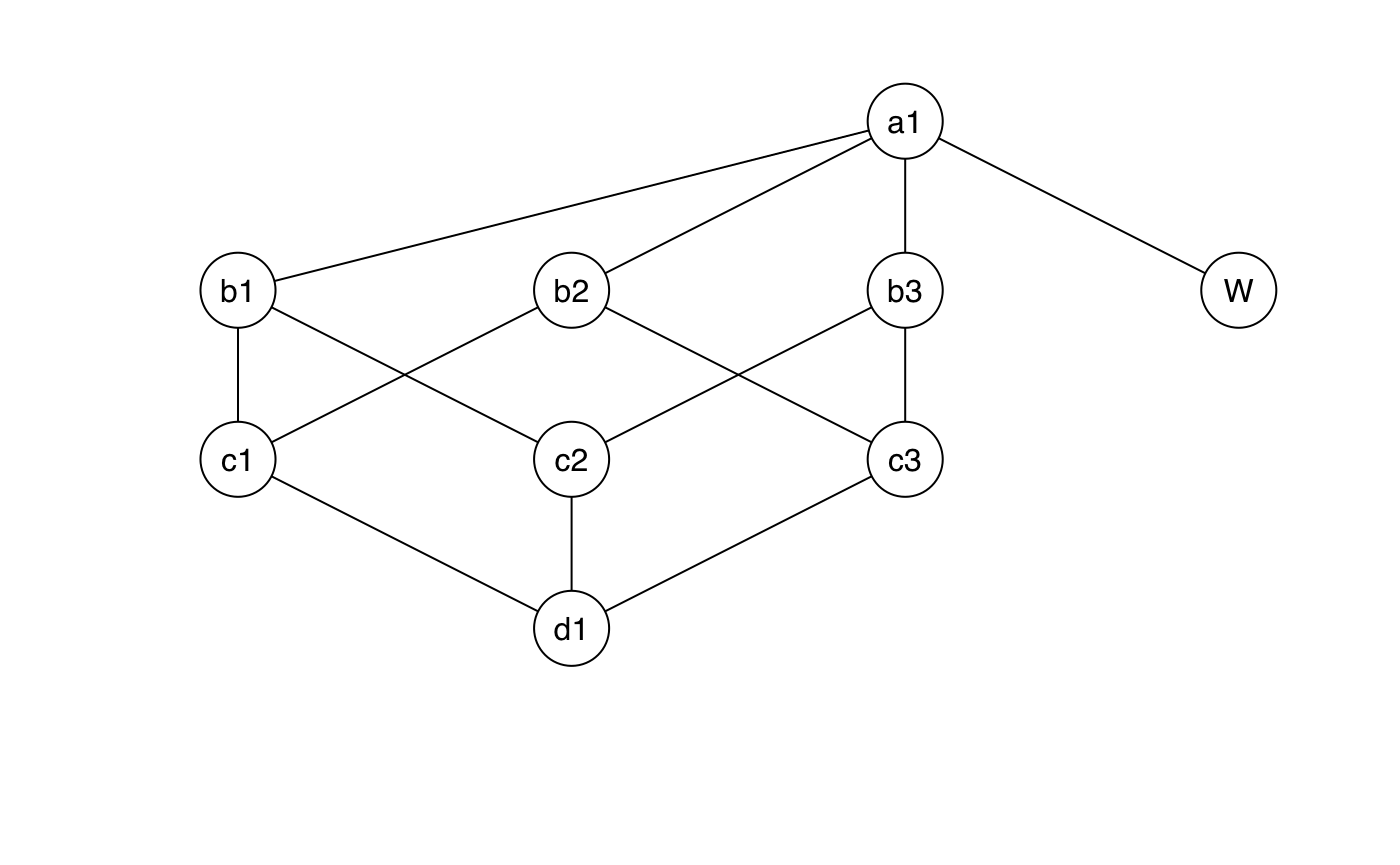
\includegraphics[width=12cm]{IMAGES/poset_2.png}
    \caption{Poset con elemento W meno comparabile.}
    \label{fig:roc}
\end{figure}

Si riportano ora (Tabella 7.2) come di consueto i due ranking estratti con i due approcci. È possibile notare come i due ordinamenti siano di fatto identici, escluso l'elemento $W$. In maniera empirica i due ranking sembrano molto simili, al fine di canonizzare questa idea si osservano ora le due metriche introdotte all'inizio di questo capitolo.

\begin{table}[H]
	\begin{minipage}{0.4\linewidth}
		\label{table:student}
		\centering
        \begin{tabular}{l c c}
         	& Ranking MRP & Ranking DS & Posizione \\
         	\hline
            \ang{1}|\ang{1} &	a1	& a1 \\		
            \ang{2}|\ang{2} &	b1	& b1 \\		
            \ang{2}|\ang{2} &	b2	& b2 \\		
            \ang{2}|\ang{2} &	b3	& b3 \\		
            \ang{3}|\ang{3} &	\textbf{W}	& c1 \\		
            \ang{4}|\ang{3} &	c1	& c2 \\		
            \ang{4}|\ang{3} &	c2	& c3 \\		
            \ang{4}|\ang{4} &	c3	& d1 \\		
            \ang{5}|\ang{5} &	d1	& \textbf{W} \\	
            \hline
		\end{tabular}
		\caption{Ranking a confronto. \label{t:table}}
	\end{minipage}\hfill
	\begin{minipage}{0.6\linewidth}
		\centering
		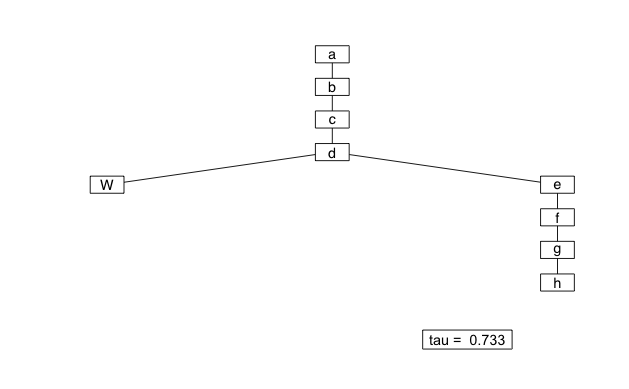
\includegraphics[width=10cm]{IMAGES/poset_2_05.png}
	\end{minipage}
\end{table}

Si più osservare dal grafico affiancato alla tabella come i due ranking abbiano un valore di $\tau = 0.733$, il quale è un valore abbastanza alto, considerando anche il fatto che il poset risultante dal confronto dei due ranking è quasi completamente, fatta eccezione per l'elemento $W$, una catena. Di fatto si intuisce come, se non fosse per quell'elemento particolarmente a sé stante, il ranking della matrice down-sets avrebbe replicato in maniera perfetta il ranking della matrice mutual ranking probability.


Si appunta che, come precisato in precedenza, il fatto che il ranking ottenuto con la DS posizioni gli elementi incomparabili diversamente da quanto fatto dalla MRP, non è una differenza "negativa", dato che questi elementi vanno valutati empiricamente. Quindi si può dire che fino a questo momento la matrice DS sembra promettente come alternativa alla MRP, tuttavia in poset più complessi questa differenza potrebbe accentuarsi. Si procederà ora nel valutare il comportamento dei ranking in altre situazioni e altre strutture di poset, al fine cercare di comprende a pieno le differenze e le caratteristiche dei ranking estratti con la DS.


\section{Poset con $C/I$ alto.}
Una volta osservato il comportamento della DS nel posizionare gli elementi, di fatto più problematici, all'interno dei ranking, si osserveranno da questo momento in avanti poset il più differenti possibili. In questo paragrafo si osservano i poset con alto $C/I$, il quale sarebbe una dicitura informale dove, $C$ indica il numero di comparabilità e $I$ il numero di incomparabilità. In questo caso quindi saranno poset con più comparabilità che incomparabilità, ovvero poset con un diagramma di Hasse allungato e stretto.


Il primo poset che si prende in rassegna è una catena, la quale è per antonomasia un poset con $C/I$ alto. Senza necessità di riportare né grafici del poset, né ranking e nemmeno grafici degli indicatori; si è osservato (come da risultato atteso) che indipendentemente dal numero di elementi il valore di tau è sempre 1, ovvero che il ranking estratto talla matrice $Q$ è identico a quello estratto dalla matrice $M$.


Vengono ora analizzati alcuni poset (Figura 7.4) più complessi rispetto a quelli analizzati fino a questo momento. I poset in questione sono stati scelti come esempi, per poter valutare se per quelli con tendenzialmente un numero di comparabilità più elevato rispetto al numero di incomparabilità la procedura di ranking sia o meno efficacie.

\begin{figure}[H]
  \centering
  \begin{minipage}[b]{0.4\textwidth}
    \includegraphics[width=8cm]{IMAGES/poset_22.png}
  \end{minipage}
  \hfill
  \begin{minipage}[b]{0.4\textwidth}
    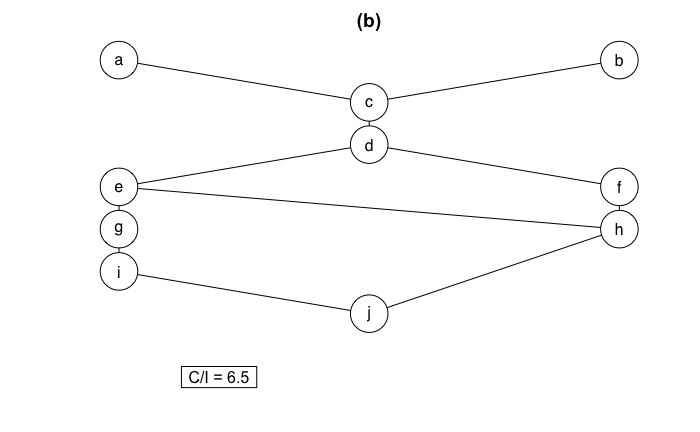
\includegraphics[width=8cm]{IMAGES/poset_18.png}
  \end{minipage}
  \hfill
  \begin{minipage}[b]{0.4\textwidth}
    \includegraphics[width=8cm]{IMAGES/poset_19.png}
  \end{minipage}
  \hfill
  \begin{minipage}[b]{0.4\textwidth}
    \includegraphics[width=8cm]{IMAGES/poset_21.png}
  \end{minipage}
  \caption{Quattro poset (a, b, c, d) con relativo $C/I$.}
\end{figure}

È possibile notare come i poset in questione (nonostante in figura sembrino abbastanza allargati) abbiano tutti gli elementi molto comparabili tra di loro, il che rende teoricamente più difficile che i ranking fatti usando le due procedure siano particolarmente diversi, dato che le "indecisioni" sui ranking avvengono a livello delle incomparabilità, come si è potuto intuire anche dall'esempio della catena. L'alta comparabilità degli elementi all'interno di questi poset esemplificativi è confermata dal fatto che il rapporto $C/I$ è sempre abbastanza alto, e non scende sotto 6.


Vengono ora riportati i grafici (Figura 7.5) relativi agli indicatori, per comprendere se i ranking prodotti dalla DS siano validi o meno. In questa fase ci si aspetta che i ranking prodotti con i due diversi approcci non siano così dissimili tra loro, dato che il numero di comparabilità è alto.

\begin{figure}[H]
  \centering
  \begin{minipage}[b]{0.4\textwidth}
    \includegraphics[width=8cm]{IMAGES/poset_22_05.png}
  \end{minipage}
  \hfill
  \begin{minipage}[b]{0.4\textwidth}
    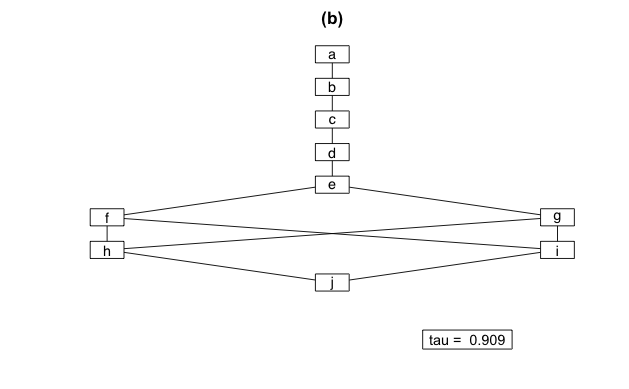
\includegraphics[width=8cm]{IMAGES/poset_18_05.png}
  \end{minipage}
  \hfill
  \begin{minipage}[b]{0.4\textwidth}
    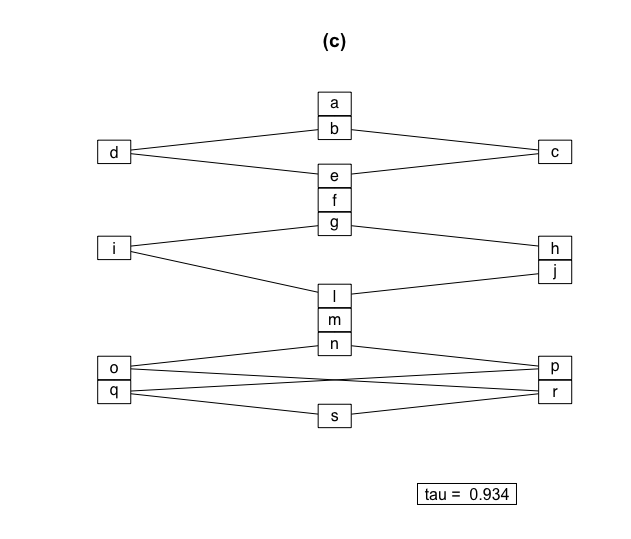
\includegraphics[width=8cm]{IMAGES/poset_19_05.png}
  \end{minipage}
  \hfill
  \begin{minipage}[b]{0.4\textwidth}
    \includegraphics[width=8cm]{IMAGES/poset_21_05.png}
  \end{minipage}
  \caption{Metrica grafica di comparazione e tau per comparare i due ranking DS e MRP dei poset (a, b, c, d).}
\end{figure}

Prendendo ora in rassegna i grafici si nota in generale come tau sia sempre molto elevata, con un valore comunque vicino a 0.9. Alcune visualizzazioni grafiche di similarità tra ranking, a prima occhiata, sembrano confuse (in modo particolare la figura d), viene quindi spontaneo chiedersi come mai nonostante questa "confusione" il valore di tau sia così alto. Di fatto, osservando più attentamente, i grafici aiutano a comprendere come i ranking siano in realtà simili e le differenze riscontrate corrispondo di fatto a semplici inversione di elementi, che, comunque, risultano vicini in entrambe i ranking. Il punto fondamentale è che in tutte e quatto le figure si vede chiaramente che lo scheletro del ranking è lo stesso, nonostante le differenze che produce l'estrazione dalle due matrici diverse. Questo tipo di differenze, sebbene siano doverose da riportare, corrispondono di fatto ad una minima variazione nel senso dell'intero ranking estratto da $Q$ al posto che da $M$.


Si vuole portare ora l'attenzione su come sembri che ci sia una tendenza che in qualche modo lega la relazione tra il numero di comparabilità e di incomparabilità e il valore di tau. Quella appena riportata è solamente un'impressione, nel caso dovesse persistere questa tendenza con i poset analizzati in seguito verrà presa in considerazione con più attenzione.


In generale sembra che il ranking ottenuto dalla matrice DS riproduca in modo abbastanza accurato e soprattutto conservi la struttura di base del ranking estratto dalla matrice MRP per quanto riguarda i poset con un rapporto di $C/I$ abbastanza elevato.


\section{Poset con $C/I$ basso.}
Si vuole ora osservare quei poset caratterizzati da un rapporto di comparabilità e incomparabilità basso, ovvero con un numero di incomparabilità più elevato rispetto ai poset precedenti. Essendo, quelli che verranno esposti, poset con un valore $C/I$ basso, i diagrammi di Hasse relativi saranno "opposti" a quelli del paragrafo precedente, con una forma larga e poco allungata. Il risultato che si attende è riscontrare una similarità più contenuta tra i due ranking, essendo gli elementi che compongono questi poset più incomparabili tra loro rispetto ai poset precedentemente visti. 


È doveroso precisare che non è stato possibile paragonare i ranking con un valore di $C/I$ più basso ma con lo stesso numero di elementi, dato che il tempo di estrazione della MRP sarebbe esploso. Si può immaginare come, quando sono presenti più incomparabilità (mantenendo lo stesso numero di elementi) le differenze nei ranking tendano ad accentuarsi. Questa idea verrà poi confermata dagli esempi riportati, comunque rimane un comportamento atteso.


Si riportano ora i poset (Figura 7.6) per tentare di comprendere le performance della DS con un numero di incomparabilità "elevato".

\begin{figure}[H]
  \centering
  \begin{minipage}[b]{0.4\textwidth}
    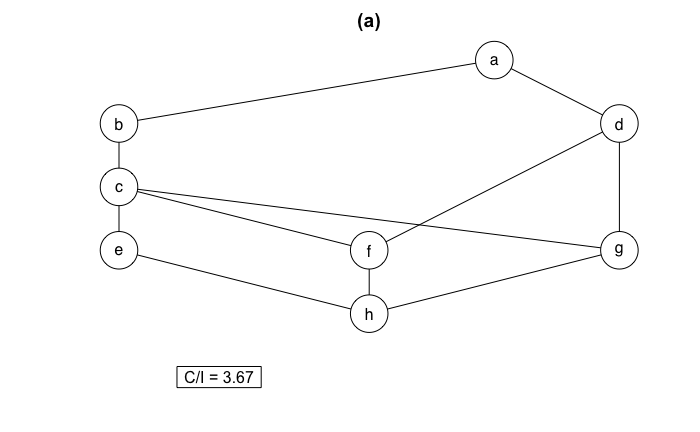
\includegraphics[width=8cm]{IMAGES/poset_17.png}
  \end{minipage}
  \hfill
  \begin{minipage}[b]{0.4\textwidth}
    \includegraphics[width=8cm]{IMAGES/poset_23.png}
  \end{minipage}
  \hfill
  \begin{minipage}[b]{0.4\textwidth}
    \includegraphics[width=8cm]{IMAGES/poset_24.png}
  \end{minipage}
  \hfill
  \begin{minipage}[b]{0.4\textwidth}
    \includegraphics[width=8cm]{IMAGES/poset_20.png}
  \end{minipage}
  \caption{Quattro poset (a, b, c, d) con relativo $C/I$.}
\end{figure}

Considerando i valori di $C/I$, sempre inferiori a 4, risulta chiara la forte incomparabilità degli elementi all'interno dei poset, fatto che, come detto prima, ci si aspetta porti ad un'accentuazione delle differenze dei ranking risultanti.


Vengono ora riportati i grafici (Figura 7.7) relativi agli indicatori, per poter capire se l'estrazione del ranking dalla matrice DS rimanga valida anche all'aumento di incomparabilità. 

\begin{figure}[H]
  \centering
  \begin{minipage}[b]{0.4\textwidth}
    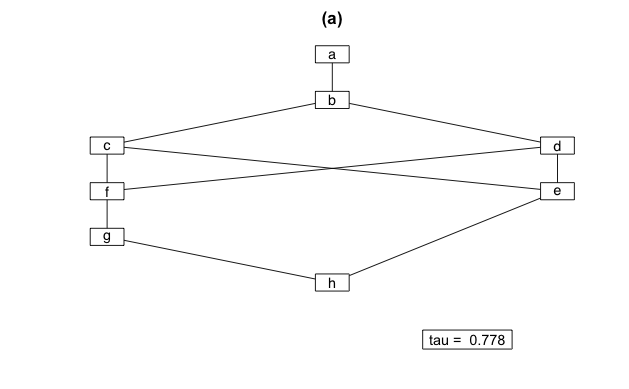
\includegraphics[width=8cm]{IMAGES/poset_17_05.png}
  \end{minipage}
  \hfill
  \begin{minipage}[b]{0.4\textwidth}
    \includegraphics[width=8cm]{IMAGES/poset_23_05.png}
  \end{minipage}
  \hfill
  \begin{minipage}[b]{0.4\textwidth}
    \includegraphics[width=8cm]{IMAGES/poset_24_05.png}
  \end{minipage}
  \hfill
  \begin{minipage}[b]{0.4\textwidth}
    \includegraphics[width=8cm]{IMAGES/poset_20_05.png}
  \end{minipage}
  \caption{Metrica grafica di comparazione e tau per comparare i due ranking DS e MRP dei poset (a, b, c, d).}
\end{figure}

Come da risultato atteso si è riscontrato un abbassamento dei tau, rispetto a quelli misurati per i poset precedenti, tuttavia i valori rimangono ancora abbastanza elevati, tendenzialmente superiori a 0.75. Questo significa che nonostante l'aumento delle incomparabilità le differenze tra i ranking non si sono accentuate più di tanto, rimanendo di fatto simili. 


Osservando ora i diagrammi di Hasse salta subito all'occhio come, rispetto a prima, i grafici siano più confusionari e come la struttura di fondo sia più difficile da intravedere. Ovviamente più elementi sono presenti più il diagramma di Hasse è differente da una catena, ma come in precedenza la maggior parte delle differenze tra i due ranking consiste semplicemente in inversioni di coppie e, in generale, vale che gli elementi non differiscono di più di tre posizioni tra un ordinamento e l'altro.


Nonostante le differenze presenti comunque, anche se come detto con più difficoltà, è sempre individuabile uno scheletro di fondo comune per i due ranking. La presenza appunto di questo scheletro fa ben sperare nella validità della matrice DS. Il riuscire a mantenere una struttura di fondo uguale tra i due ranking è più di impatto rispetto alle differenze superficiali.


La sensazione riportata nel capitolo precedente, secondo la quale il valore di tau sarebbe legato in qualche modo al rapporto $C/I$, viene in pratica smentita dal fatto che il poset c nonostante abbia il rapporto di comparabilità e incomparabilità più basso abbia il valore di tau più alto rispetto ai quattro poset. Nonostante questa considerazione però si può continuare a sostenere che comunque esista una tendenza alla differenziazione dei ranking con l'aumento di incomparabilità.


In conclusione nonostante il calo, atteso, di similarità i valori di tau rimangono comunque elevati e la struttura di fondo rimane sempre identificabile.

\section{Poset booleani}
In questo paragrafo verranno testate, come di consueto, le performance e i comportamenti dei ranking estratti dalla matrice down-sets, questa volta però senza valutare poset generati "casualmente" come in precedenza, ma utilizzando poset provenienti dalla famiglia dei poset booleani. I poset di questa famiglia sono già stati presentati nel capitolo 5 e la famiglia è chiamata anche $2^k$. In particolare si osservano i poset $2^2$, $2^3$ e $2^4$, i quali sono stati riportati come a, b, c nella Figura 5.1.


La particolarità che si riscontra con i poset appartenenti a questa famiglia è che, nonostante abbiano un rapporto di comparabilità su incomparabilità a volte estremamente basso, come nel caso di $2^3$ dove $C/I=65/55=1.18$, il ranking estratto dalla DS è identico a quello estratto dalla MRP, risultando in un tau di 1 e in un grafico di comparazione che consiste in una catena. Questo comportamento si verifica per tutti i poset booleani.


Questo risultato, disatteso per i ragionamenti fatti fino ad ora, smentisce la teoria secondo la quale il valore di tau, o comunque la similarità dei ranking fatti con i due diversi approcci, fosse in qualche modo legata al valore del rapporto $C/I$. Il motivo per cui DS ha delle performance cosi alte su questo tipo di poset si può ricercare nella struttura stessa di questi ultimi. 

\begin{figure}[H]
    \centering
    \includegraphics[width=10cm]{IMAGES/poset_25.png}
    \caption{Poset $2^3$ con elementi pari merito raggruppati.}
    \label{fig:roc}
\end{figure}

Come è possibile vederne un esempio dall'immagine (Figura 7.8), i poset booleani sono costruiti in modo da formare fasce di elementi tra loro incomparabili ma, che per il senso generale del ranking che ne verrà prodotto, saranno classificati pari merito agli elementi lungo la stessa fascia. Quello che di fatto succede è che gli elementi lungo la fascia sono interscambiabili e nella costruzione della MRP le colonne identificative degli elementi sulla stessa fascia sono costruite in modo da avere esattamente gli stessi valori ma in diverse posizioni. Lo stesso risultato di fatto viene raggiunto anche dalla DS, poiché gli elementi della stessa fascia hanno il down-set con le stesse identiche caratteristiche e tutti i down-set provenienti dalla stesa fascia interagiscono tra di loro in modo uguale, questo fa si che il ranking prodotto sia per fasce di elementi pari merito e quindi identico a quello estratto dalla MRP.


Per concludere il paragrafo, nonostante si sia dovuta abbandonare l'ipotesi secondo la quale i valori $C/I$ e tau fossero strettamente legati, si è sperimentato (non è provato matematicamente in nessun modo) come sembri che la matrice $Q$ sia la perfetta alternativa per l'estrazione di ranking da poset booleani.

\section{Poset disgiunti.}
In questo capitolo vengono presi in considerazione i poset disgiunti, ovvero quei sistemi parzialmente ordinati che consistono in tutto e per tutto in due sotto sistemi non comunicanti. In questi casi particolari sono risultati necessari, al fine di poter "correggere" alcuni comportamenti disattesi nella costruzione della matrice down-sets e nella successiva estrazione del ranking, alcune accortezze che facciano tornare dei risultati sensati.
Al fine di poter comprendere al meglio il tipo di poset in questione si riporta un esempio in Figura 7.9.

\begin{figure}[H]
    \centering
    \includegraphics[width=10cm]{IMAGES/poset_26.png}
    \caption{Poset disgiunto formato da due poset incomparabili.}
    \label{fig:roc}
\end{figure}

Il problema per questo tipo di poset è duplice, poiché l'essere disgiunti aumenta di molto il numero delle estensioni lineari e questo fa si che, ad esempio per il poset appena citato, computare la MRP sia troppo oneroso. Per il motivo appena visto si è scelto di mostrare il peculiare comportamento della matrice $Q$ su poset meno complessi, così da poter attuare ugualmente il confronto con la MRP per valutare le performance.

Si vuyole ora prendere in considerazione il poset in Figura 7.10, il quale è formato da un insieme di elementi comparabili tra loro, che va da $a$ ad $f$, e altri due elementi comparabili tra loro ma incomparabili con tutti gli altri, ovvero $h$ ed $i$.

\begin{figure}[H]
    \centering
    \includegraphics[width=10cm]{IMAGES/poset_27.png}
    \caption{Poset disgiunto formato da due poset incomparabili.}
    \label{fig:roc}
\end{figure}

Quello che accade quando si calcola la matrice $Q$ su questo poset, che succede anche per tutti i poset con le stesse caratteristiche, è che la matrice creata risulta formata da blocchi. Questo comportamento particolare non succede per la costruzione della matrice MRP poiché le estensioni lineari fanno si che la matrice si "mischi".
Si riporta ora la matrice $Q$ del poset in Figura 7.10 dove è possibile osservare i due blocchi creati, uno colore blu ed uno in colore rosso.

$Q=$
\begin{blockarray}{ccccccccc}
& a & b & c & d & e & f & g & h & i  \\
\begin{block}{c(ccccccccc)}
  a & \color{blue}{1} & \color{blue}{0.71} & \color{blue}{0.57} & \color{blue}{0.29} & \color{blue}{0.43} & \color{blue}{0.14} & \color{blue}{0.29} & 0 & 0 \\
  b & \color{blue}{1} & \color{blue}{1} & \color{blue}{0.6} & \color{blue}{0.4} & \color{blue}{0.6} & \color{blue}{0.2} & \color{blue}{0.4} & 0 & 0 \\
  c & \color{blue}{1} & \color{blue}{0.75} & \color{blue}{1} & \color{blue}{0.25} & \color{blue}{0.75} & \color{blue}{0.25} & \color{blue}{0.5} & 0 & 0 \\
  d & \color{blue}{1} & \color{blue}{1} & \color{blue}{0.5} & \color{blue}{1} & \color{blue}{0.5} & \color{blue}{0.5} & \color{blue}{0.5} & 0 & 0 \\
  e & \color{blue}{1} & \color{blue}{1} & \color{blue}{1} & \color{blue}{0.33} & \color{blue}{1} & \color{blue}{0.33} & \color{blue}{0.67} & 0 & 0 \\
  f & \color{blue}{1} & \color{blue}{1} & \color{blue}{1} & \color{blue}{1} & \color{blue}{1} & \color{blue}{1} & \color{blue}{1} & 0 & 0 \\
  g & \color{blue}{1} & \color{blue}{1} & \color{blue}{1} & \color{blue}{0.5} & \color{blue}{1} & \color{blue}{0.5} & \color{blue}{1} & 0 & 0 \\
  h & 0 & 0 & 0 & 0 & 0 & 0 & 0 & \color{red}{1} & \color{red}{0.5} \\
  i & 0 & 0 & 0 & 0 & 0 & 0 & 0 & \color{red}{1} & \color{red}{1} \\
\end{block}
\end{blockarray}

Quello che succede nel momento in cui si tenta di estrarre il ranking, quindi quando si prende in considerazione la matrice $V$ prodotta dalla SVD, è che anche quest'ultima sarà formata da blocchi e per questo motivo, prendendo l’autovettore relativo all'autovalore maggiore, avrà valore 0 per gli elementi non appartenenti al primo blocco. Il comportamento appena citato fa si che agli elementi non appartenenti al primo blocco, in questo caso $h$ e $i$, sia assegnato score 0 e di fatto non vengano considerati minimamente nel ranking.
Si riporta ora (Tabella 7.3) il ranking prodotto per il poset in questione dalla problematica estrazione della DS di poset a disgiunti. 

\begin{table}[H]
\centering
	\begin{tabular}{l c c}
	& Elementi & Score & Ranking \\
	\hline
    \ang{1}	& \color{blue}{a} & 0.4885736 \\		
    \ang{2}	& \color{blue}{b} & 0.4582485 \\		
    \ang{3}	& \color{blue}{c} & 0.4095928 \\	
    \ang{4}	& \color{blue}{e} & 0.3864145 \\		
    \ang{5}	& \color{blue}{g} & 0.3261972 \\		
    \ang{6}	& \color{blue}{d} & 0.2777444 \\		
    \ang{7}	& \color{blue}{f} & 0.2251114 \\		
    \ang{8}	& \color{red}{h} & 0 \\		
    \ang{9}	& \color{red}{i} & 0 \\		
    \hline
    \end{tabular}
    \caption{Ranking dovuto all'errata estrazione. \label{t:table}}
\end{table}

Questa problematicità fa si che, in questa circostanza, la matrice DS sia inutilizzabile per ottenerei dei ranking, o per lo meno lo sia con poset dalle caratteristiche come quelle appena descritte. 


Per poter risolvere questo problema si è pensato ad una soluzione tanto semplice quanto efficace che, come si vedrà, conduce ad altri problemi. I problemi in questione verranno  però affrontati in seguito, in questo momento ci si preoccupa del problema alla base. La soluzione in questione consiste nel far si che i poset non siano disgiunti, per lo meno che non lo siano in modo artificiale. Quello che si fa è creare un elemento fittizio, che per riconoscibilità verrà chiamato $Q$ (come la matrice DS), che di fatto domina gli elementi dominanti di ogni blocco, ovvero che collega tutti i sotto poset dominandoli. Questo elemento $Q$ ovviamente nella classifica finirà sempre in prima posizione ma, essendo appunto un elemento "virtuale", non verrà poi riportato nel ranking finale. Si osserva ora il poset precedente con l'aggiunta dell'elemento dominante $Q$ e il relativo ranking risultante. In questo caso nel ranking in Tabella 7.4, come detto in precedenza, l'elemento $Q$ non viene riportata; quest'ultimo avrebbe uno score di 0.478 che, come anticipato, lo avrebbe posizionato automaticamente al primo posto.

\begin{table}[H]
    \begin{minipage}{0.6\linewidth}
		\centering
		\includegraphics[width=10cm]{IMAGES/poset_27_05.png}
	\end{minipage}\hfill
	\begin{minipage}{0.4\linewidth}
		\label{table:student}
		\centering
        \begin{tabular}{l c c}
         	& Elementi & Score & Ranking \\
         	\hline
            \ang{1} &	a	& 0.43920430 \\		
            \ang{2} &	b	& 0.40488954 \\		
            \ang{3} &	c	& 0.35877210 \\		
            \ang{4} &	e	& 0.33468846 \\		
            \ang{5} &	g	& 0.27917881 \\		
            \ang{6} &	d	& 0.23959505 \\		
            \ang{7} &	f	& 0.19020597 \\		
            \ang{8} &	h	& 0.03570044 \\		
            \ang{9} &	i	& 0.02503941 \\	
            \hline
		\end{tabular}
		\caption{Ranking con comprensione di $h$ ed $i$ grazie all'elemento $Q$. \label{t:table}}
	\end{minipage}
\end{table}

Una volta attuata la correzione proposta anche gli elementi facenti parte del secondo blocco sono stati misurati e posizionati nel ranking. Tuttavia si può notare come gli elementi $h$ e $i$ siano stati posizionati alla coda della classifica, il che non è in linea con il senso che si potrebbe pensare in modo empirico e con quello che si otterrebbe dalla MRP, risultando infatti in un valore di tau di 0.689, il quale, se fossero presenti più elementi, sarebbe ancora inferiore. Questo comportamento deriva dalla tendenza, vista all'inizio di questo capitolo, della matrice DS di posizionare in fondo alla classifica gli elementi più incomparabili e fa si che gli score degli elementi appartenenti al sotto poset con meno elementi siano penalizzati e vengano di fatto separati innaturalmente.


Al fine di comprendere questo comportamento a pieno viene riportato un poset di esempio di seguito, il quale è formato da tre catene con quantità diversa di elementi, congiunte dall'elemento $A$, che in questo caso fa le veci dell'elemento di congiunzione $Q$.

\begin{table}[H]
    \begin{minipage}{0.6\linewidth}
		\centering
		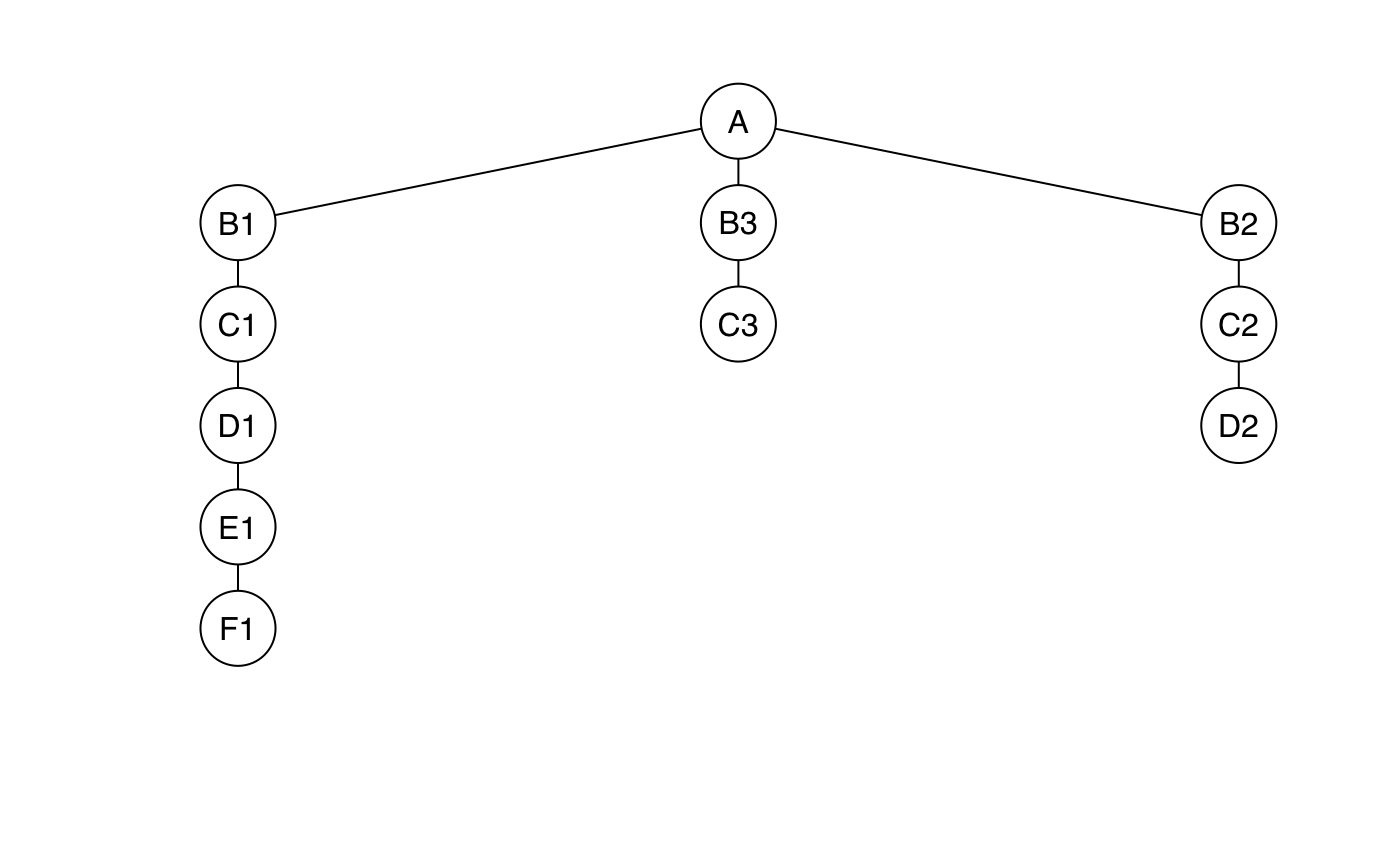
\includegraphics[width=10cm]{IMAGES/poset_3.png}
	\end{minipage}\hfill
	\begin{minipage}{0.4\linewidth}
		\label{table:student}
		\centering
        \begin{tabular}{l c c}
	& Elementi & Score & Ranking \\
	\hline
    \ang{1}	& A	& 0.60088088 \\		
    \ang{2}	& \color{blue}{B1} & 0.42157649 \\		
    \ang{3}	& \color{blue}{C1} & 0.40376571 \\	
    \ang{4}	& \color{blue}{D1} & 0.36724491 \\		
    \ang{5}	& \color{blue}{E1} & 0.30369488 \\		
    \ang{6}	& \color{blue}{F1} & 0.19696453 \\		
    \ang{7}	& \color{red}{B2} & 0.11167064 \\		
    \ang{8}	& \color{red}{C2} & 0.09696608 \\		
    \ang{9}	& \color{red}{D2} & 0.06569528 \\		
    \ang{10} & \color{green}{B3} & 0.06340602 \\
    \ang{11} & \color{green}{C3} & 0.04566517 \\	
    \hline
    \end{tabular}
    \caption{Ranking estratto dalla DS.\label{t:table}}
	\end{minipage}
\end{table}

Le catene sovra citate sono formate rispettivamente da 5, da 3 e da 2 elementi. Il ranking estratto dalla DS, come anticipato, assume una forma molto particolare in cui gli elementi sono ordinati a blocchi. La classifica è costituita da sotto ranking sistemati in ordine decrescente per numero di elementi dei sotto poset, questo risulta in un ranking molto lontano da quello che si estrarrebbe dalla MRP e, in generale, risulta anche illogico come tipo di classifica. La classifica che invece logicamente si vorrebbe riscontrare metterebbe gli elementi $B1$, $B2$ e $B3$ pari merito e così procedendo.


Sebbene quindi l'introduzione dell'elemento $Q$ come elemento massimo faccia si che la matrice DS non sia strutturata a blocchi, il tipo di ranking estratto risulta innaturale e messo a confronto con quello estratto dalla MRP risulta in valori di tau troppo bassi per ritenersi soddisfatti delle performance.


L'idea proposta per poter risolvere questo problema parte dall'aver osservato che per il poset in Figura 7.11, avendo quest'ultimo i sotto poset con lo stesso numero di elementi, il ranking viene fatto alla perfezione, ovvero quello estratto dalla matrice $Q$ coincide con quello estratto dalla matrice $M$.

\begin{figure}[H]
  \centering
  \begin{minipage}[b]{0.4\textwidth}
    \includegraphics[width=8cm]{IMAGES/poset_32.png}
  \end{minipage}
  \hfill
  \begin{minipage}[b]{0.4\textwidth}
    \includegraphics[width=8cm]{IMAGES/poset_32_05.png}
  \end{minipage}
  \caption{Poset inizialmente disgiunto con sotto poset di pari elementi unito e relative metriche di confronto ranking.}
\end{figure}

Questa osservazione risulta incredibilmente importante, poiché è stata fondamentale per ideare la soluzione al problema dei ranking di poset disgiunti.


Per poter comprendere pienamente il comportamento della matrice DS, si riportano nuovamente due poset (Figura 7.12). I sistemi parzialmente ordinati in questione sono entrambe frutto dell'unione di di un poset disgiunto costituito da due sotto poset attraverso l'elemento $Q$. L'unica differenza vigente per quanto riguarda questi due poset è l'elemento $x$, il quale fa si che nel poset a sinistra gli elementi dei due sotto poset siano in egual numero, mentre in quello di destra la proporzione di elementi sia sbilanciata di 1 appunto per questo elemento.

\begin{figure}[H]
  \centering
  \begin{minipage}[b]{0.4\textwidth}
    \includegraphics[width=8cm]{IMAGES/poset_33.png}
  \end{minipage}
  \hfill
  \begin{minipage}[b]{0.4\textwidth}
    \includegraphics[width=8cm]{IMAGES/poset_34.png}
  \end{minipage}
  \caption{Poset identici a parte per l'elemento $x$.}
\end{figure}

Si riporta ora il confronto dei ranking estratti usando i due diversi approcci. Per quanto riguarda il primo poset si ottiene un alto valore di tau, pari a 0.867. Osservando invece ora il poset a destra, la semplice aggiunta di un elemento, il quale fa si che i sotto poset abbiano numero di costituenti diverso, risulta nella logica espressa precedentemente, ovvero in una classifica fatta per ordine dei sotto poset (tutti gli elementi da $a$ ad $h$ sono classificati sotto gli elementi da $a2$ ad $x$) il che porta ad un valore di tau di appena 0.52.


Nel caso si immaginasse di prendere il poset a destra e di inserire un elemento $y$ dominato dall'elemento $h$ in modo da pareggiare nuovamente il numero di elementi tra sotto poset si tornerebbe ad un valore elevato di tau, pari a 0.894.


Questo tipo di comportamento, ovvero che il ranking della matrice $Q$ funziona efficacemente solo se i sotto poset hanno numero uguale di elementi, aiuta ad intuire la soluzione per poter applicare, nel modo più efficace possibile, l'estrazione del ranking dalla matrice DS per i poset disgiunti. Si è sperimentato che, per poter avere un ranking più simile possibile a quello estratto dalla matrice $M$, oltre ad aggiungere l'elemento $Q$ per rendere unito il poset disgiunto vadano aggiunti anche degli elementi (che verranno chiamati $x1, ...,xn$) al fine di pareggiare i sotto poset ed evitare il comportamento di classifica per ordine di numero di elementi che li compongono. Vine precisato che, come per l'elemento di unione $Q$, gli elementi $x1, ...,xn$ non devono essere riportati nel ranking finale.


Si riporta ora, in figura 7.13, il poset introdotto come esempio in Figura 7.10 al fine di poter estrarre il ranking nel modo più adatto dalla matrice $Q$. Come è stato introdotto precedentemente sono stati aggiunti tutti gli elementi artificiali per fare si che ciò sia possibile. Da principio si è aggiunto l'elemento $Q$ per unire il poset disgiunto ed evitare la composizione della matrice $Q$ a blocchi, poi sono stati aggiunti gli elementi da $x1$ ad $x5$ per pareggiare il sotto poset di soli due elementi con il sotto poset di sette elementi. Una volta attuate queste modifiche si procede con l'estrazione del ranking.

\begin{figure}[H]
  \centering
  \begin{minipage}[b]{0.4\textwidth}
    \includegraphics[width=8cm]{IMAGES/poset_27.png}
  \end{minipage}
  \hfill
  \begin{minipage}[b]{0.4\textwidth}
    \includegraphics[width=8cm]{IMAGES/poset_32_06.png}
  \end{minipage}
  \caption{Trasformazione del poset disgiunto per l'estrazione del ranking dalla DS.}
\end{figure}

In questo caso specifico, il confronto tra ranking passa da un valore di tau di 0.689 ad un valore di 0.833. La crescita di similarità dei ranking diventa ancora più accentuata su poset più complessi come si è osservato per quelli riportati in Figura 7.12.


In generale si può affermare che, con le dovute accortezze, la matrice DS continua a performare bene come alternativa alla MRP. Ovviamente, soprattutto per quanto riguarda questa tipologia di poset esposta nel paragrafo, si è notato come le due matrici differiscano in costruzione ed in comportamento, tuttavia attuando le giuste procedure è possibile ridurre queste differenze al minimo ed avere dei risultati accettabili.
\\~\\
Per riassumere i risultati osservati fino a questo momento, si può affermare che la matrice DS sembri, almeno per quanto riguarda i poset analizzati, essere considerabile come alternativa alla MRP. In generale si è osservato che raramente i ranking estratti coincidono alla perfezione ma tuttavia lo scheletro di fondo e il senso generale dell'ordinamento rimane lo stesso. Le piccole differenze riscontrate non cambiano l'interpretazione generale del ranking e molto spesso capita che consistano in semplici inversioni di elementi tra i due ranking.


Nonostante ci si sia interrogati sull'eventuale correlazione tra il valore di tau e il valore del rapporto di $C/I$, oppure con il numero di elementi del poset, o ancora solamente con il numero di comparabilità o incomparabilità, tuttavia non si sono riscontrate particolari tendenze degne di nota.


Chiaramente, quando è possibile applicarla, la MRP rimane la soluzione migliore, tuttavia in poset dalla complessità maggiore che, portano a far si che i tempi di computazione per quest'ultima non siano affrontabili, usare la matrice down-sets può essere considerata una soluzione valida purché si tenga a mente che essa non è infallibile. I ranking risultanti se interpretati come senso generale o struttura di fondo risultano molto potenti, tuttavia se si dovesse andare a ricercare delle informazioni più capillari questi ranking rischierebbero di essere imprecisi.


In conclusione i risultati ottenuti per questa matrice sono più che buoni ma, come detto in precedenza, l'utilizzo sostitutivo della MRP necessita consapevolezza dello strumento e l'interpretazione dei risultati necessita di essere filtrata con coscienza di causa. 


\chapter{Valutazione matrici alternative e complementari alla matrice DS}
Dopo aver osservato, nei capitoli precedenti, le caratteristiche, le performance e i comportamenti della matrice down-sets, si è giunti alla conclusione che essa risulti valida ma comunque (come ci si attendeva) non perfetta. Quello che ci si domanda ora è se utilizzando una logica di costruzione analoga si possano costruire matrici diverse, contenenti informazioni complementari, le quali siano in grado di emulare più efficientemente la matrice MRP e che quindi siano in grado di portare a ranking più simili ed avere un valore di tau maggiore.


Le strutture necessarie per poter definire queste matrici sono state esposte nel capitolo 6, in particolare si fa riferimento alla definizione di up-set (Definizione 6.0.4). La prima delle due matrici che si valuteranno come alternativa alla alla matrice DS è la matrice \textit{up-sets} (US). L'idea di base di questa nuova matrice è quella di comprendere l'informazione speculare rispetto alla matrice DS, ovvero l'informazione su come gli elementi facciano parte di up-set. Viene ora introdotta la matrice in questione.

\paragraph{Matrice up-sets}
La matrice US, come riportato poco sopra, parte dall'idea di cogliere quell'informazione speculare rispetto a quella della matrice DS. In seguito si valuteranno le performance di riproduzione dei ranking estratti con la MRP.


Indicando con $x_1, ..., x_n$ gli elementi dell'insieme $A$ sul quale viene definita la relazione d’ordine parziale $\unlhd$, la matrice up-sets, che verrà indicata come $Q^*$ (per evidenziare che nasce dall'idea della matrice $Q$), è una matrice $n\times n$ definita come segue:

\[Q^{*}_{ij} = \frac{|\{x_s\in A:x_j\unlhd x_s \land x_i\unlhd x_s\}|}{|\{x_s\in A:x_j\unlhd x_i\}|}.\]

Questo significa che $Q^{*}_{ij}$ è dato dal numero di elementi che l'up-set dell'elemento di colonna condivide con l'up-set dell'elemento di riga fratto il numero di elementi dell'up-set dell'elemento di colonna. In pratica il valore di $Q^{*}_{ij}$ esprime la percentuale dell'up-set di $x_j$ composta dall'up-set di $x_i$.


Come la matrice DS, se succede che $x_i\unlhd x_j$, ovvero se l'elemento di colonna domina l'elemento di riga, il valore di $Q^{*}_{ij}$ sarà 1 dato che l'up-set dell'elemento $x_j$ sarà chiaramente tutto contenuto nell'up-set di $x_i$. Da questo risulta che, ancora una volta come la matrice DS, la matrice US varrà 1 dove la matrice di dominanza $Z$ vale 1 ed il contrario. È possibile notare come osservando la matrice di dominanza per righe, si comprendono gli up-set generati dagli elementi di riga. Ne consegue che numeratore della formula per la matrice $Q^*$, ovvero il numero di elementi condivisi dai due up-set, è il numero di volte in cui due righe di $Z$ valgono entrambe 1 e il denominatore invece, ovvero il numero di elementi nell'up-set, è il numero di volte in cui la riga di $Z$ vale 1. Da questa osservazione si deduce la relazione tra le due matrici e ne deriva la formula per calcolare US partendo dalla matrice $Z$.

\[Q^{*}_{ij} = \frac{|Z_{j \cdot}=1 \land Z_{i \cdot}=1|}{|Z_{j \cdot}=1|}.\]

Come in precedenza per attuare l'operazione inversa e così ottenere la matrice di dominanza $Z$ a partire dalla matrice up-sets $Q^*$ basta porre a 0 tutte le entrate di quest'ultima che sono diverse da 1.


Per poter apprendere a pieno come la matrice US sia strutturata si riporta, come fatto per le altre matrici, la matrice estratta usando il poset in Figura 2.5.

$Q^*=$
\begin{blockarray}{ccccccccc}
& a & b & c & d & e  \\
\begin{block}{c(ccccccccc)}
  a & 1 & 0 & 1/2 & 1/3 & 1/5 \\
  b & 0 & 1 & 0 & 1/3 & 1/5 \\
  c & 1 & 0 & 1 & 1/3 & 2/5 \\
  d & 1 & 1 & 1/2 & 1 & 3/5 \\
  e & 1 & 1 & 1 & 1 & 1 \\
\end{block}
\end{blockarray}

Si osserva come la matrice US contenga l'informazione relativa agli up-set del poset di input. 


Per quanto riguardo ora la procedura di score, essa è analoga a quella vista per la matrice DS che poi di fatto proviene dalla procedura usata per la MRP.


La seconda matrice che viene introdotta come eventuale alternativa alla matrice MRP è una matrice che punta ad usare l'informazione sia dalla matrice DS che dalla matrice US. Questa matrice viene chiamata matrice \textit{sets-media} e viene ora introdotta.

\paragraph{Matrice sets-media}
Indicando con $x_1, ..., x_n$ gli elementi dell'insieme $A$ sul quale viene definita la relazione d’ordine parziale $\unlhd$, la matrice di sets-media, indicata come $Q^{\mu}$, è una matrice $n\times n$ definita come:

\[Q^{\mu}_{ij} =\frac{1}{2} (Q_{ij}+Q^{*}_{ij}) = \frac{1}{2} \left[ \left( \frac{|\{x_s\in A:x_s\unlhd x_i \land x_s\unlhd x_j\}|}{|\{x_s\in A:x_s\unlhd x_i\}|}\right) + \left( \frac{|\{x_s\in A:x_j\unlhd x_s \land x_i\unlhd x_s\}|}{|\{x_s\in A:x_j\unlhd x_i\}|}\right) \right].\]

In pratica le entrate della matrice $Q^{\mu}$ sono la media tra le entrate della matrice down-sets e della matrice up-sets. Questo fa si che la lettura della matrice non dia di per se un informazione direttamente riscontrabile sul poset ma fornisce invece un informazione media sulla potenza o importanza degli elementi. 


Per completezza, come per tutte le altre, si mostra ora la matrice $Q^{\mu}$ per il poset riportato in Figura 2.5.

$Q^{\mu}=$
\begin{blockarray}{ccccccccc}
& a & b & c & d & e  \\
\begin{block}{c(ccccccccc)}
  a & 1 & 0.25 & 0.5 & 0.417 & 0.225 \\
  b & 0.333 & 1 & 0.167 & 0.5 & 0.267 \\
  c & 1 & 0.25 & 1 & 0.417 & 0.45 \\
  d & 1 & 1 & 0.5 & 1 & 0.55 \\
  e & 1 & 1 & 1 & 1 & 1 \\
\end{block}
\end{blockarray}

Come si può chiaramente vedere, la matrice appena riportata è ottenuta tramite la media delle entrate della matrice DS e US ottenute a partire dal medesimo poset.


Per quanto riguarda la procedura di score, essa viene eseguita come per tutte le altre matrici viste fino a questo momento.
\\~\\
Una volta introdotte le due matrici, che verranno valutate per la forza dei ranking estratti da esse di riprodurre i ranking ottenuti dalla matrice MRP ed in base ai risultati ottenuti, verrà poi deciso in base alle performance se costituiscono una migliore alternativa rispetto alla DS.


In principio si sono testate le due nuove matrici, su tutti i poset del capitolo 7 usati per valutare le performance della matrice DS. È doveroso precisare che la matrice US necessita degli stessi accorgimenti introdotti per la matrice DS. Osservando i risultati su questi poset si è visto come la matrice US riscontri in tutti i casi dei risultati migliori rispetto alla matrice DS e come (da risultato attesto) la matrice sets-media si posizioni come una via di mezzo.


Si è scelto, al fine di non risultare ridondanti, di non riportare tutti i poset analizzati ma di sceglierne invece un paio di esempi esplicativi del risultato sopra riportato.
Il primo dei due poset riportato in Figura 26, è un poset disconnesso successivamente unito, con i rami di stessa dimensione.

\begin{figure}[H]
    \centering
    \includegraphics[width=8cm]{IMAGES/poset_33.png}
    \caption{Poset disgiunto formato da due poset incomparabili.}
    \label{fig:roc}
\end{figure}

Ora si riportano le metriche di valutazione per poter comprendere il risultato sopra riportato.
\begin{figure}[H]
  \centering
  \begin{minipage}[b]{0.4\textwidth}
    \includegraphics[width=8cm]{IMAGES/poset_33_1.png}
  \end{minipage}
  \hfill
  \begin{minipage}[b]{0.4\textwidth}
    \includegraphics[width=8cm]{IMAGES/poset_33_2.png}
  \end{minipage}
  \hfill
  \begin{minipage}[b]{0.4\textwidth}
    \includegraphics[width=8cm]{IMAGES/poset_33_3.png}
  \end{minipage}
  \caption{Valutazione dei ranking delle diverse matrici in confronto con quello della MRP.}
\end{figure}

Anche se non di molto si nota un aumento del tau per il ranking della matrice US, oltre a questo leggero innalzamento è visibile come il diagramma di Hasse sia molto più ordinato. In questo caso la matrice $Q^{\mu}$ non risulta in nessun miglioramento dalla matrice DS.


Si vuole ora riportare un secondo esempio del medesimo comportamento dove in Figura 28 è presente il poset già introdotto in precedenza tra i poset con poche comparabilità.

\begin{figure}[H]
    \centering
    \includegraphics[width=8cm]{IMAGES/poset_35.png}
    \caption{Poset con un rapporto $C/I$ poco elevato.}
    \label{fig:roc}
\end{figure}

Come in precedenza seguono le tre visualizzazioni grafiche (Figura 29) del confronto tra i ranking ottenuti dalle matrici e quello estratto dalla MRP, con relativo valore del coefficiente tau.

\begin{figure}[H]
  \centering
  \begin{minipage}[b]{0.4\textwidth}
    \includegraphics[width=8cm]{IMAGES/poset_35_1.png}
  \end{minipage}
  \hfill
  \begin{minipage}[b]{0.4\textwidth}
    \includegraphics[width=8cm]{IMAGES/poset_35_2.png}
  \end{minipage}
  \hfill
  \begin{minipage}[b]{0.4\textwidth}
    \includegraphics[width=8cm]{IMAGES/poset_35_3.png}
  \end{minipage}
  \caption{Valutazione dei ranking delle diverse matrici in confronto con quello della MRP.}
\end{figure}

Anche in questo caso si nota come il ranking prodotto dalla matrice US sia effettivamente migliore rispetto agli altri due, passando da un valore di tau di 0.845 ad un valore di 0.914. 


Osservando solamente i poset analizzati nel capitolo 7, come detto in precedenza, la matrice US ha sempre performance migliori e in alcuni casi anche in modo significativo. Dato questo risultato ci si domanda se questo sia valido in generale o solamente per alcuni tipi di poset. Si è osservato come in poset tendenzialmente chiusi, ovvero con pochi elementi massimali o minimali, le performance siano migliori usando la matrice US, come dimostrato su tutti i poset del capitolo 7.


Per quanto riguarda poset con più massimali o minimali la situazione invece è diversa. Si è osservato che se il poset in questione tende ad essere aperto verso l'alto, come il poset in Figura 8.5 il ranking della matrice US ha un calo di performance.

\begin{figure}[H]
    \centering
    \includegraphics[width=8cm]{IMAGES/poset_36.png}
    \caption{Poset con più elementi massimali.}
    \label{fig:roc}
\end{figure}

Per chiarire il comportamento appena citato si osservano, come di consueto, le metriche di confronto.

\begin{figure}[H]
  \centering
  \begin{minipage}[b]{0.4\textwidth}
    \includegraphics[width=8cm]{IMAGES/poset_36_1.png}
  \end{minipage}
  \hfill
  \begin{minipage}[b]{0.4\textwidth}
    \includegraphics[width=8cm]{IMAGES/poset_36_2.png}
  \end{minipage}
  \hfill
  \begin{minipage}[b]{0.4\textwidth}
    \includegraphics[width=8cm]{IMAGES/poset_36_3.png}
  \end{minipage}
  \caption{Valutazione dei ranking delle diverse matrici in confronto con quello della MRP.}
\end{figure}

Si osserva come la matrice $Q^*$ produca un ranking poco affidabile piazzandosi con un valore di tau di appena 0.4. Come ci si aspetta la matrice sets-media risulta una via di mezzo, ed in questo caso la scelta, di miglior alternativa alla matrice MRP, dovrebbe ricadere sulla matrice DS.


Osservando ora il poset in Figura 8.7, che di fatto corrisponde al ribaltamento del poset precedente, in modo da avere più elementi minimali ed essere aperto verso il basso, si vuole carpire la migliore alternativa in questo caso.

\begin{figure}[H]
    \centering
    \includegraphics[width=8cm]{IMAGES/poset_37.png}
    \caption{Poset con più elementi minimali.}
    \label{fig:roc}
\end{figure}

Si riportano ora le metriche di confronto dei ranking, per osservare a pieno il comportamento inverso atteso. 

Viene comunque ricordato che i poset ora riportati fungono solamente da vetrina, le prove sono state sperimentate su svariati poset con caratteristiche simili, i quali non vengono riportati per analogia di comportamenti delle matrici.

\begin{figure}[H]
  \centering
  \begin{minipage}[b]{0.4\textwidth}
    \includegraphics[width=8cm]{IMAGES/poset_37_1.png}
  \end{minipage}
  \hfill
  \begin{minipage}[b]{0.4\textwidth}
    \includegraphics[width=8cm]{IMAGES/poset_37_2.png}
  \end{minipage}
  \hfill
  \begin{minipage}[b]{0.4\textwidth}
    \includegraphics[width=8cm]{IMAGES/poset_37_3.png}
  \end{minipage}
  \caption{Valutazione dei ranking delle diverse matrici in confronto con quello della MRP.}
\end{figure}

In questo caso, si era previsto, si osserva il comportamento opposto, ovvero come la matrice $Q^*$ sia preferibile rispetto alla $Q$, e come al solito come la matrice $Q^{\mu}$ rimanga una solida via di mezzo.


Per concludere il ragionamento ci si chiede ora quale matrice sia preferibile per quanto riguarda poset aperti da ambo i lati, ovvero con più elementi massimali e più elementi minimali. 


In generale si è notato come la matrice US cali drasticamente per i poset aperti verso l'alto, mentre per quanto riguarda i poset aperti verso il basso, sebbene sia preferibile la US, la matrice DS non ha generalmente delle cattive performance. 


Per quanto riguarda ora i poset aperti da ambo i lati, si riporta come esempio e si analizza il poset in Figura 8.9.

\begin{figure}[H]
    \centering
    \includegraphics[width=8cm]{IMAGES/poset_38.png}
    \caption{Poset aperto da ambo i lati.}
    \label{fig:roc}
\end{figure}

Il poset appena presentato è caratterizzato da quattro elementi massimali e cinque elementi minimali. Ci si chiede ora quale delle alternative sia preferibile in questi casi.

\begin{figure}[H]
  \centering
  \begin{minipage}[b]{0.4\textwidth}
    \includegraphics[width=8cm]{IMAGES/poset_38_1.png}
  \end{minipage}
  \hfill
  \begin{minipage}[b]{0.4\textwidth}
    \includegraphics[width=8cm]{IMAGES/poset_38_2.png}
  \end{minipage}
  \hfill
  \begin{minipage}[b]{0.4\textwidth}
    \includegraphics[width=8cm]{IMAGES/poset_38_3.png}
  \end{minipage}
  \caption{Valutazione dei ranking delle diverse matrici in confronto con quello della MRP.}
\end{figure}

Osservando le metriche risulta chiaro come la matrice sets-media riporti le performance migliori a livello di similarità di ranking, viene però precisato come la matrice $Q$ in questo caso non si discosti di molto. Come da risultati precedenti, la matrice US risulta inadatta con la presenza di svariati elementi massimali.
\\~\\
Per concludere questo capitolo, si fa riferimento ai risultati ottenuti come riassunto. Si è osservato che per quanto riguarda poset tendenzialmente chiusi la matrice US risulta la scelta migliore, cosi come nel caso di poset con più elementi minimali, ma un numero contenuto di massimali. Successivamente si è osservato come, per i poset con un numero di elementi massimali elevato ma chiusi verso il basso, la matrice DS sia la scelta migliore. Infine per quanto riguarda i poset aperti da ambo i lati la matrice $Q^{\mu}$ performi meglio delle altre ma, comunque, anche la matrice $Q$ sia valutabile come alternativa.


In generale, come specificato più volte, la matrice MRP risulta sempre la migliore scelta se i tempi computazionali lo permettono, però in alternativa, qualora questi non lo permettessero, osservando il poset si può scegliere di utilizzare una tra la matrice down-sets, la matrice up-sets o la matrice sets-media, così da ottenere dei ranking comunque affidabili. L'affidabilità dei ranking fa comunque riferimento a quanto detto in conclusione al capitolo 7.

\chapter{Applicazioni ad un dataset reale}

Dopo aver studiato e confrontato le soluzioni proposte come alternativa alla matrice MRP, si vuole ora sperimentarne l'applicabilità in una situazione di utilizzo reale. Questa sezione funge da coda del percorso fatto fino a questo momento, il quale ha portato a perfezionamenti ed accortezze delle soluzioni proposte al fine di renderle effettivamente applicabili. Nonostante i dati che verranno utilizzati di seguito siano appunto reali e quindi i risultati ottenuti abbiano un senso e vadano interpretati, il fine dei calcoli che seguono non è l'analisi del problema in se, quanto piuttosto il mostrare come poter ottenere i risultati. Questa sezione ha la funzione di uno show-case dello strumento sviluppato nei capitoli precedenti.


Quello che verrà da prima fatto in questo paragrafo è la selezione di un dataset e la costruzione del relativo poset degli elementi che lo compongono. Una volta ottenuto il  poset se ne valuterà la forma e le caratteristiche per poter decidere quale tra le tre matrici \textit{down-sets}, \textit{up-sets} e \textit{sets-media} sia la migliore da utilizzare per poter ottenere un ranking quanto più possibile robusto.


\paragraph{Dati}
Per poter mostrare l'utilizzo delle matrici alternative alla MRP si sono adoperati dei dati presi dal dataset \citet{web:lang:stats} riguardante il sistema sanitario nei vari paesi del mondo.
Il dataset originariamente conteneva 14 variabili e 210 osservazioni. Le osservazioni rappresentano i paesi nel mondo e le variabili escluse le prime tre, le quali servono come indice, rappresentano degli indicatori inerenti al sistema sanitario. In particolare le variabili che compongono il dataset sono:

\begin{enumerate}
    \item \textbf{Country\_Region}: nome del paese.
    \item \textbf{Province\_State}: nome della suddivisione politica.
    \item \textbf{WorldBankName}: nome del paese usato da World Bank.
    \item \textbf{HealthexppctGDP2016}: livello di spesa sanitaria corrente espresso in percentuale del PIL. Le stime della spesa sanitaria corrente includono beni e servizi sanitari consumati durante ogni anno. Questo indicatore non include le spese sanitarie in conto capitale come edifici, macchinari, IT e scorte di vaccini per emergenze o focolai.
    \item \textbf{Healthexppublicpct2016}: quota della spesa sanitaria corrente finanziata da fonti pubbliche nazionali per la salute. Le fonti pubbliche nazionali includono entrate nazionali come trasferimenti interni e sovvenzioni, trasferimenti, sussidi a beneficiari di assicurazioni sanitarie volontarie, istituzioni senza scopo di lucro al servizio delle famiglie o schemi di finanziamento delle imprese, nonché pagamenti anticipati obbligatori e contributi di assicurazione sanitaria sociale. Non includono le risorse esterne spese dai governi per la salute.
    \item \textbf{Healthexpoutofpocketpct2016}: quota dei pagamenti diretti sul totale delle spese sanitarie correnti. I pagamenti di tasca propria sono spese per la salute direttamente di tasca propria dalle famiglie.
    \item \textbf{HealthexppercapitaUSD\_2016}: spese correnti per la salute pro capite in dollari USA correnti. Le stime della spesa sanitaria corrente includono beni e servizi sanitari consumati durante ogni anno.
    \item \textbf{percapitaexpPPP2016}: spese correnti pro capite per la salute espresse in dollari internazionali a parità di potere d'acquisto (PPP).
    \item \textbf{Externalhealthexppct2016}: quota della spesa sanitaria corrente finanziata da fonti esterne. Le fonti esterne sono costituite da trasferimenti esteri diretti e trasferimenti esteri distribuiti dal governo che comprendono tutti gli afflussi finanziari nel sistema sanitario nazionale dall'esterno del paese. Le fonti esterne fluiscono attraverso lo schema del governo o sono incanalate attraverso organizzazioni non governative o altri schemi.
    \item \textbf{Physiciansper1000\_2009.18}: i medici, includono medici generici e specialisti.
    \item \textbf{Nursemidwifeper10002009.18}: le infermiere e le ostetriche, includono infermieri professionisti, ostetriche professionisti, infermieri ausiliari, ostetriche ausiliarie, infermieri iscritti, ostetriche iscritte e altro personale associato, come infermieri dentali e infermieri di assistenza primaria.
    \item \textbf{Specialistsurgicalper10002008.18}: la forza lavoro chirurgica specializzata, è il numero di operatori specializzati in chirurgia, anestesia e ostetricia che lavorano in ciascun paese per 100.000 abitanti.
    \item \textbf{Completenessofbirthreg2009.18}: la completezza della registrazione delle nascite, è la percentuale di bambini di età inferiore ai 5 anni le cui nascite sono state registrate al momento dell'indagine. Il numeratore di completezza della registrazione di nascita include i bambini il cui certificato di nascita è stato visto dall'intervistatore o la cui madre o tutore afferma che la nascita è stata registrata.
    \item \textbf{Completenessofdeathreg2008.18}: la completezza della registrazione dei decessi, è la percentuale stimata di decessi registrati con le informazioni sulla causa di morte nel sistema di registrazione anagrafica di un paese.
\end{enumerate}

Di queste 14 variabili le prime tre sono state sostituite con il codice ISO dei paesi (sigla di tre lettere identificativa per ogni paese) per semplicità di raffigurazione del poset che ne deriva. Per quanto riguarda invece le altre variabili, la variabile \textbf{Externalhealthexppct2016} non è stata considerata in analisi per un duplice motivo, perché contiene troppi valori mancanti e perché la sua interpretazione può essere vista in modo ambiguo rispetto alle altre covariante; le restanti variabili invece sono state trasformate per divenire categoriali, il procedimento adoperato è stato quello di dividere l'intervallo in tre per tutte le variabili (a parte che per \textbf{percapitaexpPPP2016} che è stato diviso in quattro) e creare delle categorie del tipo "basso", "medio", "alto", per indicare il livello.


\section{Analisi}
Una volta ottenuto il dataset da analizzare si sono eliminate quelle osservazioni contenenti valori mancanti per non sporcare l'analisi. Dopo aver attuato questa pulizia i record sono passati da 210 a 66, e su questi ultimi si procede con l'analisi. Va sottolineato che qualora l'analisi su questo dataset avesse avuto scopo reale e non solamente di show-case, sarebbe stato necessario adoperare soluzioni alternative alla semplice eliminazione dei record con con valori mancanti, come ad esempio una stima i questi valori tramite modelli.


Come primo passo si costruisce il poset a partire dal dataset considerando quindi dieci variabili ordinali, di cui nove con tre categorie e una con quattro. Il poset che ne risulta è rappresentato in Figura 9.1. Va precisato che alcuni profili sono del tutto identici, per questo motivo quei paesi non sono stati separati in elementi ma piuttosto uniti sotto lo stesso.

\begin{figure}[H]
    \centering
    \includegraphics[width=12cm]{IMAGES/poset_fin.png}
    \caption{Poset del sistema sanitario di 66 paesi nel mondo.}
    \label{fig:roc}
\end{figure}

Il poset ottenuto è evidentemente molto complesso, infatti esso è caratterizzato da 66 elementi con 595 comparabilità e 1550 incomparabilità. Risulta quindi chiaro come il calcolo della matrice MRP su questo sistema parzialmente ordinato sia di fatto impossibile da effettuare in tempi utili. In questo caso la soluzione da adoperare è l'utilizzo di una delle tre matrici proposte come alternativa alla muitual ranking probability. Dato che il poset in questione ha 10 elementi massimali e 5 elementi minimali è considerabile un poset aperto da entrambe i lati e per questo motivo la scelta per la matrice da utilizzare ricade sulla matrice $Q^{\mu}$.  Va ricordato che in questo caso anche la matrice $Q$ sarebbe una scelta possibile dato che, come si è osservato, ha delle performance paragonabili a quelle della matrice sets-media; la cosa importante è non utilizzare la matrice $Q^{*}$ dato che con i poset aperti verso l'alto performa male.


\section{Risultati}
Una volta scelta la matrice ideale, quindi in questo caso la matrice sets-media, la si calcola e si estrapola lo score, dal quale si ottiene il ranking che posiziona i 66 paesi in ordine di livello sanitario. Si ricorda che il ranking ottenuto non sarà perfettamente concordante da quello che si sarebbe ottenuto dalla matrice MRP, tuttavia il senso generale e lo scheletro sono, come si è visto in precedenza, affidabili. Si ricorda che per il ranking non è possibile fare affidamento su quanto visibile ad occhio nel poset poiché è troppo complesso e perché la forma così simmetrica è ottenuta volontariamente a discapito del posizionamento "naturale" degli elementi. Si riporta ora in Tabella 9.1 parte del ranking ottenuto dalla procedura applicata.

\begin{table}[H]
\centering
	\begin{tabular}{l c c}
	& ISO & Paese & Posizione\\
	\hline
	\ang{1} &  CHE & Svizzera \\
	\ang{2}  & MLT & Malta\\
	\ang{3} & PRT & Portogallo\\
	\ldots & \ldots & \ldots\\
	\ang{36} & ITA,CZE & Italia, Rep. Ceca\\
	\ldots & \ldots & \ldots\\
	\ang{65} & ALB & Albania\\
	\ang{66} & EGY & Egitto\\
	\ang{67} & IRQ & Iraq\\
	\hline
	\end{tabular}
\caption{Ranking dei paesi nel mondo per livello sanitario.\label{t:table}}
\end{table}

Il ranking ottenuto vede la Svizzera in prima posizione, seguita da Malta e dal Portogallo, mentre alla coda della classifica troviamo paesi quali Albania, Egitto e Iraq. Va precisato che oltre ad avere livelli bassi i paesi che si trovano sul fondo della classifica sono dotati anche di incomparabilità elevata, dato che come si è visto precedentemente, queste matrici tendono ad abbassare gli elementi più incomparabili. Nonostante non ci sia una controparte prodotta dalla MRP, il ranking anche a livello empirico di "esperienza" sembra sensato. Come ultima nota si riporta che l'Italia si posiziona (insieme alla Repubblica Ceca) a metà classifica in trentaseiesima posizione. 


Ricordando che l'analisi non è in nessun modo affidabile, per come sono state trasformate le variabili (i livelli sono stati scelti empiricamente e non usando informazioni riscontrabili), per la presenza di pochi paesi a causa di molti valori mancanti e per l'inesperienza sull'argomento e sulle variabili; tuttavia se si vuole dare un'interpretazione, che però lascia il tempo che trova, il livello sanitario di un paese sviluppato come l'Italia è quantomeno mediocre rispetto ad altri paesi presenti nell'unione europea. Per quanto riguarda le posizioni estreme (testa e coda della classifica) esse erano abbastanza attese.
\\~\\
Come ultima nota si riporta come lo strumento abbia lavorato in modo efficace per ottenere un ranking quantomeno sensato, ovviamente la debolezza dei ranking estratti con questo metodo risiede nella capillarità ma il senso generale risulta affidabile ed utilizzabile come alternativa valida alla matrice MRP.

\chapter{Conclusione}
Come conclusione del percorso fatto in questa tesi si vogliono riprendere passo dopo passo gli argomenti, i calcoli e i risultati ottenuti per poter fare un sunto e concludere con le dovute riflessioni.


Da principio si è prestata particolare importanza alle strutture dei poset, strutture che si sono dimostrate fondamentali per trattare i dati ordinali ma, tuttavia, per quanto perfette nella teoria, troppo complesse nella pratica del calcolo della loro forma matriciale per l'estrazione di ranking.  I risultati cercati ed ottenuti hanno sempre avuto lo scopo di poter trovare una soluzione al problema computazionale nel calcolo della matrice MRP dei poset. Più che una soluzione quella che in realtà si è trovata è un alternativa, dato che si è visto che la strada delle soluzioni non porta a risultati soddisfacenti. Dopo aver esposto il problema computazionale e i problemi relativi alle soluzioni canoniche, si è proposta la matrice \textit{down-sets}, la quale essendo più facile da calcolare della MRP ma, nonostante questo, contenendo informazioni aggiuntive rispetto alle matrici di copertura e dominanza, avrebbe potuto essere un'alternativa valida. Definita la matrice se ne sono studiate le proprietà e i comportamenti, e attraverso un confronto diretto con la matrice MRP si è visto come la matrice $Q$ ottenesse delle buone performance nel produrre i ranking. Durante questo processo sono state smussate e corretti i comportamenti della matrice su alcuni tipi di poset. Una volta studiata la matrice alternativa è risultato naturale interrogarsi su come altre due matrice, ovvero la matrice \textit{up-sets} e la matrice \textit{sets-media}, che nascono dalla stessa idea da cui nasce la matrice down-sets. Una volta studiate e confrontate le matrici su svariati tipi di poset si è potuto fare un ragionamento completo e dedurne una regola per l'utilizzo delle tre matrici a seconda delle situazioni. Infine come dimostrazione dello strumento sviluppato si è attuata un'analisi sui dei dati reali, sui quali sarebbe stato impossibile produrre un poset utilizzando la matrice MRP.


I risultati ottenuti durante il percorso suggeriscono come le tre matrici $Q$, $Q^{*}$ e $Q^{\mu}$ siano una valida alternativa alla matrice MRP per ottenere i ranking dai poset. Rimane necessario precisare quanto affermato a fine capitolo 7, ovvero che la forza di questi strumenti risiede nel riuscire a replicare il senso generale del ranking che sarebbe stato prodotto dalla MRP, ma risultano più deboli se si vuole osservare il ranking elemento per elemento nella sua capillarità. 


Per quanto riguarda l'utilizzo pratico di queste tre matrici, si ricorda che sono necessari gli accorgimenti introdotti nella sezione 7.5 per quanto riguarda i poset disgiunti. Per quanto riguarda invece la scelta tra le tre matrici $Q$, $Q^{*}$ e $Q^{\mu}$ è necessario osservare il numero di elementi massimali e minimali del poset, come precisato alla fine del capitolo 8, e qualora il poset sia chiuso da ambo i lati o solamente verso l'alto la scelta migliore sarebbe la matrice up-sets, per poset chiusi verso il basso ma aperti verso l'altro si dovrebbe utilizzare la matrice down-sets ed infine per i poset aperti da ambo i lati la scelta ricade sulla matrice sets-media.


Come conclusione si ricorda che, sebbene i risultati ottenuti siano positivi e le matrici di fatto rappresentino una valida alternativa alla matrice MRP, il lavoro da svolgere in ambito di ricerca per l'utilizzo efficace dei poset è ancora tanto e per questo motivo si sprona chiunque abbia interesse nell'argomento a sperimentare e ricercare soluzioni alternative o a perfezionare quelle già proposte, al fine di poter perfezionare l'utilizzo di queste strutture così necessarie in statistica e non solo per il trattamento dei dati ordinali.

\bibliographystyle{apalike.bst}
\bibliography{citations.bib}

%%%%
\chapter*{Ringraziamenti}
\addcontentsline{toc}{chapter}{Ringraziamenti}
\chaptermark{Ringraziamenti}
\rhead{}

Un doveroso e sincero grazie al mio Relatore, il Professore Marco Fattore, che mi ha permesso di lavorare e appassionarmi nella scrittura e ricerca per questo progetto di tesi e per aver rappresentato un punto di riferimento durante questi mesi.


Ringrazio profondamente tutti i Professori che ho avuto il piacere di incontrare e da cui ho avuto l'onore di apprendere durante questi tre anni, per aver reso possibile questo mio traguardo. In particolare ringrazio la Professoressa Paola Chiodini per avermi fatto comprendere la necessità dell'impegno ad affiancare la passione per poter ottenere grandi risultati e ringrazio profondamente il Professore Fabio Mercorio per aver trasformato la mia passione per la statistica in amore.


Grazie ai miei compagni di corso, in particolare a Kado e Fossa per aver resistito insieme a me, per aver condiviso la mia passione e per avermi concesso di condividere con loro questo mio percorso di crescita.


Colgo l'occasione per poter dire un grazie di cuore ai miei Genitori a cui devo tutto. Grazie per avermi sempre sostenuto e per avermi reso la persona che sono. Un grazie a mio papà Francesco per avermi insegnato a guardare lontano e un grazie a mia mamma Barbara per avermi insegnato la forza e la volontà d'animo.


Grazie a Sofia, la miglior sorella che potessi mai desiderare, per essere nella mia vita, per avermi sopportato durante tutti questi anni
e per avermi reso, cosa che sempre farà, orgoglioso dei suoi traguardi.


Grazie a tutta la mia famiglia per essersi presa cura di me, per avermi fatto crescere e per avermi fatto sentire di appartenere a qualcosa di speciale.


Grazie a Sara per avermi sostenuto sempre, per avermi spronato ogni giorno, per avermi consolato nelle mie sconfitte e per aver festeggiato con più gioia di tutti quanti per le mie vittorie. Ti ringrazio per esserci stata sempre, ogni secondo; ti ringrazio davvero, tutto questo è anche merito tuo.


Un grazie a tutti gli amici che sono che sono cresciuti con me e che hanno sempre riempito di vita la mia vita, un grazie a Maio, Kappa, Bobbi, Marta, Ali, Chiara, Edo, Berto, Dani, Lollo, Kiki, Cri, Michi, Ele, Cesca e Simo.


Un grazie anche a tutti voi che state leggendo questi ringraziamenti, se siete qui a leggere le mie parole vuol dire che avete contribuito a questo mio grande traguardo e di questo vi ringrazio con tutto il cuore.



\end{document}


